% Options for packages loaded elsewhere
\PassOptionsToPackage{unicode}{hyperref}
\PassOptionsToPackage{hyphens}{url}
\documentclass[
]{article}
\usepackage{xcolor}
\usepackage[margin=1in]{geometry}
\usepackage{amsmath,amssymb}
\setcounter{secnumdepth}{-\maxdimen} % remove section numbering
\usepackage{iftex}
\ifPDFTeX
  \usepackage[T1]{fontenc}
  \usepackage[utf8]{inputenc}
  \usepackage{textcomp} % provide euro and other symbols
\else % if luatex or xetex
  \usepackage{unicode-math} % this also loads fontspec
  \defaultfontfeatures{Scale=MatchLowercase}
  \defaultfontfeatures[\rmfamily]{Ligatures=TeX,Scale=1}
\fi
\usepackage{lmodern}
\ifPDFTeX\else
  % xetex/luatex font selection
\fi
% Use upquote if available, for straight quotes in verbatim environments
\IfFileExists{upquote.sty}{\usepackage{upquote}}{}
\IfFileExists{microtype.sty}{% use microtype if available
  \usepackage[]{microtype}
  \UseMicrotypeSet[protrusion]{basicmath} % disable protrusion for tt fonts
}{}
\makeatletter
\@ifundefined{KOMAClassName}{% if non-KOMA class
  \IfFileExists{parskip.sty}{%
    \usepackage{parskip}
  }{% else
    \setlength{\parindent}{0pt}
    \setlength{\parskip}{6pt plus 2pt minus 1pt}}
}{% if KOMA class
  \KOMAoptions{parskip=half}}
\makeatother
\usepackage{color}
\usepackage{fancyvrb}
\newcommand{\VerbBar}{|}
\newcommand{\VERB}{\Verb[commandchars=\\\{\}]}
\DefineVerbatimEnvironment{Highlighting}{Verbatim}{commandchars=\\\{\}}
% Add ',fontsize=\small' for more characters per line
\usepackage{framed}
\definecolor{shadecolor}{RGB}{248,248,248}
\newenvironment{Shaded}{\begin{snugshade}}{\end{snugshade}}
\newcommand{\AlertTok}[1]{\textcolor[rgb]{0.94,0.16,0.16}{#1}}
\newcommand{\AnnotationTok}[1]{\textcolor[rgb]{0.56,0.35,0.01}{\textbf{\textit{#1}}}}
\newcommand{\AttributeTok}[1]{\textcolor[rgb]{0.13,0.29,0.53}{#1}}
\newcommand{\BaseNTok}[1]{\textcolor[rgb]{0.00,0.00,0.81}{#1}}
\newcommand{\BuiltInTok}[1]{#1}
\newcommand{\CharTok}[1]{\textcolor[rgb]{0.31,0.60,0.02}{#1}}
\newcommand{\CommentTok}[1]{\textcolor[rgb]{0.56,0.35,0.01}{\textit{#1}}}
\newcommand{\CommentVarTok}[1]{\textcolor[rgb]{0.56,0.35,0.01}{\textbf{\textit{#1}}}}
\newcommand{\ConstantTok}[1]{\textcolor[rgb]{0.56,0.35,0.01}{#1}}
\newcommand{\ControlFlowTok}[1]{\textcolor[rgb]{0.13,0.29,0.53}{\textbf{#1}}}
\newcommand{\DataTypeTok}[1]{\textcolor[rgb]{0.13,0.29,0.53}{#1}}
\newcommand{\DecValTok}[1]{\textcolor[rgb]{0.00,0.00,0.81}{#1}}
\newcommand{\DocumentationTok}[1]{\textcolor[rgb]{0.56,0.35,0.01}{\textbf{\textit{#1}}}}
\newcommand{\ErrorTok}[1]{\textcolor[rgb]{0.64,0.00,0.00}{\textbf{#1}}}
\newcommand{\ExtensionTok}[1]{#1}
\newcommand{\FloatTok}[1]{\textcolor[rgb]{0.00,0.00,0.81}{#1}}
\newcommand{\FunctionTok}[1]{\textcolor[rgb]{0.13,0.29,0.53}{\textbf{#1}}}
\newcommand{\ImportTok}[1]{#1}
\newcommand{\InformationTok}[1]{\textcolor[rgb]{0.56,0.35,0.01}{\textbf{\textit{#1}}}}
\newcommand{\KeywordTok}[1]{\textcolor[rgb]{0.13,0.29,0.53}{\textbf{#1}}}
\newcommand{\NormalTok}[1]{#1}
\newcommand{\OperatorTok}[1]{\textcolor[rgb]{0.81,0.36,0.00}{\textbf{#1}}}
\newcommand{\OtherTok}[1]{\textcolor[rgb]{0.56,0.35,0.01}{#1}}
\newcommand{\PreprocessorTok}[1]{\textcolor[rgb]{0.56,0.35,0.01}{\textit{#1}}}
\newcommand{\RegionMarkerTok}[1]{#1}
\newcommand{\SpecialCharTok}[1]{\textcolor[rgb]{0.81,0.36,0.00}{\textbf{#1}}}
\newcommand{\SpecialStringTok}[1]{\textcolor[rgb]{0.31,0.60,0.02}{#1}}
\newcommand{\StringTok}[1]{\textcolor[rgb]{0.31,0.60,0.02}{#1}}
\newcommand{\VariableTok}[1]{\textcolor[rgb]{0.00,0.00,0.00}{#1}}
\newcommand{\VerbatimStringTok}[1]{\textcolor[rgb]{0.31,0.60,0.02}{#1}}
\newcommand{\WarningTok}[1]{\textcolor[rgb]{0.56,0.35,0.01}{\textbf{\textit{#1}}}}
\usepackage{longtable,booktabs,array}
\newcounter{none} % for unnumbered tables
\usepackage{calc} % for calculating minipage widths
% Correct order of tables after \paragraph or \subparagraph
\usepackage{etoolbox}
\makeatletter
\patchcmd\longtable{\par}{\if@noskipsec\mbox{}\fi\par}{}{}
\makeatother
% Allow footnotes in longtable head/foot
\IfFileExists{footnotehyper.sty}{\usepackage{footnotehyper}}{\usepackage{footnote}}
\makesavenoteenv{longtable}
\usepackage{graphicx}
\makeatletter
\newsavebox\pandoc@box
\newcommand*\pandocbounded[1]{% scales image to fit in text height/width
  \sbox\pandoc@box{#1}%
  \Gscale@div\@tempa{\textheight}{\dimexpr\ht\pandoc@box+\dp\pandoc@box\relax}%
  \Gscale@div\@tempb{\linewidth}{\wd\pandoc@box}%
  \ifdim\@tempb\p@<\@tempa\p@\let\@tempa\@tempb\fi% select the smaller of both
  \ifdim\@tempa\p@<\p@\scalebox{\@tempa}{\usebox\pandoc@box}%
  \else\usebox{\pandoc@box}%
  \fi%
}
% Set default figure placement to htbp
\def\fps@figure{htbp}
\makeatother
\setlength{\emergencystretch}{3em} % prevent overfull lines
\providecommand{\tightlist}{%
  \setlength{\itemsep}{0pt}\setlength{\parskip}{0pt}}
\usepackage{bookmark}
\IfFileExists{xurl.sty}{\usepackage{xurl}}{} % add URL line breaks if available
\urlstyle{same}
% fallback for those not using the hyperref driver hyperxmp:
\makeatletter
\@ifundefined{xmpquote}{\newcommand{\xmpquote}[1]{#1}}{}
\makeatother
\hypersetup{
  pdftitle={Final Assessment --- Introduction to Data Science},
  pdfauthor={Ruhan Shafi (u3284342), University of Canberra},
  hidelinks,
  pdfcreator={LaTeX via pandoc}}

\title{Final Assessment --- Introduction to Data Science}
\usepackage{etoolbox}
\makeatletter
\providecommand{\subtitle}[1]{% add subtitle to \maketitle
  \apptocmd{\@title}{\par {\large #1 \par}}{}{}
}
\makeatother
\subtitle{11372 \& 11516}
\author{Ruhan Shafi (u3284342), University of Canberra}
\date{10 November 2026}

\begin{document}
\maketitle

{
\setcounter{tocdepth}{2}
\tableofcontents
}
\begin{Shaded}
\begin{Highlighting}[]
\NormalTok{knitr}\SpecialCharTok{::}\NormalTok{opts\_chunk}\SpecialCharTok{$}\FunctionTok{set}\NormalTok{(}\AttributeTok{echo =} \ConstantTok{TRUE}\NormalTok{, }\AttributeTok{warning =} \ConstantTok{FALSE}\NormalTok{, }\AttributeTok{message =} \ConstantTok{FALSE}\NormalTok{)}

\DocumentationTok{\#\# {-}{-}{-}{-}{-}{-}{-}{-}{-}{-}{-}{-}{-}{-}{-}{-}{-}{-}{-}{-}{-}{-}{-}{-}{-}{-}{-}{-}{-}{-}{-}{-}{-}{-}{-}{-}{-}{-}{-}{-}{-}{-}{-}{-}{-}{-}{-}{-}{-}{-}{-}{-}{-}{-}{-}{-}{-}{-}{-}{-}{-}{-}{-}{-}{-}{-}{-}{-}{-}{-}{-}{-}{-}{-}}
\DocumentationTok{\#\#  DO NOT EDIT personalise.R. Run this chunk once to build your dataset.}
\DocumentationTok{\#\# {-}{-}{-}{-}{-}{-}{-}{-}{-}{-}{-}{-}{-}{-}{-}{-}{-}{-}{-}{-}{-}{-}{-}{-}{-}{-}{-}{-}{-}{-}{-}{-}{-}{-}{-}{-}{-}{-}{-}{-}{-}{-}{-}{-}{-}{-}{-}{-}{-}{-}{-}{-}{-}{-}{-}{-}{-}{-}{-}{-}{-}{-}{-}{-}{-}{-}{-}{-}{-}{-}{-}{-}{-}{-}}
\FunctionTok{source}\NormalTok{(}\StringTok{"personalise.R"}\NormalTok{)}

\NormalTok{my }\OtherTok{\textless{}{-}} \FunctionTok{make\_my\_dataset}\NormalTok{(params}\SpecialCharTok{$}\NormalTok{studentID,}
                      \AttributeTok{raw\_dir =} \StringTok{"data\_raw"}\NormalTok{,}
                      \AttributeTok{out\_dir =} \StringTok{"data"}\NormalTok{)}
\end{Highlighting}
\end{Shaded}

\begin{verbatim}
## Student ID   : u3284342 
## Seed         : 12109058 
## Window       : 2004 - 2023 
## Countries    : 150 
## Files written to /home/ruhanshafi/Projects/IntroDS/Assessment2/data 
##   Emissions.csv   3005 rows
##   Renewables.csv  148 rows x 21 cols
##   Consumption.csv 1897 rows
##   Countries.csv   150 rows
## FINGERPRINT  : EM-606669-0798-6584
\end{verbatim}

\begin{Shaded}
\begin{Highlighting}[]
\CommentTok{\# Packages used in this report. Install once with:}
\CommentTok{\# install.packages(c("tidyverse", "lubridate", "scales", "knitr",}
\CommentTok{\#                    "glmnet", "rpart"))}
\FunctionTok{library}\NormalTok{(tidyverse)  }\CommentTok{\# dplyr, tidyr, readr, stringr, forcats, ggplot2}
\FunctionTok{library}\NormalTok{(lubridate)  }\CommentTok{\# robust parsing of the inconsistent Year formats}
\FunctionTok{library}\NormalTok{(scales)     }\CommentTok{\# comma and log{-}scale axis labels}
\FunctionTok{library}\NormalTok{(knitr)      }\CommentTok{\# kable() tables}
\FunctionTok{library}\NormalTok{(glmnet)     }\CommentTok{\# ridge and lasso regression (Task 3.8)}
\FunctionTok{library}\NormalTok{(rpart)      }\CommentTok{\# regression tree (Task 3.8)}

\FunctionTok{theme\_set}\NormalTok{(}\FunctionTok{theme\_minimal}\NormalTok{(}\AttributeTok{base\_size =} \DecValTok{11}\NormalTok{))}
\end{Highlighting}
\end{Shaded}

\begin{Shaded}
\begin{Highlighting}[]
\CommentTok{\# Helper functions used throughout Task 1. Function names follow Google\textquotesingle{}s}
\CommentTok{\# R Style Guide (BigCamelCase); objects use snake\_case.}

\CommentTok{\# Convert text to numbers, tolerating thousands separators, currency}
\CommentTok{\# symbols, stray spaces and the Unicode minus sign. Anything that still is}
\CommentTok{\# not a number becomes NA, so it can be counted as a defect.}
\NormalTok{ToNumber }\OtherTok{\textless{}{-}} \ControlFlowTok{function}\NormalTok{(x) \{}
\NormalTok{  x }\OtherTok{\textless{}{-}} \FunctionTok{str\_replace\_all}\NormalTok{(}\FunctionTok{as.character}\NormalTok{(x), }\StringTok{"−"}\NormalTok{, }\StringTok{"{-}"}\NormalTok{)}
\NormalTok{  x }\OtherTok{\textless{}{-}} \FunctionTok{str\_remove\_all}\NormalTok{(x, }\StringTok{"[,$}\SpecialCharTok{\textbackslash{}\textbackslash{}}\StringTok{s]"}\NormalTok{)}
  \FunctionTok{suppressWarnings}\NormalTok{(}\FunctionTok{as.numeric}\NormalTok{(x))}
\NormalTok{\}}

\CommentTok{\# Label each Year value by its format, so the variants can be reported.}
\NormalTok{ClassifyYearFormat }\OtherTok{\textless{}{-}} \ControlFlowTok{function}\NormalTok{(x) \{}
\NormalTok{  x }\OtherTok{\textless{}{-}} \FunctionTok{str\_trim}\NormalTok{(}\FunctionTok{as.character}\NormalTok{(x))}
  \FunctionTok{case\_when}\NormalTok{(}
    \FunctionTok{is.na}\NormalTok{(x) }\SpecialCharTok{|}\NormalTok{ x }\SpecialCharTok{==} \StringTok{""} \SpecialCharTok{\textasciitilde{}} \StringTok{"missing"}\NormalTok{,}
    \FunctionTok{str\_detect}\NormalTok{(x, }\StringTok{"\^{}}\SpecialCharTok{\textbackslash{}\textbackslash{}}\StringTok{d\{4\}$"}\NormalTok{) }\SpecialCharTok{\textasciitilde{}} \StringTok{"YYYY"}\NormalTok{,}
    \FunctionTok{str\_detect}\NormalTok{(x, }\StringTok{"\^{}}\SpecialCharTok{\textbackslash{}\textbackslash{}}\StringTok{d\{4\}}\SpecialCharTok{\textbackslash{}\textbackslash{}}\StringTok{.0+$"}\NormalTok{) }\SpecialCharTok{\textasciitilde{}} \StringTok{"YYYY.0 (decimal)"}\NormalTok{,}
    \FunctionTok{str\_detect}\NormalTok{(x, }\StringTok{"\^{}}\SpecialCharTok{\textbackslash{}\textbackslash{}}\StringTok{d\{4\}{-}}\SpecialCharTok{\textbackslash{}\textbackslash{}}\StringTok{d\{1,2\}{-}}\SpecialCharTok{\textbackslash{}\textbackslash{}}\StringTok{d\{1,2\}"}\NormalTok{) }\SpecialCharTok{\textasciitilde{}} \StringTok{"ISO date (YYYY{-}MM{-}DD)"}\NormalTok{,}
    \FunctionTok{str\_detect}\NormalTok{(x, }\StringTok{"\^{}}\SpecialCharTok{\textbackslash{}\textbackslash{}}\StringTok{d\{1,2\}[/.{-}]}\SpecialCharTok{\textbackslash{}\textbackslash{}}\StringTok{d\{1,2\}[/.{-}]}\SpecialCharTok{\textbackslash{}\textbackslash{}}\StringTok{d\{4\}$"}\NormalTok{) }\SpecialCharTok{\textasciitilde{}} \StringTok{"D/M/YYYY date"}\NormalTok{,}
    \FunctionTok{str\_detect}\NormalTok{(x, }\StringTok{"\^{}}\SpecialCharTok{\textbackslash{}\textbackslash{}}\StringTok{d\{5\}$"}\NormalTok{) }\SpecialCharTok{\textasciitilde{}} \StringTok{"Excel serial number"}\NormalTok{,}
    \FunctionTok{str\_detect}\NormalTok{(x, }\StringTok{"\^{}\textquotesingle{}?}\SpecialCharTok{\textbackslash{}\textbackslash{}}\StringTok{d\{2\}$"}\NormalTok{) }\SpecialCharTok{\textasciitilde{}} \StringTok{"two{-}digit year"}\NormalTok{,}
    \FunctionTok{str\_detect}\NormalTok{(x, }\StringTok{"[A{-}Za{-}z]"}\NormalTok{) }\SpecialCharTok{\&} \FunctionTok{str\_detect}\NormalTok{(x, }\StringTok{"}\SpecialCharTok{\textbackslash{}\textbackslash{}}\StringTok{d\{4\}"}\NormalTok{) }\SpecialCharTok{\textasciitilde{}} \StringTok{"text + year"}\NormalTok{,}
    \ConstantTok{TRUE} \SpecialCharTok{\textasciitilde{}} \StringTok{"other"}
\NormalTok{  )}
\NormalTok{\}}

\CommentTok{\# Convert every Year variant to a four{-}digit integer year.}
\NormalTok{ParseYear }\OtherTok{\textless{}{-}} \ControlFlowTok{function}\NormalTok{(x) \{}
\NormalTok{  x }\OtherTok{\textless{}{-}} \FunctionTok{str\_trim}\NormalTok{(}\FunctionTok{as.character}\NormalTok{(x))}
\NormalTok{  fmt }\OtherTok{\textless{}{-}} \FunctionTok{ClassifyYearFormat}\NormalTok{(x)}
\NormalTok{  out }\OtherTok{\textless{}{-}} \FunctionTok{rep}\NormalTok{(}\ConstantTok{NA\_integer\_}\NormalTok{, }\FunctionTok{length}\NormalTok{(x))}

\NormalTok{  idx }\OtherTok{\textless{}{-}}\NormalTok{ fmt }\SpecialCharTok{\%in\%} \FunctionTok{c}\NormalTok{(}\StringTok{"YYYY"}\NormalTok{, }\StringTok{"YYYY.0 (decimal)"}\NormalTok{, }\StringTok{"ISO date (YYYY{-}MM{-}DD)"}\NormalTok{)}
\NormalTok{  out[idx] }\OtherTok{\textless{}{-}} \FunctionTok{as.integer}\NormalTok{(}\FunctionTok{str\_sub}\NormalTok{(x[idx], }\DecValTok{1}\NormalTok{, }\DecValTok{4}\NormalTok{))}

\NormalTok{  idx }\OtherTok{\textless{}{-}}\NormalTok{ fmt }\SpecialCharTok{==} \StringTok{"D/M/YYYY date"}
\NormalTok{  out[idx] }\OtherTok{\textless{}{-}} \FunctionTok{year}\NormalTok{(}\FunctionTok{parse\_date\_time}\NormalTok{(x[idx], }\AttributeTok{orders =} \FunctionTok{c}\NormalTok{(}\StringTok{"dmy"}\NormalTok{, }\StringTok{"mdy"}\NormalTok{)))}

\NormalTok{  idx }\OtherTok{\textless{}{-}}\NormalTok{ fmt }\SpecialCharTok{==} \StringTok{"Excel serial number"}
\NormalTok{  out[idx] }\OtherTok{\textless{}{-}} \FunctionTok{year}\NormalTok{(}\FunctionTok{as\_date}\NormalTok{(}\FunctionTok{as.numeric}\NormalTok{(x[idx]), }\AttributeTok{origin =} \StringTok{"1899{-}12{-}30"}\NormalTok{))}

\NormalTok{  idx }\OtherTok{\textless{}{-}}\NormalTok{ fmt }\SpecialCharTok{==} \StringTok{"two{-}digit year"}
\NormalTok{  yy }\OtherTok{\textless{}{-}} \FunctionTok{as.integer}\NormalTok{(}\FunctionTok{str\_remove}\NormalTok{(x[idx], }\StringTok{"\textquotesingle{}"}\NormalTok{))}
\NormalTok{  out[idx] }\OtherTok{\textless{}{-}} \FunctionTok{if\_else}\NormalTok{(yy }\SpecialCharTok{\textgreater{}} \DecValTok{50}\DataTypeTok{L}\NormalTok{, }\DecValTok{1900}\DataTypeTok{L} \SpecialCharTok{+}\NormalTok{ yy, }\DecValTok{2000}\DataTypeTok{L} \SpecialCharTok{+}\NormalTok{ yy)}

\NormalTok{  idx }\OtherTok{\textless{}{-}}\NormalTok{ fmt }\SpecialCharTok{==} \StringTok{"text + year"}
\NormalTok{  out[idx] }\OtherTok{\textless{}{-}} \FunctionTok{as.integer}\NormalTok{(}\FunctionTok{str\_extract}\NormalTok{(x[idx], }\StringTok{"(19|20)}\SpecialCharTok{\textbackslash{}\textbackslash{}}\StringTok{d\{2\}"}\NormalTok{))}

\NormalTok{  idx }\OtherTok{\textless{}{-}}\NormalTok{ fmt }\SpecialCharTok{==} \StringTok{"other"}
\NormalTok{  out[idx] }\OtherTok{\textless{}{-}} \FunctionTok{year}\NormalTok{(}\FunctionTok{parse\_date\_time}\NormalTok{(x[idx],}
                                   \AttributeTok{orders =} \FunctionTok{c}\NormalTok{(}\StringTok{"Ymd"}\NormalTok{, }\StringTok{"dmY"}\NormalTok{, }\StringTok{"mdY"}\NormalTok{, }\StringTok{"bY"}\NormalTok{)))}
\NormalTok{  out}
\NormalTok{\}}

\CommentTok{\# Normalise country names so the same country matches across files}
\CommentTok{\# (case, accents, punctuation, "\&", leading "The").}
\NormalTok{NormaliseName }\OtherTok{\textless{}{-}} \ControlFlowTok{function}\NormalTok{(x) \{}
\NormalTok{  x }\SpecialCharTok{\%\textgreater{}\%}
    \FunctionTok{iconv}\NormalTok{(}\AttributeTok{to =} \StringTok{"ASCII//TRANSLIT"}\NormalTok{, }\AttributeTok{sub =} \StringTok{""}\NormalTok{) }\SpecialCharTok{\%\textgreater{}\%}
    \FunctionTok{str\_to\_lower}\NormalTok{() }\SpecialCharTok{\%\textgreater{}\%}
    \FunctionTok{str\_replace\_all}\NormalTok{(}\StringTok{"\&"}\NormalTok{, }\StringTok{"and"}\NormalTok{) }\SpecialCharTok{\%\textgreater{}\%}
    \FunctionTok{str\_remove\_all}\NormalTok{(}\StringTok{"[\^{}a{-}z0{-}9 ]"}\NormalTok{) }\SpecialCharTok{\%\textgreater{}\%}
    \FunctionTok{str\_remove}\NormalTok{(}\StringTok{"\^{}the "}\NormalTok{) }\SpecialCharTok{\%\textgreater{}\%}
    \FunctionTok{str\_squish}\NormalTok{()}
\NormalTok{\}}

\CommentTok{\# Known spelling variants (normalised alias = normalised canonical name).}
\CommentTok{\# DECISION: extend this list with any names printed as "Unmatched name {-}}
\CommentTok{\# review" in Task 1.2.}
\NormalTok{name\_fixes }\OtherTok{\textless{}{-}} \FunctionTok{c}\NormalTok{(}
  \StringTok{"united states of america"} \OtherTok{=} \StringTok{"united states"}\NormalTok{,}
  \StringTok{"usa"} \OtherTok{=} \StringTok{"united states"}\NormalTok{,}
  \StringTok{"us"} \OtherTok{=} \StringTok{"united states"}\NormalTok{,}
  \StringTok{"russian federation"} \OtherTok{=} \StringTok{"russia"}\NormalTok{,}
  \StringTok{"korea rep"} \OtherTok{=} \StringTok{"south korea"}\NormalTok{,}
  \StringTok{"republic of korea"} \OtherTok{=} \StringTok{"south korea"}\NormalTok{,}
  \StringTok{"viet nam"} \OtherTok{=} \StringTok{"vietnam"}\NormalTok{,}
  \StringTok{"czech republic"} \OtherTok{=} \StringTok{"czechia"}\NormalTok{,}
  \StringTok{"turkiye"} \OtherTok{=} \StringTok{"turkey"}\NormalTok{,}
  \StringTok{"iran islamic rep"} \OtherTok{=} \StringTok{"iran"}\NormalTok{,}
  \StringTok{"egypt arab rep"} \OtherTok{=} \StringTok{"egypt"}\NormalTok{,}
  \StringTok{"uk"} \OtherTok{=} \StringTok{"united kingdom"}\NormalTok{,}
  \StringTok{"slovak republic"} \OtherTok{=} \StringTok{"slovakia"}\NormalTok{,}
  \StringTok{"kyrgyz republic"} \OtherTok{=} \StringTok{"kyrgyzstan"}\NormalTok{,}
  \StringTok{"lao pdr"} \OtherTok{=} \StringTok{"laos"}\NormalTok{,}
  \StringTok{"dr congo"} \OtherTok{=} \StringTok{"democratic republic of congo"}\NormalTok{,}
  \StringTok{"congo dem rep"} \OtherTok{=} \StringTok{"democratic republic of congo"}\NormalTok{,}
  \StringTok{"congo rep"} \OtherTok{=} \StringTok{"congo"}\NormalTok{,}
  \StringTok{"ivory coast"} \OtherTok{=} \StringTok{"cote divoire"}\NormalTok{,}
  \StringTok{"burma"} \OtherTok{=} \StringTok{"myanmar"}\NormalTok{,}
  \StringTok{"syrian arab republic"} \OtherTok{=} \StringTok{"syria"}\NormalTok{,}
  \StringTok{"venezuela bolivarian republic of"} \OtherTok{=} \StringTok{"venezuela"}
\NormalTok{)}

\NormalTok{ApplyNameFixes }\OtherTok{\textless{}{-}} \ControlFlowTok{function}\NormalTok{(key) \{}
  \FunctionTok{if\_else}\NormalTok{(key }\SpecialCharTok{\%in\%} \FunctionTok{names}\NormalTok{(name\_fixes), }\FunctionTok{unname}\NormalTok{(name\_fixes[key]), key)}
\NormalTok{\}}

\CommentTok{\# Linear interpolation within one country\textquotesingle{}s series. End gaps take the}
\CommentTok{\# nearest observed value (rule = 2). A series with a single observation is}
\CommentTok{\# filled with that value; an all{-}NA series is returned unchanged.}
\NormalTok{InterpolateWithin }\OtherTok{\textless{}{-}} \ControlFlowTok{function}\NormalTok{(year, value) \{}
\NormalTok{  ok }\OtherTok{\textless{}{-}} \SpecialCharTok{!}\FunctionTok{is.na}\NormalTok{(value)}
  \ControlFlowTok{if}\NormalTok{ (}\FunctionTok{sum}\NormalTok{(ok) }\SpecialCharTok{==} \DecValTok{0}\NormalTok{) }\FunctionTok{return}\NormalTok{(value)}
  \ControlFlowTok{if}\NormalTok{ (}\FunctionTok{sum}\NormalTok{(ok) }\SpecialCharTok{==} \DecValTok{1}\NormalTok{) }\FunctionTok{return}\NormalTok{(}\FunctionTok{replace}\NormalTok{(value, }\SpecialCharTok{!}\NormalTok{ok, value[ok]))}
  \FunctionTok{approx}\NormalTok{(year[ok], value[ok], }\AttributeTok{xout =}\NormalTok{ year, }\AttributeTok{rule =} \DecValTok{2}\NormalTok{)}\SpecialCharTok{$}\NormalTok{y}
\NormalTok{\}}

\CommentTok{\# Flag values more than \textasciigrave{}multiple\textasciigrave{} times above (or below) the country\textquotesingle{}s}
\CommentTok{\# own median: the signature of a unit or keying error (e.g. x1000).}
\NormalTok{FlagSpikes }\OtherTok{\textless{}{-}} \ControlFlowTok{function}\NormalTok{(value, }\AttributeTok{multiple =} \DecValTok{10}\NormalTok{) \{}
\NormalTok{  med }\OtherTok{\textless{}{-}} \FunctionTok{median}\NormalTok{(value[value }\SpecialCharTok{\textgreater{}} \DecValTok{0}\NormalTok{], }\AttributeTok{na.rm =} \ConstantTok{TRUE}\NormalTok{)}
  \ControlFlowTok{if}\NormalTok{ (}\FunctionTok{is.na}\NormalTok{(med)) }\FunctionTok{return}\NormalTok{(}\FunctionTok{rep}\NormalTok{(}\ConstantTok{FALSE}\NormalTok{, }\FunctionTok{length}\NormalTok{(value)))}
\NormalTok{  high }\OtherTok{\textless{}{-}}\NormalTok{ value }\SpecialCharTok{\textgreater{}}\NormalTok{ multiple }\SpecialCharTok{*}\NormalTok{ med}
\NormalTok{  low }\OtherTok{\textless{}{-}}\NormalTok{ med }\SpecialCharTok{\textgreater{}} \DecValTok{1} \SpecialCharTok{\&}\NormalTok{ value }\SpecialCharTok{\textgreater{}} \DecValTok{0} \SpecialCharTok{\&}\NormalTok{ value }\SpecialCharTok{\textless{}}\NormalTok{ med }\SpecialCharTok{/}\NormalTok{ multiple}
  \FunctionTok{replace}\NormalTok{(high }\SpecialCharTok{|}\NormalTok{ low, }\FunctionTok{is.na}\NormalTok{(high }\SpecialCharTok{|}\NormalTok{ low), }\ConstantTok{FALSE}\NormalTok{)}
\NormalTok{\}}

\CommentTok{\# Most frequent non{-}missing value (NA if there is none).}
\NormalTok{ModeValue }\OtherTok{\textless{}{-}} \ControlFlowTok{function}\NormalTok{(x) \{}
\NormalTok{  counts }\OtherTok{\textless{}{-}} \FunctionTok{table}\NormalTok{(x)}
  \ControlFlowTok{if}\NormalTok{ (}\FunctionTok{length}\NormalTok{(counts) }\SpecialCharTok{==} \DecValTok{0}\NormalTok{) }\FunctionTok{return}\NormalTok{(}\ConstantTok{NA\_character\_}\NormalTok{)}
  \FunctionTok{names}\NormalTok{(}\FunctionTok{sort}\NormalTok{(counts, }\AttributeTok{decreasing =} \ConstantTok{TRUE}\NormalTok{))[}\DecValTok{1}\NormalTok{]}
\NormalTok{\}}

\CommentTok{\# A readable "Country Year" label for example rows in the audit table.}
\NormalTok{LabelRows }\OtherTok{\textless{}{-}} \ControlFlowTok{function}\NormalTok{(df) \{}
\NormalTok{  id }\OtherTok{\textless{}{-}} \ControlFlowTok{if}\NormalTok{ (}\StringTok{"Country"} \SpecialCharTok{\%in\%} \FunctionTok{names}\NormalTok{(df)) df}\SpecialCharTok{$}\NormalTok{Country }\ControlFlowTok{else}\NormalTok{ df}\SpecialCharTok{$}\NormalTok{ISO}
  \ControlFlowTok{if}\NormalTok{ (}\StringTok{"Year"} \SpecialCharTok{\%in\%} \FunctionTok{names}\NormalTok{(df)) }\FunctionTok{paste}\NormalTok{(id, df}\SpecialCharTok{$}\NormalTok{Year) }\ControlFlowTok{else} \FunctionTok{as.character}\NormalTok{(id)}
\NormalTok{\}}

\CommentTok{\# Defect log: every detection step below appends a row, which becomes the}
\CommentTok{\# Data Quality Audit table in Task 1A.}
\NormalTok{defect\_log }\OtherTok{\textless{}{-}} \FunctionTok{tibble}\NormalTok{(}
  \AttributeTok{File =} \FunctionTok{character}\NormalTok{(), }\AttributeTok{Column =} \FunctionTok{character}\NormalTok{(), }\AttributeTok{Rows =} \FunctionTok{integer}\NormalTok{(),}
  \AttributeTok{Example =} \FunctionTok{character}\NormalTok{(), }\AttributeTok{Detection =} \FunctionTok{character}\NormalTok{(), }\AttributeTok{Handling =} \FunctionTok{character}\NormalTok{()}
\NormalTok{)}

\NormalTok{LogDefect }\OtherTok{\textless{}{-}} \ControlFlowTok{function}\NormalTok{(log, file, column, rows\_df, detection, handling) \{}
\NormalTok{  examples }\OtherTok{\textless{}{-}} \ControlFlowTok{if}\NormalTok{ (}\FunctionTok{nrow}\NormalTok{(rows\_df) }\SpecialCharTok{==} \DecValTok{0}\NormalTok{) }\StringTok{"{-}"} \ControlFlowTok{else}
    \FunctionTok{paste}\NormalTok{(}\FunctionTok{head}\NormalTok{(}\FunctionTok{unique}\NormalTok{(}\FunctionTok{LabelRows}\NormalTok{(rows\_df)), }\DecValTok{2}\NormalTok{), }\AttributeTok{collapse =} \StringTok{"; "}\NormalTok{)}
  \FunctionTok{add\_row}\NormalTok{(log, }\AttributeTok{File =}\NormalTok{ file, }\AttributeTok{Column =}\NormalTok{ column, }\AttributeTok{Rows =} \FunctionTok{nrow}\NormalTok{(rows\_df),}
          \AttributeTok{Example =}\NormalTok{ examples, }\AttributeTok{Detection =}\NormalTok{ detection, }\AttributeTok{Handling =}\NormalTok{ handling)}
\NormalTok{\}}

\CommentTok{\# Codes sometimes used for "missing" in place of NA.}
\NormalTok{sentinel\_values }\OtherTok{\textless{}{-}} \FunctionTok{c}\NormalTok{(}\SpecialCharTok{{-}}\DecValTok{999}\NormalTok{, }\SpecialCharTok{{-}}\DecValTok{9999}\NormalTok{, }\SpecialCharTok{{-}}\DecValTok{99999}\NormalTok{, }\DecValTok{99999}\NormalTok{, }\DecValTok{999999}\NormalTok{)}

\CommentTok{\# Model evaluation metrics (Task 3).}
\NormalTok{Rmse }\OtherTok{\textless{}{-}} \ControlFlowTok{function}\NormalTok{(actual, predicted) }\FunctionTok{sqrt}\NormalTok{(}\FunctionTok{mean}\NormalTok{((actual }\SpecialCharTok{{-}}\NormalTok{ predicted)}\SpecialCharTok{\^{}}\DecValTok{2}\NormalTok{))}
\NormalTok{RSquared }\OtherTok{\textless{}{-}} \ControlFlowTok{function}\NormalTok{(actual, predicted) \{}
  \DecValTok{1} \SpecialCharTok{{-}} \FunctionTok{sum}\NormalTok{((actual }\SpecialCharTok{{-}}\NormalTok{ predicted)}\SpecialCharTok{\^{}}\DecValTok{2}\NormalTok{) }\SpecialCharTok{/} \FunctionTok{sum}\NormalTok{((actual }\SpecialCharTok{{-}} \FunctionTok{mean}\NormalTok{(actual))}\SpecialCharTok{\^{}}\DecValTok{2}\NormalTok{)}
\NormalTok{\}}
\end{Highlighting}
\end{Shaded}

\newpage

\section{Introduction}\label{introduction}

Understanding which countries are responsible for carbon dioxide
emissions, and how that responsibility should be measured, is central to
climate policy. This report examines national CO2 emissions and
renewable electricity generation using data from Our World in Data's CO2
and energy datasets, which compile figures from the Global Carbon
Project, Ember, the Energy Institute and the World Bank. Although the
underlying values are genuine, the slice analysed here is personalised
from my student ID: it covers 150 countries across six regions over the
period 2004--2023 and arrives as four deliberately imperfect files. The
master panel, `Emissions.csv`, records annual production-based CO2 and
oil CO2 for each country; `Renewables.csv` reports renewable generation
in a wide, name-keyed format; `Consumption.csv` provides trade-adjusted,
consumption-based emissions for a subset of countries; and
`Countries.csv` supplies static 2022 population and GDP figures. The
files differ in shape, key structure and coverage, and each contains
undisclosed data-quality defects, so preparing them for analysis is a
substantial task in its own right.

The analysis is guided by four objectives. The first is to detect,
document and defensibly repair those defects so that the four sources
can be merged into a single tidy country-year panel. The second is to
explore which countries and regions account for the largest share of
emissions, and how rankings shift between total, per-capita and
consumption-based measures. The third is to assess how well a country's
cumulative emissions can be predicted from its economic and demographic
characteristics, and whether the assumptions underlying linear
regression hold for these data. The fourth is to translate these
findings into a dashboard design that communicates the energy transition
to a public audience.

The work is carried out in R using a small set of established packages.
The `tidyverse` provides the core tools for importing, reshaping and
summarising data (`readr`, `tidyr`, `dplyr` and `stringr`) and for
visualisation (`ggplot2`); `lubridate` parses the inconsistent year
formats found in the source files; `scales` formats axis labels and
logarithmic scales; `knitr` renders tables; and `glmnet` and `rpart`
implement the ridge, lasso and regression-tree models used to extend the
linear analysis.

The anticipated outcome is a fully reproducible analysis: a cleaned
master data frame in which every defect is logged alongside its method
of detection and its treatment; a set of rankings and visualisations
that distinguish countries that emit the most in total from those that
emit most intensively; regression models evaluated on a held-out test
set, with their assumptions examined and their limitations made
explicit; and a dashboard design grounded in these results.

The report is organised to follow these objectives. Task 1 imports,
cleans, merges and extends the data, followed by a Data Quality Audit
(1A). Task 2 explores the cleaned data, including a counterintuitive
finding (2A) and a critique of one visualisation (2B). Task 3 develops
and evaluates the predictive models, examines their assumptions (3A) and
critiques the choice of predictor (3B). Task 4 presents the dashboard
design, and the report concludes with a summary of findings, a
verification table, a reproducibility appendix and a Decision Log.

\subsection{Assumptions}\label{assumptions}

\begin{enumerate}
\def\labelenumi{\arabic{enumi}.}
\tightlist
\item
  \textbf{Emissions.csv defines the country set.} It is the master
  panel, so its 150 countries and its 2004--2023 window define the
  scope. Totals describe this sample, not the whole world; Australia,
  for example, is not among my 150 countries.
\item
  \textbf{Units are consistent across years and countries:} emissions in
  million tonnes of CO2 (Mt), renewables in terawatt-hours (TWh), GDP in
  millions of international dollars and GDP per capita in international
  dollars.
\item
  \textbf{\texttt{annual\_co2\_mt} is production-based fossil CO2.} It
  records emissions inside a country's borders and contains no land-use
  sinks, so a negative value is treated as an error, not a removal.
\item
  \textbf{Static country data apply to every year.}
  \texttt{Countries.csv} holds a single 2022 value per country, so
  per-capita measures divide cumulative totals by 2022 population.
\item
  \textbf{``Cumulative'' means cumulative within the window.}
  \texttt{CumCO2} and the other running totals start from 2004, not from
  a country's first historical emissions.
\item
  \textbf{Missing is not zero.} A missing value is filled from the same
  country's neighbouring years where possible; a country with no
  consumption data is assumed trade-neutral (\texttt{ConsCO2\ =\ CO2}).
\item
  \textbf{Aggregate rows are not countries.} Rows such as ``World'' or
  ``European Union (27)'' duplicate the countries they contain and are
  excluded.
\item
  \textbf{The Paris split follows the brief.} ``Pre-Paris'' covers years
  before 2016 and ``Post-Paris'' 2016 onwards (the agreement was adopted
  in December 2015).
\end{enumerate}

\newpage

\section{Task 1: Data preparation and
wrangling}\label{task-1-data-preparation-and-wrangling}

\subsubsection{1.1 Import the four CSV
files}\label{import-the-four-csv-files}

\begin{Shaded}
\begin{Highlighting}[]
\CommentTok{\# Everything is read as text first. Numbers stored as text, odd Year}
\CommentTok{\# formats and stray whitespace would otherwise be coerced silently, and the}
\CommentTok{\# defects would be lost before they could be counted.}
\NormalTok{ReadRaw }\OtherTok{\textless{}{-}} \ControlFlowTok{function}\NormalTok{(path) \{}
  \FunctionTok{read\_csv}\NormalTok{(path, }\AttributeTok{col\_types =} \FunctionTok{cols}\NormalTok{(}\AttributeTok{.default =} \FunctionTok{col\_character}\NormalTok{()),}
           \AttributeTok{na =} \FunctionTok{c}\NormalTok{(}\StringTok{""}\NormalTok{, }\StringTok{"NA"}\NormalTok{), }\AttributeTok{trim\_ws =} \ConstantTok{FALSE}\NormalTok{)}
\NormalTok{\}}

\NormalTok{emissions\_raw   }\OtherTok{\textless{}{-}} \FunctionTok{ReadRaw}\NormalTok{(}\StringTok{"data/Emissions.csv"}\NormalTok{)}
\NormalTok{renewables\_raw  }\OtherTok{\textless{}{-}} \FunctionTok{ReadRaw}\NormalTok{(}\StringTok{"data/Renewables.csv"}\NormalTok{)}
\NormalTok{consumption\_raw }\OtherTok{\textless{}{-}} \FunctionTok{ReadRaw}\NormalTok{(}\StringTok{"data/Consumption.csv"}\NormalTok{)}
\NormalTok{countries\_raw   }\OtherTok{\textless{}{-}} \FunctionTok{ReadRaw}\NormalTok{(}\StringTok{"data/Countries.csv"}\NormalTok{)}

\NormalTok{raw\_files }\OtherTok{\textless{}{-}} \FunctionTok{list}\NormalTok{(}\AttributeTok{Emissions =}\NormalTok{ emissions\_raw, }\AttributeTok{Renewables =}\NormalTok{ renewables\_raw,}
                  \AttributeTok{Consumption =}\NormalTok{ consumption\_raw, }\AttributeTok{Countries =}\NormalTok{ countries\_raw)}

\FunctionTok{tibble}\NormalTok{(}\AttributeTok{File =} \FunctionTok{names}\NormalTok{(raw\_files),}
       \AttributeTok{Rows =} \FunctionTok{map\_int}\NormalTok{(raw\_files, nrow),}
       \AttributeTok{Columns =} \FunctionTok{map\_int}\NormalTok{(raw\_files, ncol),}
       \AttributeTok{ColumnNames =} \FunctionTok{map\_chr}\NormalTok{(raw\_files, }\SpecialCharTok{\textasciitilde{}} \FunctionTok{paste}\NormalTok{(}\FunctionTok{head}\NormalTok{(}\FunctionTok{names}\NormalTok{(.x), }\DecValTok{6}\NormalTok{),}
                                                \AttributeTok{collapse =} \StringTok{", "}\NormalTok{))) }\SpecialCharTok{\%\textgreater{}\%}
  \FunctionTok{kable}\NormalTok{(}\AttributeTok{caption =} \StringTok{"Raw files as imported"}\NormalTok{)}
\end{Highlighting}
\end{Shaded}

\begin{longtable}[]{@{}
  >{\raggedright\arraybackslash}p{(\linewidth - 6\tabcolsep) * \real{0.1304}}
  >{\raggedleft\arraybackslash}p{(\linewidth - 6\tabcolsep) * \real{0.0543}}
  >{\raggedleft\arraybackslash}p{(\linewidth - 6\tabcolsep) * \real{0.0870}}
  >{\raggedright\arraybackslash}p{(\linewidth - 6\tabcolsep) * \real{0.7283}}@{}}
\caption{Raw files as imported}\tabularnewline
\toprule\noalign{}
\begin{minipage}[b]{\linewidth}\raggedright
File
\end{minipage} & \begin{minipage}[b]{\linewidth}\raggedleft
Rows
\end{minipage} & \begin{minipage}[b]{\linewidth}\raggedleft
Columns
\end{minipage} & \begin{minipage}[b]{\linewidth}\raggedright
ColumnNames
\end{minipage} \\
\midrule\noalign{}
\endfirsthead
\toprule\noalign{}
\begin{minipage}[b]{\linewidth}\raggedright
File
\end{minipage} & \begin{minipage}[b]{\linewidth}\raggedleft
Rows
\end{minipage} & \begin{minipage}[b]{\linewidth}\raggedleft
Columns
\end{minipage} & \begin{minipage}[b]{\linewidth}\raggedright
ColumnNames
\end{minipage} \\
\midrule\noalign{}
\endhead
\bottomrule\noalign{}
\endlastfoot
Emissions & 3005 & 6 & iso\_code, location, region, year,
annual\_co2\_mt, annual\_oil\_co2\_mt \\
Renewables & 148 & 21 & Country.Region, 2004, 2005, 2006, 2007, 2008 \\
Consumption & 1897 & 3 & Country Code, Year, Consumption CO2 \\
Countries & 150 & 5 & countryCode, Country, popData2022, GDP,
GDP/capita \\
\end{longtable}

\subsubsection{\texorpdfstring{1.2 Reshape \texttt{Renewables.csv} to
one row per country per
year}{1.2 Reshape Renewables.csv to one row per country per year}}\label{reshape-renewables.csv-to-one-row-per-country-per-year}

\emph{Remember: this file contains rows that are not countries.}

\begin{Shaded}
\begin{Highlighting}[]
\CommentTok{\# Year columns are any whose name contains a four{-}digit number}
\CommentTok{\# (e.g. "2010", "X2010"); the remaining column(s) identify the row.}
\NormalTok{year\_cols }\OtherTok{\textless{}{-}} \FunctionTok{names}\NormalTok{(renewables\_raw)[}\FunctionTok{str\_detect}\NormalTok{(}\FunctionTok{names}\NormalTok{(renewables\_raw),}
                                              \StringTok{"}\SpecialCharTok{\textbackslash{}\textbackslash{}}\StringTok{d\{4\}"}\NormalTok{)]}
\NormalTok{id\_cols }\OtherTok{\textless{}{-}} \FunctionTok{setdiff}\NormalTok{(}\FunctionTok{names}\NormalTok{(renewables\_raw), year\_cols)}
\FunctionTok{cat}\NormalTok{(}\StringTok{"Identifier column(s):"}\NormalTok{, }\FunctionTok{paste}\NormalTok{(id\_cols, }\AttributeTok{collapse =} \StringTok{", "}\NormalTok{), }\StringTok{"}\SpecialCharTok{\textbackslash{}n}\StringTok{"}\NormalTok{)}
\end{Highlighting}
\end{Shaded}

\begin{verbatim}
## Identifier column(s): Country.Region
\end{verbatim}

\begin{Shaded}
\begin{Highlighting}[]
\FunctionTok{cat}\NormalTok{(}\StringTok{"Year columns:"}\NormalTok{, }\FunctionTok{length}\NormalTok{(year\_cols), }\StringTok{"}\SpecialCharTok{\textbackslash{}n}\StringTok{"}\NormalTok{)}
\end{Highlighting}
\end{Shaded}

\begin{verbatim}
## Year columns: 20
\end{verbatim}

\begin{Shaded}
\begin{Highlighting}[]
\CommentTok{\# Wide {-}\textgreater{} long: one row per country per year. Year stays as text here and}
\CommentTok{\# is standardised in 1.4 together with the other files.}
\NormalTok{renewables\_long }\OtherTok{\textless{}{-}}\NormalTok{ renewables\_raw }\SpecialCharTok{\%\textgreater{}\%}
  \FunctionTok{rename}\NormalTok{(}\AttributeTok{Country =} \FunctionTok{all\_of}\NormalTok{(id\_cols[}\DecValTok{1}\NormalTok{])) }\SpecialCharTok{\%\textgreater{}\%}
  \FunctionTok{pivot\_longer}\NormalTok{(}\FunctionTok{all\_of}\NormalTok{(year\_cols), }\AttributeTok{names\_to =} \StringTok{"Year"}\NormalTok{,}
               \AttributeTok{values\_to =} \StringTok{"Renewables"}\NormalTok{) }\SpecialCharTok{\%\textgreater{}\%}
  \FunctionTok{mutate}\NormalTok{(}\AttributeTok{Country =} \FunctionTok{str\_squish}\NormalTok{(Country),}
         \AttributeTok{NameKey =} \FunctionTok{ApplyNameFixes}\NormalTok{(}\FunctionTok{NormaliseName}\NormalTok{(Country)))}

\CommentTok{\# Renewables.csv has no ISO code, so names are mapped to ISO codes using}
\CommentTok{\# the names in Emissions.csv and Countries.csv.}
\NormalTok{name\_lookup }\OtherTok{\textless{}{-}} \FunctionTok{bind\_rows}\NormalTok{(}
\NormalTok{  emissions\_raw }\SpecialCharTok{\%\textgreater{}\%}
    \FunctionTok{transmute}\NormalTok{(}\AttributeTok{ISO =} \FunctionTok{str\_to\_upper}\NormalTok{(}\FunctionTok{str\_trim}\NormalTok{(iso\_code)), }\AttributeTok{Name =}\NormalTok{ location),}
\NormalTok{  countries\_raw }\SpecialCharTok{\%\textgreater{}\%}
    \FunctionTok{transmute}\NormalTok{(}\AttributeTok{ISO =} \FunctionTok{str\_to\_upper}\NormalTok{(}\FunctionTok{str\_trim}\NormalTok{(countryCode)), }\AttributeTok{Name =}\NormalTok{ Country)}
\NormalTok{) }\SpecialCharTok{\%\textgreater{}\%}
  \FunctionTok{filter}\NormalTok{(}\FunctionTok{str\_detect}\NormalTok{(ISO, }\StringTok{"\^{}[A{-}Z]\{3\}$"}\NormalTok{)) }\SpecialCharTok{\%\textgreater{}\%}
  \FunctionTok{mutate}\NormalTok{(}\AttributeTok{NameKey =} \FunctionTok{ApplyNameFixes}\NormalTok{(}\FunctionTok{NormaliseName}\NormalTok{(Name))) }\SpecialCharTok{\%\textgreater{}\%}
  \FunctionTok{distinct}\NormalTok{(NameKey, }\AttributeTok{.keep\_all =} \ConstantTok{TRUE}\NormalTok{) }\SpecialCharTok{\%\textgreater{}\%}
  \FunctionTok{select}\NormalTok{(NameKey, ISO)}

\NormalTok{renewables\_long }\OtherTok{\textless{}{-}}\NormalTok{ renewables\_long }\SpecialCharTok{\%\textgreater{}\%}
  \FunctionTok{left\_join}\NormalTok{(name\_lookup, }\AttributeTok{by =} \StringTok{"NameKey"}\NormalTok{)}

\CommentTok{\# Rows whose name matches no country are either aggregates (World,}
\CommentTok{\# continents, income groups, "(EI)"{-}style source regions) or spelling}
\CommentTok{\# variants that still need adding to name\_fixes.}
\NormalTok{aggregate\_pattern }\OtherTok{\textless{}{-}} \FunctionTok{paste0}\NormalTok{(}
  \StringTok{"world|income|oecd|union|}\SpecialCharTok{\textbackslash{}\textbackslash{}}\StringTok{(|total|other|non{-}|\^{}africa|\^{}asia|\^{}europe|"}\NormalTok{,}
  \StringTok{"america|oceania|middle east|cis|ussr|g20|g7|opec|pacific|caribbean|"}\NormalTok{,}
  \StringTok{"eurasia|region"}
\NormalTok{)}

\NormalTok{renew\_non\_country }\OtherTok{\textless{}{-}}\NormalTok{ renewables\_long }\SpecialCharTok{\%\textgreater{}\%}
  \FunctionTok{filter}\NormalTok{(}\FunctionTok{is.na}\NormalTok{(ISO)) }\SpecialCharTok{\%\textgreater{}\%}
  \FunctionTok{distinct}\NormalTok{(Country) }\SpecialCharTok{\%\textgreater{}\%}
  \FunctionTok{mutate}\NormalTok{(}\AttributeTok{Type =} \FunctionTok{if\_else}\NormalTok{(}\FunctionTok{str\_detect}\NormalTok{(}\FunctionTok{str\_to\_lower}\NormalTok{(Country), aggregate\_pattern),}
                        \StringTok{"Aggregate / region"}\NormalTok{,}
                        \StringTok{"Unmatched name {-} review"}\NormalTok{))}

\FunctionTok{kable}\NormalTok{(}\FunctionTok{count}\NormalTok{(renew\_non\_country, Type),}
      \AttributeTok{caption =} \StringTok{"Renewables.csv rows that are not countries"}\NormalTok{)}
\end{Highlighting}
\end{Shaded}

\begin{longtable}[]{@{}lr@{}}
\caption{Renewables.csv rows that are not countries}\tabularnewline
\toprule\noalign{}
Type & n \\
\midrule\noalign{}
\endfirsthead
\toprule\noalign{}
Type & n \\
\midrule\noalign{}
\endhead
\bottomrule\noalign{}
\endlastfoot
Aggregate / region & 2 \\
\end{longtable}

\begin{Shaded}
\begin{Highlighting}[]
\FunctionTok{print}\NormalTok{(renew\_non\_country, }\AttributeTok{n =} \ConstantTok{Inf}\NormalTok{)}
\end{Highlighting}
\end{Shaded}

\begin{verbatim}
## # A tibble: 2 x 2
##   Country             Type              
##   <chr>               <chr>             
## 1 European Union (27) Aggregate / region
## 2 World               Aggregate / region
\end{verbatim}

\begin{Shaded}
\begin{Highlighting}[]
\NormalTok{defect\_log }\OtherTok{\textless{}{-}} \FunctionTok{LogDefect}\NormalTok{(}
\NormalTok{  defect\_log, }\StringTok{"Renewables.csv"}\NormalTok{, }\StringTok{"Country"}\NormalTok{,}
\NormalTok{  renewables\_long }\SpecialCharTok{\%\textgreater{}\%} \FunctionTok{filter}\NormalTok{(}\FunctionTok{is.na}\NormalTok{(ISO)),}
  \FunctionTok{paste}\NormalTok{(}\StringTok{"Names with no match in the Emissions/Countries name lookup"}\NormalTok{,}
        \StringTok{"after normalisation; classified by keyword"}\NormalTok{),}
  \StringTok{"Removed (aggregates double{-}count countries already in the data)"}
\NormalTok{)}

\CommentTok{\# DECISION: drop every row that does not map to a country ISO code.}
\NormalTok{renewables\_long }\OtherTok{\textless{}{-}}\NormalTok{ renewables\_long }\SpecialCharTok{\%\textgreater{}\%}
  \FunctionTok{filter}\NormalTok{(}\SpecialCharTok{!}\FunctionTok{is.na}\NormalTok{(ISO)) }\SpecialCharTok{\%\textgreater{}\%}
  \FunctionTok{select}\NormalTok{(ISO, Country, Year, Renewables)}
\end{Highlighting}
\end{Shaded}

\emph{What did you do with the non-country rows, and why?}

Renewables.csv identifies each row by name only (`Country.Region`), with
one column per year from 2004 to 2023. After pivoting it to one row per
country per year, I mapped each name to an ISO code using the country
names in Emissions.csv and Countries.csv. Names were normalised (case,
accents, punctuation) and known spelling variants were corrected first,
such as ``United States of America'' for ``United States''. Every row
matched a country except two: ``World'' and ``European Union (27)''.

I removed both rows, which is 40 country-year observations (2 rows × 20
years). They are not countries but aggregates: ``World'' is the sum of
every country's generation, and ``European Union (27)'' is the sum of
its 27 member states, several of which (e.g.~France, Germany, Italy)
already appear as individual rows. Keeping them would break the
one-country-per-year structure of the master data frame. They would also
double-count renewable generation when totals are summed across
countries in Task 2. They also have no ISO code, so they could not be
joined to Emissions.csv.

\subsubsection{1.3 Rename the columns}\label{rename-the-columns}

\begin{Shaded}
\begin{Highlighting}[]
\NormalTok{emissions }\OtherTok{\textless{}{-}}\NormalTok{ emissions\_raw }\SpecialCharTok{\%\textgreater{}\%}
  \FunctionTok{rename}\NormalTok{(}\AttributeTok{ISO =}\NormalTok{ iso\_code, }\AttributeTok{Country =}\NormalTok{ location, }\AttributeTok{Region =}\NormalTok{ region,}
         \AttributeTok{Year =}\NormalTok{ year, }\AttributeTok{CO2 =}\NormalTok{ annual\_co2\_mt, }\AttributeTok{OilCO2 =}\NormalTok{ annual\_oil\_co2\_mt)}

\NormalTok{consumption }\OtherTok{\textless{}{-}}\NormalTok{ consumption\_raw }\SpecialCharTok{\%\textgreater{}\%}
  \FunctionTok{rename}\NormalTok{(}\AttributeTok{ISO =} \StringTok{\textasciigrave{}}\AttributeTok{Country Code}\StringTok{\textasciigrave{}}\NormalTok{, }\AttributeTok{ConsCO2 =} \StringTok{\textasciigrave{}}\AttributeTok{Consumption CO2}\StringTok{\textasciigrave{}}\NormalTok{)}

\NormalTok{countries }\OtherTok{\textless{}{-}}\NormalTok{ countries\_raw }\SpecialCharTok{\%\textgreater{}\%}
  \FunctionTok{rename}\NormalTok{(}\AttributeTok{ISO =}\NormalTok{ countryCode, }\AttributeTok{Population =}\NormalTok{ popData2022,}
         \AttributeTok{GDPCapita =} \StringTok{\textasciigrave{}}\AttributeTok{GDP/capita}\StringTok{\textasciigrave{}}\NormalTok{)}

\CommentTok{\# {-}{-}{-} Type conversion, with defect detection before each change {-}{-}{-}{-}{-}{-}{-}{-}{-}{-}}

\CommentTok{\# ISO codes with whitespace or lower case break joins silently.}
\ControlFlowTok{for}\NormalTok{ (name }\ControlFlowTok{in} \FunctionTok{c}\NormalTok{(}\StringTok{"emissions"}\NormalTok{, }\StringTok{"consumption"}\NormalTok{, }\StringTok{"countries"}\NormalTok{)) \{}
\NormalTok{  df }\OtherTok{\textless{}{-}} \FunctionTok{get}\NormalTok{(name)}
\NormalTok{  bad\_iso }\OtherTok{\textless{}{-}}\NormalTok{ df }\SpecialCharTok{\%\textgreater{}\%}
    \FunctionTok{filter}\NormalTok{(}\SpecialCharTok{!}\FunctionTok{is.na}\NormalTok{(ISO), }\SpecialCharTok{!}\FunctionTok{str\_detect}\NormalTok{(ISO, }\StringTok{"\^{}[A{-}Z]\{3\}$"}\NormalTok{),}
           \FunctionTok{str\_detect}\NormalTok{(}\FunctionTok{str\_to\_upper}\NormalTok{(}\FunctionTok{str\_trim}\NormalTok{(ISO)), }\StringTok{"\^{}[A{-}Z]\{3\}$"}\NormalTok{))}
\NormalTok{  file }\OtherTok{\textless{}{-}} \FunctionTok{paste0}\NormalTok{(}\FunctionTok{str\_to\_title}\NormalTok{(name), }\StringTok{".csv"}\NormalTok{)}
\NormalTok{  defect\_log }\OtherTok{\textless{}{-}} \FunctionTok{LogDefect}\NormalTok{(}
\NormalTok{    defect\_log, file, }\StringTok{"ISO"}\NormalTok{, bad\_iso,}
    \FunctionTok{paste}\NormalTok{(}\StringTok{"Failed the three{-}capital{-}letter regex but passed after"}\NormalTok{,}
          \StringTok{"str\_trim() and str\_to\_upper()"}\NormalTok{),}
    \StringTok{"Trimmed and upper{-}cased"}
\NormalTok{  )}
\NormalTok{\}}

\CommentTok{\# Values that are present but not numeric (e.g. "n/a", "unknown").}
\NormalTok{numeric\_targets }\OtherTok{\textless{}{-}} \FunctionTok{list}\NormalTok{(}
  \FunctionTok{list}\NormalTok{(}\StringTok{"emissions"}\NormalTok{, }\StringTok{"Emissions.csv"}\NormalTok{, }\FunctionTok{c}\NormalTok{(}\StringTok{"CO2"}\NormalTok{, }\StringTok{"OilCO2"}\NormalTok{)),}
  \FunctionTok{list}\NormalTok{(}\StringTok{"consumption"}\NormalTok{, }\StringTok{"Consumption.csv"}\NormalTok{, }\StringTok{"ConsCO2"}\NormalTok{),}
  \FunctionTok{list}\NormalTok{(}\StringTok{"countries"}\NormalTok{, }\StringTok{"Countries.csv"}\NormalTok{, }\FunctionTok{c}\NormalTok{(}\StringTok{"Population"}\NormalTok{, }\StringTok{"GDP"}\NormalTok{, }\StringTok{"GDPCapita"}\NormalTok{)),}
  \FunctionTok{list}\NormalTok{(}\StringTok{"renewables\_long"}\NormalTok{, }\StringTok{"Renewables.csv"}\NormalTok{, }\StringTok{"Renewables"}\NormalTok{)}
\NormalTok{)}

\ControlFlowTok{for}\NormalTok{ (target }\ControlFlowTok{in}\NormalTok{ numeric\_targets) \{}
\NormalTok{  df }\OtherTok{\textless{}{-}} \FunctionTok{get}\NormalTok{(target[[}\DecValTok{1}\NormalTok{]])}
  \ControlFlowTok{for}\NormalTok{ (col }\ControlFlowTok{in}\NormalTok{ target[[}\DecValTok{3}\NormalTok{]]) \{}
\NormalTok{    non\_numeric }\OtherTok{\textless{}{-}}\NormalTok{ df[}\SpecialCharTok{!}\FunctionTok{is.na}\NormalTok{(df[[col]]) }\SpecialCharTok{\&} \FunctionTok{is.na}\NormalTok{(}\FunctionTok{ToNumber}\NormalTok{(df[[col]])), ]}
\NormalTok{    defect\_log }\OtherTok{\textless{}{-}} \FunctionTok{LogDefect}\NormalTok{(}
\NormalTok{      defect\_log, target[[}\DecValTok{2}\NormalTok{]], col, non\_numeric,}
      \StringTok{"Non{-}missing text that ToNumber() could not convert to a number"}\NormalTok{,}
      \StringTok{"Set to NA, then treated in Task 1.6"}
\NormalTok{    )}
\NormalTok{  \}}
\NormalTok{\}}

\CommentTok{\# Numbers written with thousands separators (e.g. "9,443.433") are read}
\CommentTok{\# as text; ToNumber() repairs them, but they are a formatting defect.}
\ControlFlowTok{for}\NormalTok{ (target }\ControlFlowTok{in}\NormalTok{ numeric\_targets) \{}
\NormalTok{  df }\OtherTok{\textless{}{-}} \FunctionTok{get}\NormalTok{(target[[}\DecValTok{1}\NormalTok{]])}
  \ControlFlowTok{for}\NormalTok{ (col }\ControlFlowTok{in}\NormalTok{ target[[}\DecValTok{3}\NormalTok{]]) \{}
\NormalTok{    comma\_rows }\OtherTok{\textless{}{-}}\NormalTok{ df[}\SpecialCharTok{!}\FunctionTok{is.na}\NormalTok{(df[[col]]) }\SpecialCharTok{\&} \FunctionTok{str\_detect}\NormalTok{(df[[col]], }\StringTok{","}\NormalTok{), ]}
\NormalTok{    defect\_log }\OtherTok{\textless{}{-}} \FunctionTok{LogDefect}\NormalTok{(}
\NormalTok{      defect\_log, target[[}\DecValTok{2}\NormalTok{]], col, comma\_rows,}
      \StringTok{"str\_detect(value, }\SpecialCharTok{\textbackslash{}"}\StringTok{,}\SpecialCharTok{\textbackslash{}"}\StringTok{): thousands separator stored as text"}\NormalTok{,}
      \StringTok{"Separator removed by ToNumber() before conversion"}
\NormalTok{    )}
\NormalTok{  \}}
\NormalTok{\}}

\CommentTok{\# Region labels with inconsistent spacing or case.}
\NormalTok{region\_variants }\OtherTok{\textless{}{-}}\NormalTok{ emissions }\SpecialCharTok{\%\textgreater{}\%}
  \FunctionTok{filter}\NormalTok{(}\SpecialCharTok{!}\FunctionTok{is.na}\NormalTok{(Region), Region }\SpecialCharTok{!=} \FunctionTok{str\_to\_title}\NormalTok{(}\FunctionTok{str\_squish}\NormalTok{(Region)))}
\NormalTok{defect\_log }\OtherTok{\textless{}{-}} \FunctionTok{LogDefect}\NormalTok{(}
\NormalTok{  defect\_log, }\StringTok{"Emissions.csv"}\NormalTok{, }\StringTok{"Region"}\NormalTok{, region\_variants,}
  \StringTok{"table(Region) showed the same continent spelt in more than one way"}\NormalTok{,}
  \StringTok{"str\_squish() + str\_to\_title(), then each country\textquotesingle{}s most common label"}
\NormalTok{)}

\CommentTok{\# Now convert.}
\NormalTok{emissions }\OtherTok{\textless{}{-}}\NormalTok{ emissions }\SpecialCharTok{\%\textgreater{}\%}
  \FunctionTok{mutate}\NormalTok{(}\AttributeTok{ISO =} \FunctionTok{str\_to\_upper}\NormalTok{(}\FunctionTok{str\_trim}\NormalTok{(ISO)),}
         \AttributeTok{Country =} \FunctionTok{str\_squish}\NormalTok{(Country),}
         \AttributeTok{Region =} \FunctionTok{str\_to\_title}\NormalTok{(}\FunctionTok{str\_squish}\NormalTok{(Region)),}
         \FunctionTok{across}\NormalTok{(}\FunctionTok{c}\NormalTok{(CO2, OilCO2), ToNumber))}

\NormalTok{consumption }\OtherTok{\textless{}{-}}\NormalTok{ consumption }\SpecialCharTok{\%\textgreater{}\%}
  \FunctionTok{mutate}\NormalTok{(}\AttributeTok{ISO =} \FunctionTok{str\_to\_upper}\NormalTok{(}\FunctionTok{str\_trim}\NormalTok{(ISO)), }\AttributeTok{ConsCO2 =} \FunctionTok{ToNumber}\NormalTok{(ConsCO2))}

\NormalTok{countries }\OtherTok{\textless{}{-}}\NormalTok{ countries }\SpecialCharTok{\%\textgreater{}\%}
  \FunctionTok{mutate}\NormalTok{(}\AttributeTok{ISO =} \FunctionTok{str\_to\_upper}\NormalTok{(}\FunctionTok{str\_trim}\NormalTok{(ISO)),}
         \AttributeTok{Country =} \FunctionTok{str\_squish}\NormalTok{(Country),}
         \FunctionTok{across}\NormalTok{(}\FunctionTok{c}\NormalTok{(Population, GDP, GDPCapita), ToNumber))}

\NormalTok{renewables\_long }\OtherTok{\textless{}{-}}\NormalTok{ renewables\_long }\SpecialCharTok{\%\textgreater{}\%}
  \FunctionTok{mutate}\NormalTok{(}\AttributeTok{Renewables =} \FunctionTok{ToNumber}\NormalTok{(Renewables))}

\FunctionTok{map}\NormalTok{(}\FunctionTok{list}\NormalTok{(}\AttributeTok{Emissions =}\NormalTok{ emissions, }\AttributeTok{Consumption =}\NormalTok{ consumption,}
         \AttributeTok{Countries =}\NormalTok{ countries, }\AttributeTok{Renewables =}\NormalTok{ renewables\_long), names)}
\end{Highlighting}
\end{Shaded}

\begin{verbatim}
## $Emissions
## [1] "ISO"     "Country" "Region"  "Year"    "CO2"     "OilCO2" 
## 
## $Consumption
## [1] "ISO"     "Year"    "ConsCO2"
## 
## $Countries
## [1] "ISO"        "Country"    "Population" "GDP"        "GDPCapita" 
## 
## $Renewables
## [1] "ISO"        "Country"    "Year"       "Renewables"
\end{verbatim}

\subsubsection{\texorpdfstring{1.4 Make \texttt{Year} consistent across
all data
frames}{1.4 Make Year consistent across all data frames}}\label{make-year-consistent-across-all-data-frames}

\begin{Shaded}
\begin{Highlighting}[]
\CommentTok{\# Detection: which Year formats appear in each file?}
\NormalTok{year\_formats }\OtherTok{\textless{}{-}} \FunctionTok{bind\_rows}\NormalTok{(}
  \FunctionTok{tibble}\NormalTok{(}\AttributeTok{File =} \StringTok{"Emissions.csv"}\NormalTok{, }\AttributeTok{Format =} \FunctionTok{ClassifyYearFormat}\NormalTok{(emissions}\SpecialCharTok{$}\NormalTok{Year)),}
  \FunctionTok{tibble}\NormalTok{(}\AttributeTok{File =} \StringTok{"Consumption.csv"}\NormalTok{,}
         \AttributeTok{Format =} \FunctionTok{ClassifyYearFormat}\NormalTok{(consumption}\SpecialCharTok{$}\NormalTok{Year)),}
  \FunctionTok{tibble}\NormalTok{(}\AttributeTok{File =} \StringTok{"Renewables.csv (column names)"}\NormalTok{,}
         \AttributeTok{Format =} \FunctionTok{ClassifyYearFormat}\NormalTok{(renewables\_long}\SpecialCharTok{$}\NormalTok{Year))}
\NormalTok{)}
\NormalTok{year\_formats }\SpecialCharTok{\%\textgreater{}\%}
  \FunctionTok{count}\NormalTok{(File, Format) }\SpecialCharTok{\%\textgreater{}\%}
  \FunctionTok{kable}\NormalTok{(}\AttributeTok{caption =} \StringTok{"Year formats found in each file"}\NormalTok{)}
\end{Highlighting}
\end{Shaded}

\begin{longtable}[]{@{}llr@{}}
\caption{Year formats found in each file}\tabularnewline
\toprule\noalign{}
File & Format & n \\
\midrule\noalign{}
\endfirsthead
\toprule\noalign{}
File & Format & n \\
\midrule\noalign{}
\endhead
\bottomrule\noalign{}
\endlastfoot
Consumption.csv & D/M/YYYY date & 45 \\
Consumption.csv & YYYY & 1783 \\
Consumption.csv & YYYY.0 (decimal) & 38 \\
Consumption.csv & text + year & 31 \\
Emissions.csv & YYYY & 3005 \\
Renewables.csv (column names) & YYYY & 2920 \\
\end{longtable}

\begin{Shaded}
\begin{Highlighting}[]
\ControlFlowTok{for}\NormalTok{ (name }\ControlFlowTok{in} \FunctionTok{c}\NormalTok{(}\StringTok{"emissions"}\NormalTok{, }\StringTok{"consumption"}\NormalTok{)) \{}
\NormalTok{  df }\OtherTok{\textless{}{-}} \FunctionTok{get}\NormalTok{(name)}
\NormalTok{  odd }\OtherTok{\textless{}{-}}\NormalTok{ df }\SpecialCharTok{\%\textgreater{}\%} \FunctionTok{filter}\NormalTok{(}\FunctionTok{ClassifyYearFormat}\NormalTok{(Year) }\SpecialCharTok{!=} \StringTok{"YYYY"}\NormalTok{)}
\NormalTok{  defect\_log }\OtherTok{\textless{}{-}} \FunctionTok{LogDefect}\NormalTok{(}
\NormalTok{    defect\_log, }\FunctionTok{paste0}\NormalTok{(}\FunctionTok{str\_to\_title}\NormalTok{(name), }\StringTok{".csv"}\NormalTok{), }\StringTok{"Year"}\NormalTok{, odd,}
    \StringTok{"ClassifyYearFormat() found values not in plain YYYY form"}\NormalTok{,}
    \StringTok{"Converted to integer year with ParseYear() (lubridate for dates)"}
\NormalTok{  )}
\NormalTok{\}}

\CommentTok{\# Convert every Year to the same type: a four{-}digit integer.}
\NormalTok{emissions }\OtherTok{\textless{}{-}}\NormalTok{ emissions }\SpecialCharTok{\%\textgreater{}\%} \FunctionTok{mutate}\NormalTok{(}\AttributeTok{Year =} \FunctionTok{ParseYear}\NormalTok{(Year))}
\NormalTok{consumption }\OtherTok{\textless{}{-}}\NormalTok{ consumption }\SpecialCharTok{\%\textgreater{}\%} \FunctionTok{mutate}\NormalTok{(}\AttributeTok{Year =} \FunctionTok{ParseYear}\NormalTok{(Year))}
\NormalTok{renewables\_long }\OtherTok{\textless{}{-}}\NormalTok{ renewables\_long }\SpecialCharTok{\%\textgreater{}\%} \FunctionTok{mutate}\NormalTok{(}\AttributeTok{Year =} \FunctionTok{ParseYear}\NormalTok{(Year))}

\CommentTok{\# Check: same class everywhere, and no values that failed to parse.}
\FunctionTok{tibble}\NormalTok{(}
  \AttributeTok{Frame =} \FunctionTok{c}\NormalTok{(}\StringTok{"emissions"}\NormalTok{, }\StringTok{"consumption"}\NormalTok{, }\StringTok{"renewables\_long"}\NormalTok{),}
  \AttributeTok{Class =} \FunctionTok{c}\NormalTok{(}\FunctionTok{class}\NormalTok{(emissions}\SpecialCharTok{$}\NormalTok{Year), }\FunctionTok{class}\NormalTok{(consumption}\SpecialCharTok{$}\NormalTok{Year),}
            \FunctionTok{class}\NormalTok{(renewables\_long}\SpecialCharTok{$}\NormalTok{Year)),}
  \AttributeTok{Unparsed =} \FunctionTok{c}\NormalTok{(}\FunctionTok{sum}\NormalTok{(}\FunctionTok{is.na}\NormalTok{(emissions}\SpecialCharTok{$}\NormalTok{Year)), }\FunctionTok{sum}\NormalTok{(}\FunctionTok{is.na}\NormalTok{(consumption}\SpecialCharTok{$}\NormalTok{Year)),}
               \FunctionTok{sum}\NormalTok{(}\FunctionTok{is.na}\NormalTok{(renewables\_long}\SpecialCharTok{$}\NormalTok{Year))),}
  \AttributeTok{Range =} \FunctionTok{c}\NormalTok{(}\FunctionTok{paste}\NormalTok{(}\FunctionTok{range}\NormalTok{(emissions}\SpecialCharTok{$}\NormalTok{Year, }\AttributeTok{na.rm =} \ConstantTok{TRUE}\NormalTok{), }\AttributeTok{collapse =} \StringTok{"{-}"}\NormalTok{),}
            \FunctionTok{paste}\NormalTok{(}\FunctionTok{range}\NormalTok{(consumption}\SpecialCharTok{$}\NormalTok{Year, }\AttributeTok{na.rm =} \ConstantTok{TRUE}\NormalTok{), }\AttributeTok{collapse =} \StringTok{"{-}"}\NormalTok{),}
            \FunctionTok{paste}\NormalTok{(}\FunctionTok{range}\NormalTok{(renewables\_long}\SpecialCharTok{$}\NormalTok{Year, }\AttributeTok{na.rm =} \ConstantTok{TRUE}\NormalTok{),}
                  \AttributeTok{collapse =} \StringTok{"{-}"}\NormalTok{))}
\NormalTok{) }\SpecialCharTok{\%\textgreater{}\%}
  \FunctionTok{kable}\NormalTok{(}\AttributeTok{caption =} \StringTok{"Year after standardisation"}\NormalTok{)}
\end{Highlighting}
\end{Shaded}

\begin{longtable}[]{@{}llrl@{}}
\caption{Year after standardisation}\tabularnewline
\toprule\noalign{}
Frame & Class & Unparsed & Range \\
\midrule\noalign{}
\endfirsthead
\toprule\noalign{}
Frame & Class & Unparsed & Range \\
\midrule\noalign{}
\endhead
\bottomrule\noalign{}
\endlastfoot
emissions & numeric & 0 & 2004-2023 \\
consumption & numeric & 0 & 2004-2023 \\
renewables\_long & numeric & 0 & 2004-2023 \\
\end{longtable}

\begin{Shaded}
\begin{Highlighting}[]
\CommentTok{\# Rows whose Year could not be recovered cannot be placed in time.}
\NormalTok{emissions }\OtherTok{\textless{}{-}} \FunctionTok{filter}\NormalTok{(emissions, }\SpecialCharTok{!}\FunctionTok{is.na}\NormalTok{(Year))}
\NormalTok{consumption }\OtherTok{\textless{}{-}} \FunctionTok{filter}\NormalTok{(consumption, }\SpecialCharTok{!}\FunctionTok{is.na}\NormalTok{(Year))}
\NormalTok{renewables\_long }\OtherTok{\textless{}{-}} \FunctionTok{filter}\NormalTok{(renewables\_long, }\SpecialCharTok{!}\FunctionTok{is.na}\NormalTok{(Year))}
\end{Highlighting}
\end{Shaded}

\subsubsection{1.4b Remove non-country rows, duplicates and impossible
values}\label{b-remove-non-country-rows-duplicates-and-impossible-values}

\begin{Shaded}
\begin{Highlighting}[]
\CommentTok{\# {-}{-}{-} Emissions.csv (the master panel) {-}{-}{-}{-}{-}{-}{-}{-}{-}{-}{-}{-}{-}{-}{-}{-}{-}{-}{-}{-}{-}{-}{-}{-}{-}{-}{-}{-}{-}{-}{-}{-}{-}{-}{-}{-}}
\NormalTok{n\_emissions\_raw }\OtherTok{\textless{}{-}} \FunctionTok{nrow}\NormalTok{(emissions)}

\CommentTok{\# 1. Non{-}country rows (aggregates have codes such as OWID\_WRL or no code).}
\NormalTok{emissions\_non\_country }\OtherTok{\textless{}{-}}\NormalTok{ emissions }\SpecialCharTok{\%\textgreater{}\%}
  \FunctionTok{filter}\NormalTok{(}\FunctionTok{is.na}\NormalTok{(ISO) }\SpecialCharTok{|} \SpecialCharTok{!}\FunctionTok{str\_detect}\NormalTok{(ISO, }\StringTok{"\^{}[A{-}Z]\{3\}$"}\NormalTok{))}
\NormalTok{defect\_log }\OtherTok{\textless{}{-}} \FunctionTok{LogDefect}\NormalTok{(}
\NormalTok{  defect\_log, }\StringTok{"Emissions.csv"}\NormalTok{, }\StringTok{"ISO"}\NormalTok{, emissions\_non\_country,}
  \StringTok{"ISO missing or not three letters (aggregate rows such as OWID\_*)"}\NormalTok{,}
  \StringTok{"Removed so totals are not double{-}counted"}
\NormalTok{)}
\NormalTok{emissions }\OtherTok{\textless{}{-}} \FunctionTok{anti\_join}\NormalTok{(emissions, emissions\_non\_country,}
                       \AttributeTok{by =} \FunctionTok{names}\NormalTok{(emissions))}

\CommentTok{\# 2. Exact duplicate rows.}
\NormalTok{n\_dup\_exact }\OtherTok{\textless{}{-}} \FunctionTok{nrow}\NormalTok{(emissions) }\SpecialCharTok{{-}} \FunctionTok{nrow}\NormalTok{(}\FunctionTok{distinct}\NormalTok{(emissions))}
\NormalTok{dup\_exact\_rows }\OtherTok{\textless{}{-}}\NormalTok{ emissions[}\FunctionTok{duplicated}\NormalTok{(emissions), ]}
\NormalTok{emissions }\OtherTok{\textless{}{-}} \FunctionTok{distinct}\NormalTok{(emissions)}

\CommentTok{\# 3. Same country and year recorded twice with different values.}
\NormalTok{dup\_key\_rows }\OtherTok{\textless{}{-}}\NormalTok{ emissions }\SpecialCharTok{\%\textgreater{}\%}
  \FunctionTok{group\_by}\NormalTok{(ISO, Year) }\SpecialCharTok{\%\textgreater{}\%}
  \FunctionTok{filter}\NormalTok{(}\FunctionTok{n}\NormalTok{() }\SpecialCharTok{\textgreater{}} \DecValTok{1}\NormalTok{) }\SpecialCharTok{\%\textgreater{}\%}
  \FunctionTok{ungroup}\NormalTok{()}
\NormalTok{emissions }\OtherTok{\textless{}{-}}\NormalTok{ emissions }\SpecialCharTok{\%\textgreater{}\%}
  \FunctionTok{arrange}\NormalTok{(ISO, Year, }\FunctionTok{is.na}\NormalTok{(CO2)) }\SpecialCharTok{\%\textgreater{}\%}   \CommentTok{\# keep the non{-}missing copy first}
  \FunctionTok{distinct}\NormalTok{(ISO, Year, }\AttributeTok{.keep\_all =} \ConstantTok{TRUE}\NormalTok{)}
\NormalTok{n\_dup\_key }\OtherTok{\textless{}{-}} \FunctionTok{nrow}\NormalTok{(dup\_key\_rows) }\SpecialCharTok{{-}} \FunctionTok{n\_distinct}\NormalTok{(dup\_key\_rows[}\FunctionTok{c}\NormalTok{(}\StringTok{"ISO"}\NormalTok{, }\StringTok{"Year"}\NormalTok{)])}
\NormalTok{n\_dup\_removed }\OtherTok{\textless{}{-}}\NormalTok{ n\_dup\_exact }\SpecialCharTok{+}\NormalTok{ n\_dup\_key}

\NormalTok{defect\_log }\OtherTok{\textless{}{-}} \FunctionTok{LogDefect}\NormalTok{(}
\NormalTok{  defect\_log, }\StringTok{"Emissions.csv"}\NormalTok{, }\StringTok{"(whole row)"}\NormalTok{, dup\_exact\_rows,}
  \StringTok{"duplicated() on all columns"}\NormalTok{, }\StringTok{"Removed with distinct()"}
\NormalTok{)}
\NormalTok{defect\_log }\OtherTok{\textless{}{-}} \FunctionTok{LogDefect}\NormalTok{(}
\NormalTok{  defect\_log, }\StringTok{"Emissions.csv"}\NormalTok{, }\StringTok{"ISO + Year"}\NormalTok{, dup\_key\_rows,}
  \StringTok{"group\_by(ISO, Year) with n() \textgreater{} 1 after exact duplicates removed"}\NormalTok{,}
  \StringTok{"Kept the first non{-}missing record per country{-}year"}
\NormalTok{)}
\FunctionTok{cat}\NormalTok{(}\StringTok{"Duplicate rows removed:"}\NormalTok{, n\_dup\_removed,}
    \StringTok{"(exact:"}\NormalTok{, n\_dup\_exact, }\StringTok{"| same key:"}\NormalTok{, n\_dup\_key, }\StringTok{")}\SpecialCharTok{\textbackslash{}n}\StringTok{"}\NormalTok{)}
\end{Highlighting}
\end{Shaded}

\begin{verbatim}
## Duplicate rows removed: 5 (exact: 5 | same key: 0 )
\end{verbatim}

\begin{Shaded}
\begin{Highlighting}[]
\CommentTok{\# 4. Years outside this student\textquotesingle{}s data window (keying errors).}
\NormalTok{window\_years }\OtherTok{\textless{}{-}} \FunctionTok{range}\NormalTok{(}\FunctionTok{as.integer}\NormalTok{(my}\SpecialCharTok{$}\NormalTok{window))}
\NormalTok{out\_of\_window }\OtherTok{\textless{}{-}}\NormalTok{ emissions }\SpecialCharTok{\%\textgreater{}\%}
  \FunctionTok{filter}\NormalTok{(Year }\SpecialCharTok{\textless{}}\NormalTok{ window\_years[}\DecValTok{1}\NormalTok{] }\SpecialCharTok{|}\NormalTok{ Year }\SpecialCharTok{\textgreater{}}\NormalTok{ window\_years[}\DecValTok{2}\NormalTok{])}
\NormalTok{defect\_log }\OtherTok{\textless{}{-}} \FunctionTok{LogDefect}\NormalTok{(}
\NormalTok{  defect\_log, }\StringTok{"Emissions.csv"}\NormalTok{, }\StringTok{"Year"}\NormalTok{, out\_of\_window,}
  \FunctionTok{paste0}\NormalTok{(}\StringTok{"Year outside the personalised window "}\NormalTok{,}
\NormalTok{         window\_years[}\DecValTok{1}\NormalTok{], }\StringTok{"{-}"}\NormalTok{, window\_years[}\DecValTok{2}\NormalTok{]),}
  \StringTok{"Removed"}
\NormalTok{)}
\NormalTok{emissions }\OtherTok{\textless{}{-}} \FunctionTok{anti\_join}\NormalTok{(emissions, out\_of\_window, }\AttributeTok{by =} \FunctionTok{c}\NormalTok{(}\StringTok{"ISO"}\NormalTok{, }\StringTok{"Year"}\NormalTok{))}

\CommentTok{\# 5. One consistent name and region per country (most common label).}
\NormalTok{inconsistent\_labels }\OtherTok{\textless{}{-}}\NormalTok{ emissions }\SpecialCharTok{\%\textgreater{}\%}
  \FunctionTok{group\_by}\NormalTok{(ISO) }\SpecialCharTok{\%\textgreater{}\%}
  \FunctionTok{filter}\NormalTok{(}\FunctionTok{n\_distinct}\NormalTok{(Country) }\SpecialCharTok{\textgreater{}} \DecValTok{1} \SpecialCharTok{|} \FunctionTok{n\_distinct}\NormalTok{(Region, }\AttributeTok{na.rm =} \ConstantTok{TRUE}\NormalTok{) }\SpecialCharTok{\textgreater{}} \DecValTok{1} \SpecialCharTok{|}
           \FunctionTok{any}\NormalTok{(}\FunctionTok{is.na}\NormalTok{(Region))) }\SpecialCharTok{\%\textgreater{}\%}
  \FunctionTok{ungroup}\NormalTok{()}
\NormalTok{defect\_log }\OtherTok{\textless{}{-}} \FunctionTok{LogDefect}\NormalTok{(}
\NormalTok{  defect\_log, }\StringTok{"Emissions.csv"}\NormalTok{, }\StringTok{"Country / Region"}\NormalTok{, inconsistent\_labels,}
  \StringTok{"group\_by(ISO) with n\_distinct(Country/Region) \textgreater{} 1 or missing Region"}\NormalTok{,}
  \StringTok{"Replaced with that country\textquotesingle{}s most frequent label"}
\NormalTok{)}
\NormalTok{emissions }\OtherTok{\textless{}{-}}\NormalTok{ emissions }\SpecialCharTok{\%\textgreater{}\%}
  \FunctionTok{group\_by}\NormalTok{(ISO) }\SpecialCharTok{\%\textgreater{}\%}
  \FunctionTok{mutate}\NormalTok{(}
    \AttributeTok{Country =} \FunctionTok{ModeValue}\NormalTok{(Country),}
    \AttributeTok{Region =} \FunctionTok{ModeValue}\NormalTok{(Region)}
\NormalTok{  ) }\SpecialCharTok{\%\textgreater{}\%}
  \FunctionTok{ungroup}\NormalTok{()}

\CommentTok{\# Keep an untouched copy of the values for the audit (1A).}
\NormalTok{emissions\_before\_fix }\OtherTok{\textless{}{-}}\NormalTok{ emissions}

\CommentTok{\# 6. Missing{-}value codes such as {-}999.}
\NormalTok{sentinel\_rows }\OtherTok{\textless{}{-}}\NormalTok{ emissions }\SpecialCharTok{\%\textgreater{}\%}
  \FunctionTok{filter}\NormalTok{(CO2 }\SpecialCharTok{\%in\%}\NormalTok{ sentinel\_values }\SpecialCharTok{|}\NormalTok{ OilCO2 }\SpecialCharTok{\%in\%}\NormalTok{ sentinel\_values)}
\NormalTok{defect\_log }\OtherTok{\textless{}{-}} \FunctionTok{LogDefect}\NormalTok{(}
\NormalTok{  defect\_log, }\StringTok{"Emissions.csv"}\NormalTok{, }\StringTok{"CO2 / OilCO2"}\NormalTok{, sentinel\_rows,}
  \StringTok{"Exact matches to codes like {-}999 / 99999"}\NormalTok{,}
  \StringTok{"Treated as missing (NA), interpolated in Task 1.6"}
\NormalTok{)}
\NormalTok{emissions }\OtherTok{\textless{}{-}}\NormalTok{ emissions }\SpecialCharTok{\%\textgreater{}\%}
  \FunctionTok{mutate}\NormalTok{(}\FunctionTok{across}\NormalTok{(}\FunctionTok{c}\NormalTok{(CO2, OilCO2), }\SpecialCharTok{\textasciitilde{}} \FunctionTok{if\_else}\NormalTok{(.x }\SpecialCharTok{\%in\%}\NormalTok{ sentinel\_values,}
                                          \ConstantTok{NA\_real\_}\NormalTok{, .x)))}

\CommentTok{\# 7. Negative annual emissions (Task 1A ii).}
\NormalTok{negative\_rows }\OtherTok{\textless{}{-}}\NormalTok{ emissions }\SpecialCharTok{\%\textgreater{}\%}
  \FunctionTok{filter}\NormalTok{(CO2 }\SpecialCharTok{\textless{}} \DecValTok{0}\NormalTok{) }\SpecialCharTok{\%\textgreater{}\%}
  \FunctionTok{select}\NormalTok{(ISO, Country, Year, CO2)}
\NormalTok{defect\_log }\OtherTok{\textless{}{-}} \FunctionTok{LogDefect}\NormalTok{(}
\NormalTok{  defect\_log, }\StringTok{"Emissions.csv"}\NormalTok{, }\StringTok{"CO2"}\NormalTok{, negative\_rows,}
  \StringTok{"summary(CO2) showed a negative minimum; filter(CO2 \textless{} 0)"}\NormalTok{,}
  \StringTok{"Set to NA and interpolated from neighbouring years (Task 1.6)"}
\NormalTok{)}
\NormalTok{neg\_oil }\OtherTok{\textless{}{-}}\NormalTok{ emissions }\SpecialCharTok{\%\textgreater{}\%} \FunctionTok{filter}\NormalTok{(OilCO2 }\SpecialCharTok{\textless{}} \DecValTok{0}\NormalTok{)}
\NormalTok{defect\_log }\OtherTok{\textless{}{-}} \FunctionTok{LogDefect}\NormalTok{(}
\NormalTok{  defect\_log, }\StringTok{"Emissions.csv"}\NormalTok{, }\StringTok{"OilCO2"}\NormalTok{, neg\_oil,}
  \StringTok{"filter(OilCO2 \textless{} 0)"}\NormalTok{, }\StringTok{"Set to NA and interpolated (Task 1.6)"}
\NormalTok{)}
\CommentTok{\# DECISION: negative values become NA and are interpolated, not set to 0.}
\NormalTok{emissions }\OtherTok{\textless{}{-}}\NormalTok{ emissions }\SpecialCharTok{\%\textgreater{}\%}
  \FunctionTok{mutate}\NormalTok{(}\AttributeTok{CO2 =} \FunctionTok{if\_else}\NormalTok{(CO2 }\SpecialCharTok{\textless{}} \DecValTok{0}\NormalTok{, }\ConstantTok{NA\_real\_}\NormalTok{, CO2),}
         \AttributeTok{OilCO2 =} \FunctionTok{if\_else}\NormalTok{(OilCO2 }\SpecialCharTok{\textless{}} \DecValTok{0}\NormalTok{, }\ConstantTok{NA\_real\_}\NormalTok{, OilCO2))}

\CommentTok{\# 8. Spikes: a value 10x away from the country\textquotesingle{}s own median.}
\NormalTok{emissions }\OtherTok{\textless{}{-}}\NormalTok{ emissions }\SpecialCharTok{\%\textgreater{}\%}
  \FunctionTok{group\_by}\NormalTok{(ISO) }\SpecialCharTok{\%\textgreater{}\%}
  \FunctionTok{mutate}\NormalTok{(}\AttributeTok{CO2Spike =} \FunctionTok{FlagSpikes}\NormalTok{(CO2), }\AttributeTok{OilSpike =} \FunctionTok{FlagSpikes}\NormalTok{(OilCO2)) }\SpecialCharTok{\%\textgreater{}\%}
  \FunctionTok{ungroup}\NormalTok{()}
\NormalTok{spike\_rows }\OtherTok{\textless{}{-}}\NormalTok{ emissions }\SpecialCharTok{\%\textgreater{}\%} \FunctionTok{filter}\NormalTok{(CO2Spike }\SpecialCharTok{|}\NormalTok{ OilSpike)}
\NormalTok{defect\_log }\OtherTok{\textless{}{-}} \FunctionTok{LogDefect}\NormalTok{(}
\NormalTok{  defect\_log, }\StringTok{"Emissions.csv"}\NormalTok{, }\StringTok{"CO2 / OilCO2"}\NormalTok{, spike\_rows,}
  \StringTok{"Value more than 10x above/below the country\textquotesingle{}s own median (FlagSpikes)"}\NormalTok{,}
  \StringTok{"Set to NA and interpolated (likely unit or keying error)"}
\NormalTok{)}
\NormalTok{emissions }\OtherTok{\textless{}{-}}\NormalTok{ emissions }\SpecialCharTok{\%\textgreater{}\%}
  \FunctionTok{mutate}\NormalTok{(}\AttributeTok{CO2 =} \FunctionTok{if\_else}\NormalTok{(CO2Spike, }\ConstantTok{NA\_real\_}\NormalTok{, CO2),}
         \AttributeTok{OilCO2 =} \FunctionTok{if\_else}\NormalTok{(OilSpike, }\ConstantTok{NA\_real\_}\NormalTok{, OilCO2)) }\SpecialCharTok{\%\textgreater{}\%}
  \FunctionTok{select}\NormalTok{(}\SpecialCharTok{{-}}\NormalTok{CO2Spike, }\SpecialCharTok{{-}}\NormalTok{OilSpike)}

\CommentTok{\# 9. Oil emissions larger than total emissions (logically impossible).}
\NormalTok{oil\_gt\_total }\OtherTok{\textless{}{-}}\NormalTok{ emissions }\SpecialCharTok{\%\textgreater{}\%} \FunctionTok{filter}\NormalTok{(OilCO2 }\SpecialCharTok{\textgreater{}}\NormalTok{ CO2)}
\NormalTok{defect\_log }\OtherTok{\textless{}{-}} \FunctionTok{LogDefect}\NormalTok{(}
\NormalTok{  defect\_log, }\StringTok{"Emissions.csv"}\NormalTok{, }\StringTok{"OilCO2"}\NormalTok{, oil\_gt\_total,}
  \StringTok{"filter(OilCO2 \textgreater{} CO2): a component cannot exceed its total"}\NormalTok{,}
  \StringTok{"OilCO2 set to NA and interpolated"}
\NormalTok{)}
\NormalTok{emissions }\OtherTok{\textless{}{-}}\NormalTok{ emissions }\SpecialCharTok{\%\textgreater{}\%}
  \FunctionTok{mutate}\NormalTok{(}\AttributeTok{OilCO2 =} \FunctionTok{if\_else}\NormalTok{(}\SpecialCharTok{!}\FunctionTok{is.na}\NormalTok{(CO2) }\SpecialCharTok{\&}\NormalTok{ OilCO2 }\SpecialCharTok{\textgreater{}}\NormalTok{ CO2, }\ConstantTok{NA\_real\_}\NormalTok{, OilCO2))}

\CommentTok{\# 10. Missing years inside a country\textquotesingle{}s record (reported, not filled).}
\NormalTok{year\_gaps }\OtherTok{\textless{}{-}}\NormalTok{ emissions }\SpecialCharTok{\%\textgreater{}\%}
  \FunctionTok{group\_by}\NormalTok{(ISO, Country) }\SpecialCharTok{\%\textgreater{}\%}
  \FunctionTok{summarise}\NormalTok{(}\AttributeTok{YearsPresent =} \FunctionTok{n}\NormalTok{(),}
            \AttributeTok{YearsExpected =} \FunctionTok{max}\NormalTok{(Year) }\SpecialCharTok{{-}} \FunctionTok{min}\NormalTok{(Year) }\SpecialCharTok{+} \DecValTok{1}\NormalTok{, }\AttributeTok{.groups =} \StringTok{"drop"}\NormalTok{) }\SpecialCharTok{\%\textgreater{}\%}
  \FunctionTok{filter}\NormalTok{(YearsPresent }\SpecialCharTok{\textless{}}\NormalTok{ YearsExpected)}
\FunctionTok{cat}\NormalTok{(}\StringTok{"Countries with missing years inside their record:"}\NormalTok{, }\FunctionTok{nrow}\NormalTok{(year\_gaps),}
    \StringTok{"}\SpecialCharTok{\textbackslash{}n}\StringTok{"}\NormalTok{)}
\end{Highlighting}
\end{Shaded}

\begin{verbatim}
## Countries with missing years inside their record: 0
\end{verbatim}

\begin{Shaded}
\begin{Highlighting}[]
\CommentTok{\# {-}{-}{-} Consumption.csv {-}{-}{-}{-}{-}{-}{-}{-}{-}{-}{-}{-}{-}{-}{-}{-}{-}{-}{-}{-}{-}{-}{-}{-}{-}{-}{-}{-}{-}{-}{-}{-}{-}{-}{-}{-}{-}{-}{-}{-}{-}{-}{-}{-}{-}{-}{-}{-}{-}{-}{-}{-}{-}}
\NormalTok{cons\_dups }\OtherTok{\textless{}{-}}\NormalTok{ consumption }\SpecialCharTok{\%\textgreater{}\%} \FunctionTok{group\_by}\NormalTok{(ISO, Year) }\SpecialCharTok{\%\textgreater{}\%} \FunctionTok{filter}\NormalTok{(}\FunctionTok{n}\NormalTok{() }\SpecialCharTok{\textgreater{}} \DecValTok{1}\NormalTok{) }\SpecialCharTok{\%\textgreater{}\%}
  \FunctionTok{ungroup}\NormalTok{()}
\NormalTok{defect\_log }\OtherTok{\textless{}{-}} \FunctionTok{LogDefect}\NormalTok{(}
\NormalTok{  defect\_log, }\StringTok{"Consumption.csv"}\NormalTok{, }\StringTok{"ISO + Year"}\NormalTok{, cons\_dups,}
  \StringTok{"group\_by(ISO, Year) with n() \textgreater{} 1"}\NormalTok{, }\StringTok{"Kept first non{-}missing record"}
\NormalTok{)}
\NormalTok{consumption }\OtherTok{\textless{}{-}}\NormalTok{ consumption }\SpecialCharTok{\%\textgreater{}\%}
  \FunctionTok{arrange}\NormalTok{(ISO, Year, }\FunctionTok{is.na}\NormalTok{(ConsCO2)) }\SpecialCharTok{\%\textgreater{}\%}
  \FunctionTok{distinct}\NormalTok{(ISO, Year, }\AttributeTok{.keep\_all =} \ConstantTok{TRUE}\NormalTok{)}

\NormalTok{cons\_bad }\OtherTok{\textless{}{-}}\NormalTok{ consumption }\SpecialCharTok{\%\textgreater{}\%}
  \FunctionTok{filter}\NormalTok{(ConsCO2 }\SpecialCharTok{\%in\%}\NormalTok{ sentinel\_values }\SpecialCharTok{|}\NormalTok{ ConsCO2 }\SpecialCharTok{\textless{}} \DecValTok{0}\NormalTok{)}
\NormalTok{defect\_log }\OtherTok{\textless{}{-}} \FunctionTok{LogDefect}\NormalTok{(}
\NormalTok{  defect\_log, }\StringTok{"Consumption.csv"}\NormalTok{, }\StringTok{"ConsCO2"}\NormalTok{, cons\_bad,}
  \StringTok{"Missing{-}value codes or negative values (filter(ConsCO2 \textless{} 0))"}\NormalTok{,}
  \StringTok{"Set to NA and interpolated (Task 1.6)"}
\NormalTok{)}
\NormalTok{consumption }\OtherTok{\textless{}{-}}\NormalTok{ consumption }\SpecialCharTok{\%\textgreater{}\%}
  \FunctionTok{mutate}\NormalTok{(}\AttributeTok{ConsCO2 =} \FunctionTok{if\_else}\NormalTok{(ConsCO2 }\SpecialCharTok{\%in\%}\NormalTok{ sentinel\_values }\SpecialCharTok{|}\NormalTok{ ConsCO2 }\SpecialCharTok{\textless{}} \DecValTok{0}\NormalTok{,}
                           \ConstantTok{NA\_real\_}\NormalTok{, ConsCO2)) }\SpecialCharTok{\%\textgreater{}\%}
  \FunctionTok{group\_by}\NormalTok{(ISO) }\SpecialCharTok{\%\textgreater{}\%}
  \FunctionTok{mutate}\NormalTok{(}\AttributeTok{Spike =} \FunctionTok{FlagSpikes}\NormalTok{(ConsCO2)) }\SpecialCharTok{\%\textgreater{}\%}
  \FunctionTok{ungroup}\NormalTok{()}
\NormalTok{defect\_log }\OtherTok{\textless{}{-}} \FunctionTok{LogDefect}\NormalTok{(}
\NormalTok{  defect\_log, }\StringTok{"Consumption.csv"}\NormalTok{, }\StringTok{"ConsCO2"}\NormalTok{, }\FunctionTok{filter}\NormalTok{(consumption, Spike),}
  \StringTok{"Value more than 10x from the country\textquotesingle{}s own median (FlagSpikes)"}\NormalTok{,}
  \StringTok{"Set to NA and interpolated"}
\NormalTok{)}
\NormalTok{consumption }\OtherTok{\textless{}{-}}\NormalTok{ consumption }\SpecialCharTok{\%\textgreater{}\%}
  \FunctionTok{mutate}\NormalTok{(}\AttributeTok{ConsCO2 =} \FunctionTok{if\_else}\NormalTok{(Spike, }\ConstantTok{NA\_real\_}\NormalTok{, ConsCO2)) }\SpecialCharTok{\%\textgreater{}\%}
  \FunctionTok{select}\NormalTok{(}\SpecialCharTok{{-}}\NormalTok{Spike)}

\CommentTok{\# {-}{-}{-} Countries.csv {-}{-}{-}{-}{-}{-}{-}{-}{-}{-}{-}{-}{-}{-}{-}{-}{-}{-}{-}{-}{-}{-}{-}{-}{-}{-}{-}{-}{-}{-}{-}{-}{-}{-}{-}{-}{-}{-}{-}{-}{-}{-}{-}{-}{-}{-}{-}{-}{-}{-}{-}{-}{-}{-}{-}}
\NormalTok{ctry\_dups }\OtherTok{\textless{}{-}}\NormalTok{ countries }\SpecialCharTok{\%\textgreater{}\%} \FunctionTok{group\_by}\NormalTok{(ISO) }\SpecialCharTok{\%\textgreater{}\%} \FunctionTok{filter}\NormalTok{(}\FunctionTok{n}\NormalTok{() }\SpecialCharTok{\textgreater{}} \DecValTok{1}\NormalTok{) }\SpecialCharTok{\%\textgreater{}\%} \FunctionTok{ungroup}\NormalTok{()}
\NormalTok{defect\_log }\OtherTok{\textless{}{-}} \FunctionTok{LogDefect}\NormalTok{(}
\NormalTok{  defect\_log, }\StringTok{"Countries.csv"}\NormalTok{, }\StringTok{"ISO"}\NormalTok{, ctry\_dups,}
  \StringTok{"group\_by(ISO) with n() \textgreater{} 1 in a one{-}row{-}per{-}country table"}\NormalTok{,}
  \StringTok{"Kept the most complete record"}
\NormalTok{)}
\NormalTok{countries }\OtherTok{\textless{}{-}}\NormalTok{ countries }\SpecialCharTok{\%\textgreater{}\%}
  \FunctionTok{arrange}\NormalTok{(ISO, }\FunctionTok{is.na}\NormalTok{(Population) }\SpecialCharTok{+} \FunctionTok{is.na}\NormalTok{(GDP) }\SpecialCharTok{+} \FunctionTok{is.na}\NormalTok{(GDPCapita)) }\SpecialCharTok{\%\textgreater{}\%}
  \FunctionTok{distinct}\NormalTok{(ISO, }\AttributeTok{.keep\_all =} \ConstantTok{TRUE}\NormalTok{)}

\NormalTok{ctry\_bad }\OtherTok{\textless{}{-}}\NormalTok{ countries }\SpecialCharTok{\%\textgreater{}\%}
  \FunctionTok{filter}\NormalTok{(Population }\SpecialCharTok{\textless{}=} \DecValTok{0} \SpecialCharTok{|}\NormalTok{ GDP }\SpecialCharTok{\textless{}=} \DecValTok{0} \SpecialCharTok{|}\NormalTok{ GDPCapita }\SpecialCharTok{\textless{}=} \DecValTok{0} \SpecialCharTok{|}
\NormalTok{           Population }\SpecialCharTok{\%in\%}\NormalTok{ sentinel\_values }\SpecialCharTok{|}\NormalTok{ GDP }\SpecialCharTok{\%in\%}\NormalTok{ sentinel\_values)}
\NormalTok{defect\_log }\OtherTok{\textless{}{-}} \FunctionTok{LogDefect}\NormalTok{(}
\NormalTok{  defect\_log, }\StringTok{"Countries.csv"}\NormalTok{, }\StringTok{"Population / GDP / GDPCapita"}\NormalTok{, ctry\_bad,}
  \StringTok{"summary() showed zero/negative minima or missing{-}value codes"}\NormalTok{,}
  \StringTok{"Set to NA, then derived or imputed in Task 1.6"}
\NormalTok{)}
\NormalTok{countries }\OtherTok{\textless{}{-}}\NormalTok{ countries }\SpecialCharTok{\%\textgreater{}\%}
  \FunctionTok{mutate}\NormalTok{(}\FunctionTok{across}\NormalTok{(}\FunctionTok{c}\NormalTok{(Population, GDP, GDPCapita),}
                \SpecialCharTok{\textasciitilde{}} \FunctionTok{if\_else}\NormalTok{(.x }\SpecialCharTok{\textless{}=} \DecValTok{0} \SpecialCharTok{|}\NormalTok{ .x }\SpecialCharTok{\%in\%}\NormalTok{ sentinel\_values,}
                          \ConstantTok{NA\_real\_}\NormalTok{, .x)))}

\CommentTok{\# The three columns are linked: GDP (millions) * 1e6 / Population should}
\CommentTok{\# reproduce GDPCapita. When they disagree, the population implied by GDP}
\CommentTok{\# and GDPCapita shows whether Population is the value that is wrong.}
\NormalTok{ctry\_inconsistent }\OtherTok{\textless{}{-}}\NormalTok{ countries }\SpecialCharTok{\%\textgreater{}\%}
  \FunctionTok{mutate}\NormalTok{(}\AttributeTok{ImpliedPopulation =}\NormalTok{ GDP }\SpecialCharTok{*} \FloatTok{1e6} \SpecialCharTok{/}\NormalTok{ GDPCapita,}
         \AttributeTok{Ratio =}\NormalTok{ Population }\SpecialCharTok{/}\NormalTok{ ImpliedPopulation) }\SpecialCharTok{\%\textgreater{}\%}
  \FunctionTok{filter}\NormalTok{(}\SpecialCharTok{!}\FunctionTok{is.na}\NormalTok{(Ratio), }\FunctionTok{abs}\NormalTok{(Ratio }\SpecialCharTok{{-}} \DecValTok{1}\NormalTok{) }\SpecialCharTok{\textgreater{}} \FloatTok{0.05}\NormalTok{)}
\FunctionTok{print}\NormalTok{(}\FunctionTok{select}\NormalTok{(ctry\_inconsistent, ISO, Country, Population, GDP, GDPCapita,}
\NormalTok{             ImpliedPopulation, Ratio))}
\end{Highlighting}
\end{Shaded}

\begin{verbatim}
## # A tibble: 1 x 7
##   ISO   Country Population    GDP GDPCapita ImpliedPopulation    Ratio
##   <chr> <chr>        <dbl>  <dbl>     <dbl>             <dbl>    <dbl>
## 1 CHL   Chile        19553 448338     22929         19553317. 0.001000
\end{verbatim}

\begin{Shaded}
\begin{Highlighting}[]
\NormalTok{defect\_log }\OtherTok{\textless{}{-}} \FunctionTok{LogDefect}\NormalTok{(}
\NormalTok{  defect\_log, }\StringTok{"Countries.csv"}\NormalTok{, }\StringTok{"Population"}\NormalTok{, ctry\_inconsistent,}
  \FunctionTok{paste}\NormalTok{(}\StringTok{"Population differs \textgreater{}5\% from GDP * 1e6 / GDPCapita"}\NormalTok{,}
        \StringTok{"(ratio printed above)"}\NormalTok{),}
  \StringTok{"Replaced with the population implied by GDP and GDPCapita"}
\NormalTok{)}
\CommentTok{\# DECISION: GDP and GDPCapita agree with each other, so Population is the}
\CommentTok{\# inconsistent value; replace it with the implied population.}
\NormalTok{countries }\OtherTok{\textless{}{-}}\NormalTok{ countries }\SpecialCharTok{\%\textgreater{}\%}
  \FunctionTok{mutate}\NormalTok{(}\AttributeTok{Population =} \FunctionTok{if\_else}\NormalTok{(ISO }\SpecialCharTok{\%in\%}\NormalTok{ ctry\_inconsistent}\SpecialCharTok{$}\NormalTok{ISO,}
                              \FunctionTok{round}\NormalTok{(GDP }\SpecialCharTok{*} \FloatTok{1e6} \SpecialCharTok{/}\NormalTok{ GDPCapita), Population))}

\CommentTok{\# {-}{-}{-} Renewables {-}{-}{-}{-}{-}{-}{-}{-}{-}{-}{-}{-}{-}{-}{-}{-}{-}{-}{-}{-}{-}{-}{-}{-}{-}{-}{-}{-}{-}{-}{-}{-}{-}{-}{-}{-}{-}{-}{-}{-}{-}{-}{-}{-}{-}{-}{-}{-}{-}{-}{-}{-}{-}{-}{-}{-}{-}{-}}
\NormalTok{renew\_dups }\OtherTok{\textless{}{-}}\NormalTok{ renewables\_long }\SpecialCharTok{\%\textgreater{}\%} \FunctionTok{group\_by}\NormalTok{(ISO, Year) }\SpecialCharTok{\%\textgreater{}\%}
  \FunctionTok{filter}\NormalTok{(}\FunctionTok{n}\NormalTok{() }\SpecialCharTok{\textgreater{}} \DecValTok{1}\NormalTok{) }\SpecialCharTok{\%\textgreater{}\%} \FunctionTok{ungroup}\NormalTok{()}
\NormalTok{defect\_log }\OtherTok{\textless{}{-}} \FunctionTok{LogDefect}\NormalTok{(}
\NormalTok{  defect\_log, }\StringTok{"Renewables.csv"}\NormalTok{, }\StringTok{"Country + Year"}\NormalTok{, renew\_dups,}
  \StringTok{"Two name variants mapped to the same ISO and year"}\NormalTok{,}
  \StringTok{"Kept the first non{-}missing value"}
\NormalTok{)}
\NormalTok{renewables\_long }\OtherTok{\textless{}{-}}\NormalTok{ renewables\_long }\SpecialCharTok{\%\textgreater{}\%}
  \FunctionTok{arrange}\NormalTok{(ISO, Year, }\FunctionTok{is.na}\NormalTok{(Renewables)) }\SpecialCharTok{\%\textgreater{}\%}
  \FunctionTok{distinct}\NormalTok{(ISO, Year, }\AttributeTok{.keep\_all =} \ConstantTok{TRUE}\NormalTok{)}

\NormalTok{renew\_bad }\OtherTok{\textless{}{-}}\NormalTok{ renewables\_long }\SpecialCharTok{\%\textgreater{}\%}
  \FunctionTok{filter}\NormalTok{(Renewables }\SpecialCharTok{\textless{}} \DecValTok{0} \SpecialCharTok{|}\NormalTok{ Renewables }\SpecialCharTok{\%in\%}\NormalTok{ sentinel\_values)}
\NormalTok{defect\_log }\OtherTok{\textless{}{-}} \FunctionTok{LogDefect}\NormalTok{(}
\NormalTok{  defect\_log, }\StringTok{"Renewables.csv"}\NormalTok{, }\StringTok{"Renewables"}\NormalTok{, renew\_bad,}
  \StringTok{"Negative generation or missing{-}value codes"}\NormalTok{,}
  \StringTok{"Set to NA and interpolated (Task 1.6)"}
\NormalTok{)}
\NormalTok{renewables\_long }\OtherTok{\textless{}{-}}\NormalTok{ renewables\_long }\SpecialCharTok{\%\textgreater{}\%}
  \FunctionTok{mutate}\NormalTok{(}\AttributeTok{Renewables =} \FunctionTok{if\_else}\NormalTok{(Renewables }\SpecialCharTok{\textless{}} \DecValTok{0} \SpecialCharTok{|}
\NormalTok{                                Renewables }\SpecialCharTok{\%in\%}\NormalTok{ sentinel\_values,}
                              \ConstantTok{NA\_real\_}\NormalTok{, Renewables))}

\CommentTok{\# Blank cells inside the wide table (missing years for a country).}
\NormalTok{renew\_blank }\OtherTok{\textless{}{-}}\NormalTok{ renewables\_long }\SpecialCharTok{\%\textgreater{}\%} \FunctionTok{filter}\NormalTok{(}\FunctionTok{is.na}\NormalTok{(Renewables))}
\NormalTok{defect\_log }\OtherTok{\textless{}{-}} \FunctionTok{LogDefect}\NormalTok{(}
\NormalTok{  defect\_log, }\StringTok{"Renewables.csv"}\NormalTok{, }\StringTok{"Renewables"}\NormalTok{, renew\_blank,}
  \StringTok{"is.na(Renewables) after pivoting: empty cells in the wide table"}\NormalTok{,}
  \StringTok{"Interpolated from neighbouring years (Task 1.6)"}
\NormalTok{)}
\CommentTok{\# DECISION: no spike check on renewables. Generation that grows from}
\CommentTok{\# near zero (e.g. new solar programmes) legitimately exceeds 10x its}
\CommentTok{\# median, so FlagSpikes() would remove real growth.}

\FunctionTok{cat}\NormalTok{(}\StringTok{"Emissions rows: "}\NormalTok{, n\_emissions\_raw, }\StringTok{"{-}\textgreater{}"}\NormalTok{, }\FunctionTok{nrow}\NormalTok{(emissions), }\StringTok{"}\SpecialCharTok{\textbackslash{}n}\StringTok{"}\NormalTok{)}
\end{Highlighting}
\end{Shaded}

\begin{verbatim}
## Emissions rows:  3005 -> 3000
\end{verbatim}

\begin{Shaded}
\begin{Highlighting}[]
\NormalTok{n\_countries }\OtherTok{\textless{}{-}} \FunctionTok{n\_distinct}\NormalTok{(emissions}\SpecialCharTok{$}\NormalTok{ISO)}
\FunctionTok{cat}\NormalTok{(}\StringTok{"Countries in Emissions.csv:"}\NormalTok{, n\_countries, }\StringTok{"}\SpecialCharTok{\textbackslash{}n}\StringTok{"}\NormalTok{)}
\end{Highlighting}
\end{Shaded}

\begin{verbatim}
## Countries in Emissions.csv: 150
\end{verbatim}

\subsubsection{1.5 Merge the five new variables into the master data
frame}\label{merge-the-five-new-variables-into-the-master-data-frame}

\emph{Add \texttt{Renewables}, \texttt{ConsCO2}, \texttt{Population},
\texttt{GDP}, \texttt{GDPCapita}.}

\begin{Shaded}
\begin{Highlighting}[]
\CommentTok{\# Emissions is the master: left joins keep every country{-}year in it.}
\CommentTok{\# Each source gets a match flag so a genuine NA value can be told apart}
\CommentTok{\# from a row that failed to join.}
\CommentTok{\#   Renewables  {-}\textgreater{} ISO + Year (ISO obtained from the country name in 1.2)}
\CommentTok{\#   Consumption {-}\textgreater{} ISO + Year}
\CommentTok{\#   Countries   {-}\textgreater{} ISO only (static 2022 reference values)}
\NormalTok{master }\OtherTok{\textless{}{-}}\NormalTok{ emissions }\SpecialCharTok{\%\textgreater{}\%}
  \FunctionTok{left\_join}\NormalTok{(renewables\_long }\SpecialCharTok{\%\textgreater{}\%}
              \FunctionTok{select}\NormalTok{(ISO, Year, Renewables) }\SpecialCharTok{\%\textgreater{}\%}
              \FunctionTok{mutate}\NormalTok{(}\AttributeTok{RenewMatch =} \ConstantTok{TRUE}\NormalTok{),}
            \AttributeTok{by =} \FunctionTok{c}\NormalTok{(}\StringTok{"ISO"}\NormalTok{, }\StringTok{"Year"}\NormalTok{)) }\SpecialCharTok{\%\textgreater{}\%}
  \FunctionTok{left\_join}\NormalTok{(consumption }\SpecialCharTok{\%\textgreater{}\%}
              \FunctionTok{select}\NormalTok{(ISO, Year, ConsCO2) }\SpecialCharTok{\%\textgreater{}\%}
              \FunctionTok{mutate}\NormalTok{(}\AttributeTok{ConsMatch =} \ConstantTok{TRUE}\NormalTok{),}
            \AttributeTok{by =} \FunctionTok{c}\NormalTok{(}\StringTok{"ISO"}\NormalTok{, }\StringTok{"Year"}\NormalTok{)) }\SpecialCharTok{\%\textgreater{}\%}
  \FunctionTok{left\_join}\NormalTok{(countries }\SpecialCharTok{\%\textgreater{}\%}
              \FunctionTok{select}\NormalTok{(ISO, Population, GDP, GDPCapita) }\SpecialCharTok{\%\textgreater{}\%}
              \FunctionTok{mutate}\NormalTok{(}\AttributeTok{CtryMatch =} \ConstantTok{TRUE}\NormalTok{),}
            \AttributeTok{by =} \StringTok{"ISO"}\NormalTok{)}

\CommentTok{\# A left join must never add rows to the master.}
\FunctionTok{stopifnot}\NormalTok{(}\FunctionTok{nrow}\NormalTok{(master) }\SpecialCharTok{==} \FunctionTok{nrow}\NormalTok{(emissions))}

\NormalTok{join\_report }\OtherTok{\textless{}{-}} \FunctionTok{tibble}\NormalTok{(}
  \AttributeTok{Join =} \FunctionTok{c}\NormalTok{(}\StringTok{"Renewables (name {-}\textgreater{} ISO, + Year)"}\NormalTok{, }\StringTok{"Consumption (ISO + Year)"}\NormalTok{,}
           \StringTok{"Countries (ISO)"}\NormalTok{),}
  \AttributeTok{MasterRowsUnmatched =} \FunctionTok{c}\NormalTok{(}\FunctionTok{sum}\NormalTok{(}\FunctionTok{is.na}\NormalTok{(master}\SpecialCharTok{$}\NormalTok{RenewMatch)),}
                          \FunctionTok{sum}\NormalTok{(}\FunctionTok{is.na}\NormalTok{(master}\SpecialCharTok{$}\NormalTok{ConsMatch)),}
                          \FunctionTok{sum}\NormalTok{(}\FunctionTok{is.na}\NormalTok{(master}\SpecialCharTok{$}\NormalTok{CtryMatch))),}
  \AttributeTok{CountriesUnmatched =} \FunctionTok{c}\NormalTok{(}\FunctionTok{n\_distinct}\NormalTok{(master}\SpecialCharTok{$}\NormalTok{ISO[}\FunctionTok{is.na}\NormalTok{(master}\SpecialCharTok{$}\NormalTok{RenewMatch)]),}
                         \FunctionTok{n\_distinct}\NormalTok{(master}\SpecialCharTok{$}\NormalTok{ISO[}\FunctionTok{is.na}\NormalTok{(master}\SpecialCharTok{$}\NormalTok{ConsMatch)]),}
                         \FunctionTok{n\_distinct}\NormalTok{(master}\SpecialCharTok{$}\NormalTok{ISO[}\FunctionTok{is.na}\NormalTok{(master}\SpecialCharTok{$}\NormalTok{CtryMatch)])),}
  \AttributeTok{SourceRowsUnused =} \FunctionTok{c}\NormalTok{(}
    \FunctionTok{nrow}\NormalTok{(}\FunctionTok{anti\_join}\NormalTok{(renewables\_long, emissions, }\AttributeTok{by =} \FunctionTok{c}\NormalTok{(}\StringTok{"ISO"}\NormalTok{, }\StringTok{"Year"}\NormalTok{))),}
    \FunctionTok{nrow}\NormalTok{(}\FunctionTok{anti\_join}\NormalTok{(consumption, emissions, }\AttributeTok{by =} \FunctionTok{c}\NormalTok{(}\StringTok{"ISO"}\NormalTok{, }\StringTok{"Year"}\NormalTok{))),}
    \FunctionTok{nrow}\NormalTok{(}\FunctionTok{anti\_join}\NormalTok{(countries, emissions, }\AttributeTok{by =} \StringTok{"ISO"}\NormalTok{))}
\NormalTok{  )}
\NormalTok{)}
\FunctionTok{kable}\NormalTok{(join\_report, }\AttributeTok{caption =} \StringTok{"Rows that failed to match on each join"}\NormalTok{)}
\end{Highlighting}
\end{Shaded}

\begin{longtable}[]{@{}
  >{\raggedright\arraybackslash}p{(\linewidth - 6\tabcolsep) * \real{0.3708}}
  >{\raggedleft\arraybackslash}p{(\linewidth - 6\tabcolsep) * \real{0.2247}}
  >{\raggedleft\arraybackslash}p{(\linewidth - 6\tabcolsep) * \real{0.2135}}
  >{\raggedleft\arraybackslash}p{(\linewidth - 6\tabcolsep) * \real{0.1910}}@{}}
\caption{Rows that failed to match on each join}\tabularnewline
\toprule\noalign{}
\begin{minipage}[b]{\linewidth}\raggedright
Join
\end{minipage} & \begin{minipage}[b]{\linewidth}\raggedleft
MasterRowsUnmatched
\end{minipage} & \begin{minipage}[b]{\linewidth}\raggedleft
CountriesUnmatched
\end{minipage} & \begin{minipage}[b]{\linewidth}\raggedleft
SourceRowsUnused
\end{minipage} \\
\midrule\noalign{}
\endfirsthead
\toprule\noalign{}
\begin{minipage}[b]{\linewidth}\raggedright
Join
\end{minipage} & \begin{minipage}[b]{\linewidth}\raggedleft
MasterRowsUnmatched
\end{minipage} & \begin{minipage}[b]{\linewidth}\raggedleft
CountriesUnmatched
\end{minipage} & \begin{minipage}[b]{\linewidth}\raggedleft
SourceRowsUnused
\end{minipage} \\
\midrule\noalign{}
\endhead
\bottomrule\noalign{}
\endlastfoot
Renewables (name -\textgreater{} ISO, + Year) & 80 & 4 & 0 \\
Consumption (ISO + Year) & 1103 & 56 & 0 \\
Countries (ISO) & 0 & 0 & 0 \\
\end{longtable}

\begin{Shaded}
\begin{Highlighting}[]
\CommentTok{\# Which countries are behind the unmatched rows?}
\NormalTok{master }\SpecialCharTok{\%\textgreater{}\%}
  \FunctionTok{group\_by}\NormalTok{(ISO, Country) }\SpecialCharTok{\%\textgreater{}\%}
  \FunctionTok{summarise}\NormalTok{(}\AttributeTok{NoRenewables =} \FunctionTok{all}\NormalTok{(}\FunctionTok{is.na}\NormalTok{(RenewMatch)),}
            \AttributeTok{NoConsumption =} \FunctionTok{all}\NormalTok{(}\FunctionTok{is.na}\NormalTok{(ConsMatch)),}
            \AttributeTok{NoCountryInfo =} \FunctionTok{all}\NormalTok{(}\FunctionTok{is.na}\NormalTok{(CtryMatch)), }\AttributeTok{.groups =} \StringTok{"drop"}\NormalTok{) }\SpecialCharTok{\%\textgreater{}\%}
  \FunctionTok{filter}\NormalTok{(NoRenewables }\SpecialCharTok{|}\NormalTok{ NoConsumption }\SpecialCharTok{|}\NormalTok{ NoCountryInfo) }\SpecialCharTok{\%\textgreater{}\%}
  \FunctionTok{print}\NormalTok{(}\AttributeTok{n =} \DecValTok{30}\NormalTok{)}
\end{Highlighting}
\end{Shaded}

\begin{verbatim}
## # A tibble: 56 x 5
##    ISO   Country                NoRenewables NoConsumption NoCountryInfo
##    <chr> <chr>                  <lgl>        <lgl>         <lgl>        
##  1 ABW   Aruba                  FALSE        TRUE          FALSE        
##  2 AFG   Afghanistan            FALSE        TRUE          FALSE        
##  3 AGO   Angola                 FALSE        TRUE          FALSE        
##  4 AND   Andorra                TRUE         TRUE          FALSE        
##  5 ATG   Antigua and Barbuda    FALSE        TRUE          FALSE        
##  6 BDI   Burundi                FALSE        TRUE          FALSE        
##  7 BIH   Bosnia and Herzegovina FALSE        TRUE          FALSE        
##  8 BLZ   Belize                 FALSE        TRUE          FALSE        
##  9 BMU   Bermuda                FALSE        TRUE          FALSE        
## 10 BRB   Barbados               FALSE        TRUE          FALSE        
## 11 BTN   Bhutan                 FALSE        TRUE          FALSE        
## 12 COG   Congo                  FALSE        TRUE          FALSE        
## 13 COM   Comoros                FALSE        TRUE          FALSE        
## 14 CUB   Cuba                   FALSE        TRUE          FALSE        
## 15 DMA   Dominica               FALSE        TRUE          FALSE        
## 16 DZA   Algeria                FALSE        TRUE          FALSE        
## 17 ERI   Eritrea                FALSE        TRUE          FALSE        
## 18 FJI   Fiji                   FALSE        TRUE          FALSE        
## 19 GAB   Gabon                  FALSE        TRUE          FALSE        
## 20 GNB   Guinea-Bissau          FALSE        TRUE          FALSE        
## 21 GNQ   Equatorial Guinea      FALSE        TRUE          FALSE        
## 22 GRD   Grenada                FALSE        TRUE          FALSE        
## 23 GRL   Greenland              FALSE        TRUE          FALSE        
## 24 GUY   Guyana                 FALSE        TRUE          FALSE        
## 25 IRQ   Iraq                   FALSE        TRUE          FALSE        
## 26 ISL   Iceland                FALSE        TRUE          FALSE        
## 27 KNA   Saint Kitts and Nevis  FALSE        TRUE          FALSE        
## 28 LBR   Liberia                FALSE        TRUE          FALSE        
## 29 LBY   Libya                  FALSE        TRUE          FALSE        
## 30 LIE   Liechtenstein          TRUE         TRUE          FALSE        
## # i 26 more rows
\end{verbatim}

\begin{Shaded}
\begin{Highlighting}[]
\NormalTok{master }\OtherTok{\textless{}{-}} \FunctionTok{select}\NormalTok{(master, }\SpecialCharTok{{-}}\NormalTok{RenewMatch, }\SpecialCharTok{{-}}\NormalTok{ConsMatch, }\SpecialCharTok{{-}}\NormalTok{CtryMatch)}
\end{Highlighting}
\end{Shaded}

\emph{How many rows failed to match on each join, and what did you do
about them?}

After the 5 duplicate rows were removed, the master data frame built
from Emissions.csv contained 3,000 rows, covering 150 countries over 20
years. Each of the three sources was attached with a left join, so every
master row was kept and no rows were added.

The Renewables join, which used the ISO codes mapped from country names
in 1.2 together with Year, left 80 master rows unmatched. All of them
belong to 4 countries that have no row in Renewables.csv (4 countries ×
20 years). In the other direction, no renewables row was left unused,
which shows that the name mapping in 1.2 successfully matched every
remaining country.

The Consumption join, on ISO and Year, left 1,103 master rows from 56
countries unmatched. Most of these come from 55 countries that have no
consumption-based data at all (55 × 20 = 1,100 rows); the remaining 3
rows are years missing from one country's otherwise complete record.
Again, no row of Consumption.csv went unused. This confirms that
trimming and upper-casing the ISO codes (for example '' gha'' to
``GHA'') in 1.3 and standardising the Year formats in 1.4 fixed every
join failure those defects would otherwise have caused. The Countries
join, on ISO alone, matched every master row.

I kept the unmatched rows in the master rather than dropping them,
because removing them would delete those countries' emissions from every
total in Task 2. Instead, their missing values were filled in Task 1.6,
and flag columns (RenewImputed and ConsImputed) record which countries'
values were imputed so that they can be identified in later analysis.

\subsubsection{1.6 Handle the NAs}\label{handle-the-nas}

\begin{Shaded}
\begin{Highlighting}[]
\NormalTok{na\_before }\OtherTok{\textless{}{-}} \FunctionTok{colSums}\NormalTok{(}\FunctionTok{is.na}\NormalTok{(master))}

\NormalTok{master }\OtherTok{\textless{}{-}}\NormalTok{ master }\SpecialCharTok{\%\textgreater{}\%}
  \FunctionTok{group\_by}\NormalTok{(ISO) }\SpecialCharTok{\%\textgreater{}\%}
  \FunctionTok{arrange}\NormalTok{(Year, }\AttributeTok{.by\_group =} \ConstantTok{TRUE}\NormalTok{) }\SpecialCharTok{\%\textgreater{}\%}
  \FunctionTok{mutate}\NormalTok{(}
    \CommentTok{\# Record coverage before anything is filled in.}
    \AttributeTok{ConsImputed =} \FunctionTok{all}\NormalTok{(}\FunctionTok{is.na}\NormalTok{(ConsCO2)),}
    \AttributeTok{RenewImputed =} \FunctionTok{all}\NormalTok{(}\FunctionTok{is.na}\NormalTok{(Renewables)),}
    \CommentTok{\# Annual series change smoothly, so gaps inside a country\textquotesingle{}s record}
    \CommentTok{\# (including the negative/spike values set to NA) are interpolated.}
    \AttributeTok{CO2 =} \FunctionTok{InterpolateWithin}\NormalTok{(Year, CO2),}
    \AttributeTok{OilCO2 =} \FunctionTok{InterpolateWithin}\NormalTok{(Year, OilCO2),}
    \AttributeTok{Renewables =} \FunctionTok{InterpolateWithin}\NormalTok{(Year, Renewables),}
    \AttributeTok{ConsCO2 =} \FunctionTok{InterpolateWithin}\NormalTok{(Year, ConsCO2)}
\NormalTok{  ) }\SpecialCharTok{\%\textgreater{}\%}
  \FunctionTok{ungroup}\NormalTok{() }\SpecialCharTok{\%\textgreater{}\%}
  \FunctionTok{mutate}\NormalTok{(}
    \CommentTok{\# A country whose CO2 is missing in every year cannot be recovered.}
    \AttributeTok{CO2 =} \FunctionTok{replace\_na}\NormalTok{(CO2, }\DecValTok{0}\NormalTok{),}
    \CommentTok{\# DECISION: a country with no consumption data at all is assumed}
    \CommentTok{\# trade{-}neutral (ConsCO2 = CO2, so NetImported = 0) rather than 0,}
    \CommentTok{\# which would make it look like a huge carbon exporter (see 1A iii).}
    \AttributeTok{ConsCO2 =} \FunctionTok{if\_else}\NormalTok{(}\FunctionTok{is.na}\NormalTok{(ConsCO2), CO2, ConsCO2),}
    \CommentTok{\# No renewable data at all: 0, flagged by RenewImputed.}
    \AttributeTok{Renewables =} \FunctionTok{replace\_na}\NormalTok{(Renewables, }\DecValTok{0}\NormalTok{),}
    \CommentTok{\# Oil emissions cannot exceed the total after interpolation.}
    \AttributeTok{OilCO2 =} \FunctionTok{pmin}\NormalTok{(}\FunctionTok{replace\_na}\NormalTok{(OilCO2, }\DecValTok{0}\NormalTok{), CO2)}
\NormalTok{  )}

\CommentTok{\# Static variables: derive one from the other two where possible ...}
\NormalTok{master }\OtherTok{\textless{}{-}}\NormalTok{ master }\SpecialCharTok{\%\textgreater{}\%}
  \FunctionTok{mutate}\NormalTok{(}\AttributeTok{GDP =} \FunctionTok{coalesce}\NormalTok{(GDP, GDPCapita }\SpecialCharTok{*}\NormalTok{ Population }\SpecialCharTok{/} \FloatTok{1e6}\NormalTok{),}
         \AttributeTok{GDPCapita =} \FunctionTok{coalesce}\NormalTok{(GDPCapita, GDP }\SpecialCharTok{*} \FloatTok{1e6} \SpecialCharTok{/}\NormalTok{ Population))}

\CommentTok{\# ... otherwise use the region median (one value per country, so large}
\CommentTok{\# regions are not weighted by their number of rows).}
\NormalTok{region\_medians }\OtherTok{\textless{}{-}}\NormalTok{ master }\SpecialCharTok{\%\textgreater{}\%}
  \FunctionTok{distinct}\NormalTok{(ISO, Region, Population, GDPCapita) }\SpecialCharTok{\%\textgreater{}\%}
  \FunctionTok{group\_by}\NormalTok{(Region) }\SpecialCharTok{\%\textgreater{}\%}
  \FunctionTok{summarise}\NormalTok{(}\AttributeTok{MedPop =} \FunctionTok{median}\NormalTok{(Population, }\AttributeTok{na.rm =} \ConstantTok{TRUE}\NormalTok{),}
            \AttributeTok{MedGDPCapita =} \FunctionTok{median}\NormalTok{(GDPCapita, }\AttributeTok{na.rm =} \ConstantTok{TRUE}\NormalTok{),}
            \AttributeTok{.groups =} \StringTok{"drop"}\NormalTok{)}

\NormalTok{master }\OtherTok{\textless{}{-}}\NormalTok{ master }\SpecialCharTok{\%\textgreater{}\%}
  \FunctionTok{left\_join}\NormalTok{(region\_medians, }\AttributeTok{by =} \StringTok{"Region"}\NormalTok{) }\SpecialCharTok{\%\textgreater{}\%}
  \FunctionTok{mutate}\NormalTok{(}\AttributeTok{PopImputed =} \FunctionTok{is.na}\NormalTok{(Population),}
         \AttributeTok{Population =} \FunctionTok{coalesce}\NormalTok{(Population, MedPop),}
         \AttributeTok{GDPCapita =} \FunctionTok{coalesce}\NormalTok{(GDPCapita, MedGDPCapita),}
         \AttributeTok{GDP =} \FunctionTok{coalesce}\NormalTok{(GDP, GDPCapita }\SpecialCharTok{*}\NormalTok{ Population }\SpecialCharTok{/} \FloatTok{1e6}\NormalTok{)) }\SpecialCharTok{\%\textgreater{}\%}
  \FunctionTok{select}\NormalTok{(}\SpecialCharTok{{-}}\NormalTok{MedPop, }\SpecialCharTok{{-}}\NormalTok{MedGDPCapita)}

\FunctionTok{tibble}\NormalTok{(}\AttributeTok{Variable =} \FunctionTok{names}\NormalTok{(na\_before),}
       \AttributeTok{NA\_before =}\NormalTok{ na\_before,}
       \AttributeTok{NA\_after =} \FunctionTok{colSums}\NormalTok{(}\FunctionTok{is.na}\NormalTok{(master))[}\FunctionTok{names}\NormalTok{(na\_before)]) }\SpecialCharTok{\%\textgreater{}\%}
  \FunctionTok{filter}\NormalTok{(NA\_before }\SpecialCharTok{\textgreater{}} \DecValTok{0}\NormalTok{) }\SpecialCharTok{\%\textgreater{}\%}
  \FunctionTok{kable}\NormalTok{(}\AttributeTok{caption =} \StringTok{"Missing values before and after treatment"}\NormalTok{)}
\end{Highlighting}
\end{Shaded}

\begin{longtable}[]{@{}lrr@{}}
\caption{Missing values before and after treatment}\tabularnewline
\toprule\noalign{}
Variable & NA\_before & NA\_after \\
\midrule\noalign{}
\endfirsthead
\toprule\noalign{}
Variable & NA\_before & NA\_after \\
\midrule\noalign{}
\endhead
\bottomrule\noalign{}
\endlastfoot
CO2 & 4 & 0 \\
OilCO2 & 5 & 0 \\
Renewables & 84 & 0 \\
ConsCO2 & 1105 & 0 \\
GDP & 500 & 0 \\
GDPCapita & 500 & 0 \\
\end{longtable}

\begin{Shaded}
\begin{Highlighting}[]
\FunctionTok{cat}\NormalTok{(}\StringTok{"Countries with consumption imputed as CO2:"}\NormalTok{,}
    \FunctionTok{n\_distinct}\NormalTok{(master}\SpecialCharTok{$}\NormalTok{ISO[master}\SpecialCharTok{$}\NormalTok{ConsImputed]), }\StringTok{"}\SpecialCharTok{\textbackslash{}n}\StringTok{"}\NormalTok{)}
\end{Highlighting}
\end{Shaded}

\begin{verbatim}
## Countries with consumption imputed as CO2: 55
\end{verbatim}

\begin{Shaded}
\begin{Highlighting}[]
\FunctionTok{cat}\NormalTok{(}\StringTok{"Countries with no renewables data (set to 0):"}\NormalTok{,}
    \FunctionTok{n\_distinct}\NormalTok{(master}\SpecialCharTok{$}\NormalTok{ISO[master}\SpecialCharTok{$}\NormalTok{RenewImputed]), }\StringTok{"}\SpecialCharTok{\textbackslash{}n}\StringTok{"}\NormalTok{)}
\end{Highlighting}
\end{Shaded}

\begin{verbatim}
## Countries with no renewables data (set to 0): 4
\end{verbatim}

\begin{Shaded}
\begin{Highlighting}[]
\FunctionTok{cat}\NormalTok{(}\StringTok{"Countries with population from the region median:"}\NormalTok{,}
    \FunctionTok{n\_distinct}\NormalTok{(master}\SpecialCharTok{$}\NormalTok{ISO[master}\SpecialCharTok{$}\NormalTok{PopImputed]), }\StringTok{"}\SpecialCharTok{\textbackslash{}n}\StringTok{"}\NormalTok{)}
\end{Highlighting}
\end{Shaded}

\begin{verbatim}
## Countries with population from the region median: 0
\end{verbatim}

\emph{Justify your treatment of each variable. Different variables may
warrant different choices.}

The 4 missing CO2 values are the negative figures removed in 1.4b, and
the 5 missing OilCO2 values are -999 missing-value codes (for example
Qatar 2016 and Zimbabwe 2010); each is listed in the defect log. I
filled them by linear interpolation from the same country's neighbouring
years. Annual emissions change gradually and each gap is a single year,
so interpolation produces a realistic estimate, whereas replacing them
with 0 would understate CumCO2 in every subsequent year.

Renewables had 84 missing values, which needed two different treatments.
Four of them are Romania's blank cells for 2015 to 2018, which I
interpolated between its 2014 value (27.12 TWh) and its 2019 value
(24.63 TWh). The other 80 belong to the 4 countries with no renewables
data at all. Because there is no country-specific value to interpolate
from, I set these to 0 and flagged them with RenewImputed. I chose this
over a regional average, which would invent generation that these
countries may not have, while accepting that \texttt{Renew\_PC} will be
understated for any of them that do generate renewable electricity.

\texttt{ConsCO2} had the largest gap, with 1,105 missing values. For the
55 countries with no consumption data at all, I assumed trade neutrality
by setting ConsCO2 equal to CO2, so their NetImported is 0, and recorded
this with ConsImputed. Setting them to 0 instead would claim that these
countries consume no emissions whatsoever, making NetImported equal to
-CumCO2 and presenting every one of them as a large exporter of embodied
carbon, a bias examined in 1A iii. The remaining gaps, the country
missing 3 years and Panama's two implausible values (0.28 in 2007 and
0.17 in 2011, against a typical value of about 3.7), were interpolated
within each country's own series.

GDP and GDPCapita each had 500 missing values, from 25 countries, such
as Aruba and Andorra, that have neither figure, so one could not be
derived from the other. I filled GDPCapita with the median of its
region, calculated from one value per country so that regions were not
weighted by their number of rows, and then calculated GDP as GDPCapita ×
Population / 1e6. This keeps each country's real population in its GDP
estimate and keeps the three columns mathematically consistent. Dropping
these countries would remove their emissions from every total, and using
0 would distort the correlations and models in Task 3.

Population had no missing values. Its only defect, Chile's recorded
population of 19,553, had already been corrected in 1.4b to the value
implied by its GDP and GDPCapita.

\subsubsection{\texorpdfstring{1.7 Add \texttt{Decade} and
\texttt{Period}}{1.7 Add Decade and Period}}\label{add-decade-and-period}

\begin{Shaded}
\begin{Highlighting}[]
\NormalTok{master }\OtherTok{\textless{}{-}}\NormalTok{ master }\SpecialCharTok{\%\textgreater{}\%}
  \FunctionTok{mutate}\NormalTok{(}
    \AttributeTok{Decade =} \FunctionTok{paste0}\NormalTok{(Year }\SpecialCharTok{\%/\%} \DecValTok{10} \SpecialCharTok{*} \DecValTok{10}\NormalTok{, }\StringTok{"s"}\NormalTok{),}
    \AttributeTok{Period =} \FunctionTok{factor}\NormalTok{(}\FunctionTok{if\_else}\NormalTok{(Year }\SpecialCharTok{\textless{}} \DecValTok{2016}\NormalTok{, }\StringTok{"Pre{-}Paris"}\NormalTok{, }\StringTok{"Post{-}Paris"}\NormalTok{),}
                    \AttributeTok{levels =} \FunctionTok{c}\NormalTok{(}\StringTok{"Pre{-}Paris"}\NormalTok{, }\StringTok{"Post{-}Paris"}\NormalTok{))}
\NormalTok{  )}

\FunctionTok{count}\NormalTok{(master, Decade, Period)}
\end{Highlighting}
\end{Shaded}

\begin{verbatim}
## # A tibble: 4 x 3
##   Decade Period         n
##   <chr>  <fct>      <int>
## 1 2000s  Pre-Paris    900
## 2 2010s  Pre-Paris    900
## 3 2010s  Post-Paris   600
## 4 2020s  Post-Paris   600
\end{verbatim}

\subsubsection{1.8 Add the four cumulative
variables}\label{add-the-four-cumulative-variables}

\emph{\texttt{CumCO2}, \texttt{CumOilCO2}, \texttt{CumRenew},
\texttt{CumConsCO2}.}

\begin{Shaded}
\begin{Highlighting}[]
\CommentTok{\# Running totals must be computed within each country, in year order.}
\NormalTok{master }\OtherTok{\textless{}{-}}\NormalTok{ master }\SpecialCharTok{\%\textgreater{}\%}
  \FunctionTok{arrange}\NormalTok{(ISO, Year) }\SpecialCharTok{\%\textgreater{}\%}
  \FunctionTok{group\_by}\NormalTok{(ISO) }\SpecialCharTok{\%\textgreater{}\%}
  \FunctionTok{mutate}\NormalTok{(}\AttributeTok{CumCO2 =} \FunctionTok{cumsum}\NormalTok{(CO2),}
         \AttributeTok{CumOilCO2 =} \FunctionTok{cumsum}\NormalTok{(OilCO2),}
         \AttributeTok{CumRenew =} \FunctionTok{cumsum}\NormalTok{(Renewables),}
         \AttributeTok{CumConsCO2 =} \FunctionTok{cumsum}\NormalTok{(ConsCO2)) }\SpecialCharTok{\%\textgreater{}\%}
  \FunctionTok{ungroup}\NormalTok{()}

\CommentTok{\# Check: one country\textquotesingle{}s first rows.}
\NormalTok{master }\SpecialCharTok{\%\textgreater{}\%}
  \FunctionTok{filter}\NormalTok{(ISO }\SpecialCharTok{==} \FunctionTok{first}\NormalTok{(ISO)) }\SpecialCharTok{\%\textgreater{}\%}
  \FunctionTok{select}\NormalTok{(Country, Year, CO2, CumCO2, Renewables, CumRenew) }\SpecialCharTok{\%\textgreater{}\%}
  \FunctionTok{head}\NormalTok{(}\DecValTok{5}\NormalTok{)}
\end{Highlighting}
\end{Shaded}

\begin{verbatim}
## # A tibble: 5 x 6
##   Country  Year   CO2 CumCO2 Renewables CumRenew
##   <chr>   <dbl> <dbl>  <dbl>      <dbl>    <dbl>
## 1 Aruba    2004  2.62   2.62          0        0
## 2 Aruba    2005  2.72   5.33          0        0
## 3 Aruba    2006  2.71   8.04          0        0
## 4 Aruba    2007  2.82  10.9           0        0
## 5 Aruba    2008  2.66  13.5           0        0
\end{verbatim}

\subsubsection{\texorpdfstring{1.9 Add \texttt{NetImported} and
\texttt{OilShare}}{1.9 Add NetImported and OilShare}}\label{add-netimported-and-oilshare}

\begin{Shaded}
\begin{Highlighting}[]
\NormalTok{master }\OtherTok{\textless{}{-}}\NormalTok{ master }\SpecialCharTok{\%\textgreater{}\%}
  \FunctionTok{mutate}\NormalTok{(}\AttributeTok{NetImported =}\NormalTok{ CumConsCO2 }\SpecialCharTok{{-}}\NormalTok{ CumCO2,}
         \CommentTok{\# Guard against division by zero for a country with no emissions.}
         \AttributeTok{OilShare =} \FunctionTok{if\_else}\NormalTok{(CumCO2 }\SpecialCharTok{\textgreater{}} \DecValTok{0}\NormalTok{, CumOilCO2 }\SpecialCharTok{/}\NormalTok{ CumCO2, }\DecValTok{0}\NormalTok{))}

\FunctionTok{summary}\NormalTok{(}\FunctionTok{select}\NormalTok{(master, NetImported, OilShare))}
\end{Highlighting}
\end{Shaded}

\begin{verbatim}
##   NetImported           OilShare      
##  Min.   :-24691.04   Min.   :0.07856  
##  1st Qu.:     0.00   1st Qu.:0.36698  
##  Median :     0.00   Median :0.62353  
##  Mean   :   -30.04   Mean   :0.62215  
##  3rd Qu.:    46.52   3rd Qu.:0.92137  
##  Max.   :  7062.24   Max.   :1.00000
\end{verbatim}

\subsubsection{1.10 Add the four per-capita
variables}\label{add-the-four-per-capita-variables}

\emph{\texttt{CO2\_PC}, \texttt{OilCO2\_PC}, \texttt{Renew\_PC},
\texttt{ConsCO2\_PC}.}

\begin{Shaded}
\begin{Highlighting}[]
\CommentTok{\# Emissions are in million tonnes, so * 1e6 / Population gives tonnes per}
\CommentTok{\# person. For renewables (TWh), * 1e6 / Population gives TWh per million}
\CommentTok{\# people.}
\NormalTok{master }\OtherTok{\textless{}{-}}\NormalTok{ master }\SpecialCharTok{\%\textgreater{}\%}
  \FunctionTok{mutate}\NormalTok{(}\AttributeTok{CO2\_PC =}\NormalTok{ CumCO2 }\SpecialCharTok{*} \FloatTok{1e6} \SpecialCharTok{/}\NormalTok{ Population,}
         \AttributeTok{OilCO2\_PC =}\NormalTok{ CumOilCO2 }\SpecialCharTok{*} \FloatTok{1e6} \SpecialCharTok{/}\NormalTok{ Population,}
         \AttributeTok{Renew\_PC =}\NormalTok{ CumRenew }\SpecialCharTok{*} \FloatTok{1e6} \SpecialCharTok{/}\NormalTok{ Population,}
         \AttributeTok{ConsCO2\_PC =}\NormalTok{ CumConsCO2 }\SpecialCharTok{*} \FloatTok{1e6} \SpecialCharTok{/}\NormalTok{ Population)}

\FunctionTok{summary}\NormalTok{(}\FunctionTok{select}\NormalTok{(master, CO2\_PC, OilCO2\_PC, Renew\_PC, ConsCO2\_PC))}
\end{Highlighting}
\end{Shaded}

\begin{verbatim}
##      CO2_PC            OilCO2_PC            Renew_PC        
##  Min.   :  0.01486   Min.   :  0.01434   Min.   :  0.00000  
##  1st Qu.:  4.55992   1st Qu.:  2.68018   1st Qu.:  0.09512  
##  Median : 21.41191   Median : 10.47611   Median :  1.35260  
##  Mean   : 48.05527   Mean   : 23.08804   Mean   : 11.52225  
##  3rd Qu.: 66.56134   3rd Qu.: 30.64318   3rd Qu.:  6.93466  
##  Max.   :588.80658   Max.   :297.35973   Max.   :871.28781  
##    ConsCO2_PC       
##  Min.   :  0.01486  
##  1st Qu.:  5.19373  
##  Median : 23.12083  
##  Mean   : 51.28262  
##  3rd Qu.: 71.95324  
##  Max.   :581.74870
\end{verbatim}

\begin{Shaded}
\begin{Highlighting}[]
\CommentTok{\# A quick look at the finished master data frame.}
\FunctionTok{dim}\NormalTok{(master)}
\end{Highlighting}
\end{Shaded}

\begin{verbatim}
## [1] 3000   26
\end{verbatim}

\begin{Shaded}
\begin{Highlighting}[]
\FunctionTok{glimpse}\NormalTok{(master)}
\end{Highlighting}
\end{Shaded}

\begin{verbatim}
## Rows: 3,000
## Columns: 26
## $ ISO          <chr> "ABW", "ABW", "ABW", "ABW", "ABW", "ABW", "ABW", "ABW", "~
## $ Country      <chr> "Aruba", "Aruba", "Aruba", "Aruba", "Aruba", "Aruba", "Ar~
## $ Region       <chr> "North America", "North America", "North America", "North~
## $ Year         <dbl> 2004, 2005, 2006, 2007, 2008, 2009, 2010, 2011, 2012, 201~
## $ CO2          <dbl> 2.616, 2.715, 2.711, 2.821, 2.656, 2.627, 2.506, 2.495, 1~
## $ OilCO2       <dbl> 2.616, 2.715, 2.711, 2.821, 2.656, 2.627, 2.506, 2.495, 1~
## $ Renewables   <dbl> 0.00, 0.00, 0.00, 0.00, 0.00, 0.03, 0.11, 0.11, 0.14, 0.1~
## $ ConsCO2      <dbl> 2.616, 2.715, 2.711, 2.821, 2.656, 2.627, 2.506, 2.495, 1~
## $ Population   <dbl> 107792, 107792, 107792, 107792, 107792, 107792, 107792, 1~
## $ GDP          <dbl> 1194.874, 1194.874, 1194.874, 1194.874, 1194.874, 1194.87~
## $ GDPCapita    <dbl> 11085, 11085, 11085, 11085, 11085, 11085, 11085, 11085, 1~
## $ ConsImputed  <lgl> TRUE, TRUE, TRUE, TRUE, TRUE, TRUE, TRUE, TRUE, TRUE, TRU~
## $ RenewImputed <lgl> FALSE, FALSE, FALSE, FALSE, FALSE, FALSE, FALSE, FALSE, F~
## $ PopImputed   <lgl> FALSE, FALSE, FALSE, FALSE, FALSE, FALSE, FALSE, FALSE, F~
## $ Decade       <chr> "2000s", "2000s", "2000s", "2000s", "2000s", "2000s", "20~
## $ Period       <fct> Pre-Paris, Pre-Paris, Pre-Paris, Pre-Paris, Pre-Paris, Pr~
## $ CumCO2       <dbl> 2.616, 5.331, 8.042, 10.863, 13.519, 16.146, 18.652, 21.1~
## $ CumOilCO2    <dbl> 2.616, 5.331, 8.042, 10.863, 13.519, 16.146, 18.652, 21.1~
## $ CumRenew     <dbl> 0.00, 0.00, 0.00, 0.00, 0.00, 0.03, 0.14, 0.25, 0.39, 0.5~
## $ CumConsCO2   <dbl> 2.616, 5.331, 8.042, 10.863, 13.519, 16.146, 18.652, 21.1~
## $ NetImported  <dbl> 0, 0, 0, 0, 0, 0, 0, 0, 0, 0, 0, 0, 0, 0, 0, 0, 0, 0, 0, ~
## $ OilShare     <dbl> 1.0000000, 1.0000000, 1.0000000, 1.0000000, 1.0000000, 1.~
## $ CO2_PC       <dbl> 24.26896245, 49.45636040, 74.60664984, 100.77742319, 125.~
## $ OilCO2_PC    <dbl> 24.26896245, 49.45636040, 74.60664984, 100.77742319, 125.~
## $ Renew_PC     <dbl> 0.00000000, 0.00000000, 0.00000000, 0.00000000, 0.0000000~
## $ ConsCO2_PC   <dbl> 24.26896245, 49.45636040, 74.60664984, 100.77742319, 125.~
\end{verbatim}

\begin{Shaded}
\begin{Highlighting}[]
\FunctionTok{cat}\NormalTok{(}\StringTok{"Remaining NAs:"}\NormalTok{, }\FunctionTok{sum}\NormalTok{(}\FunctionTok{is.na}\NormalTok{(master)), }\StringTok{"}\SpecialCharTok{\textbackslash{}n}\StringTok{"}\NormalTok{)}
\end{Highlighting}
\end{Shaded}

\begin{verbatim}
## Remaining NAs: 0
\end{verbatim}

\newpage

\subsection{1A. Data Quality Audit
Report}\label{a.-data-quality-audit-report}

\emph{Approximately 250 words in total across the three parts below.
Every claim must reference a specific value, country, year or column
from \textbf{your} data.}

\subsubsection{i. Defect inventory}\label{i.-defect-inventory}

\begin{Shaded}
\begin{Highlighting}[]
\CommentTok{\# Evidence used for detection: summary() of the numeric columns before any}
\CommentTok{\# fix (impossible minima, extreme maxima) ...}
\FunctionTok{summary}\NormalTok{(}\FunctionTok{select}\NormalTok{(emissions\_before\_fix, CO2, OilCO2))}
\end{Highlighting}
\end{Shaded}

\begin{verbatim}
##       CO2                OilCO2        
##  Min.   :   -3.645   Min.   :-999.000  
##  1st Qu.:    2.665   1st Qu.:   1.904  
##  Median :   12.669   Median :   7.096  
##  Mean   :  202.112   Mean   :  59.676  
##  3rd Qu.:   71.999   3rd Qu.:  32.213  
##  Max.   :12172.009   Max.   :2584.130
\end{verbatim}

\begin{Shaded}
\begin{Highlighting}[]
\FunctionTok{summary}\NormalTok{(}\FunctionTok{select}\NormalTok{(countries\_raw }\SpecialCharTok{\%\textgreater{}\%}
                 \FunctionTok{mutate}\NormalTok{(}\FunctionTok{across}\NormalTok{(}\FunctionTok{c}\NormalTok{(popData2022, GDP, }\StringTok{\textasciigrave{}}\AttributeTok{GDP/capita}\StringTok{\textasciigrave{}}\NormalTok{),}
\NormalTok{                               ToNumber)),}
\NormalTok{               popData2022, GDP, }\StringTok{\textasciigrave{}}\AttributeTok{GDP/capita}\StringTok{\textasciigrave{}}\NormalTok{))}
\end{Highlighting}
\end{Shaded}

\begin{verbatim}
##   popData2022             GDP             GDP/capita    
##  Min.   :4.476e+03   Min.   :     675   Min.   :   689  
##  1st Qu.:2.433e+06   1st Qu.:   36035   1st Qu.:  4868  
##  Median :9.678e+06   Median :  145432   Median : 12659  
##  Mean   :4.759e+07   Mean   :  937358   Mean   : 19442  
##  3rd Qu.:3.303e+07   3rd Qu.:  504742   3rd Qu.: 26334  
##  Max.   :1.425e+09   Max.   :26966017   Max.   :131991  
##                      NAs    :25         NAs    :25
\end{verbatim}

\begin{Shaded}
\begin{Highlighting}[]
\CommentTok{\# ... and the defect log built step by step in Task 1 (detection and}
\CommentTok{\# handling text is shown in full in the table below).}
\NormalTok{defect\_log }\SpecialCharTok{\%\textgreater{}\%}
  \FunctionTok{filter}\NormalTok{(Rows }\SpecialCharTok{\textgreater{}} \DecValTok{0}\NormalTok{) }\SpecialCharTok{\%\textgreater{}\%}
  \FunctionTok{select}\NormalTok{(File, Column, Rows, Example) }\SpecialCharTok{\%\textgreater{}\%}
  \FunctionTok{kable}\NormalTok{(}\AttributeTok{caption =} \StringTok{"Defect log (generated from the detection code)"}\NormalTok{)}
\end{Highlighting}
\end{Shaded}

\begin{longtable}[]{@{}
  >{\raggedright\arraybackslash}p{(\linewidth - 6\tabcolsep) * \real{0.1882}}
  >{\raggedright\arraybackslash}p{(\linewidth - 6\tabcolsep) * \real{0.1529}}
  >{\raggedleft\arraybackslash}p{(\linewidth - 6\tabcolsep) * \real{0.0588}}
  >{\raggedright\arraybackslash}p{(\linewidth - 6\tabcolsep) * \real{0.6000}}@{}}
\caption{Defect log (generated from the detection code)}\tabularnewline
\toprule\noalign{}
\begin{minipage}[b]{\linewidth}\raggedright
File
\end{minipage} & \begin{minipage}[b]{\linewidth}\raggedright
Column
\end{minipage} & \begin{minipage}[b]{\linewidth}\raggedleft
Rows
\end{minipage} & \begin{minipage}[b]{\linewidth}\raggedright
Example
\end{minipage} \\
\midrule\noalign{}
\endfirsthead
\toprule\noalign{}
\begin{minipage}[b]{\linewidth}\raggedright
File
\end{minipage} & \begin{minipage}[b]{\linewidth}\raggedright
Column
\end{minipage} & \begin{minipage}[b]{\linewidth}\raggedleft
Rows
\end{minipage} & \begin{minipage}[b]{\linewidth}\raggedright
Example
\end{minipage} \\
\midrule\noalign{}
\endhead
\bottomrule\noalign{}
\endlastfoot
Renewables.csv & Country & 40 & European Union (27) 2004; European Union
(27) 2005 \\
Consumption.csv & ISO & 76 & are 2014; arg 2022 \\
Consumption.csv & ConsCO2 & 5 & CHN 2018; deu 2008 \\
Consumption.csv & Year & 114 & ARE FY2004; ARE 01/01/2009 \\
Emissions.csv & (whole row) & 5 & Maldives 2008; Sierra Leone 2016 \\
Emissions.csv & CO2 / OilCO2 & 5 & Bosnia and Herzegovina 2007; North
Macedonia 2013 \\
Emissions.csv & CO2 & 4 & Equatorial Guinea 2010; Sri Lanka 2012 \\
Consumption.csv & ConsCO2 & 2 & PAN 2007; PAN 2011 \\
Countries.csv & Population & 1 & Chile \\
Renewables.csv & Renewables & 4 & Romania 2015; Romania 2016 \\
\end{longtable}

{\def\LTcaptype{none} % do not increment counter
\begin{longtable}[]{@{}
  >{\raggedright\arraybackslash}p{(\linewidth - 10\tabcolsep) * \real{0.1667}}
  >{\raggedright\arraybackslash}p{(\linewidth - 10\tabcolsep) * \real{0.1667}}
  >{\raggedright\arraybackslash}p{(\linewidth - 10\tabcolsep) * \real{0.1667}}
  >{\raggedright\arraybackslash}p{(\linewidth - 10\tabcolsep) * \real{0.1667}}
  >{\raggedright\arraybackslash}p{(\linewidth - 10\tabcolsep) * \real{0.1667}}
  >{\raggedright\arraybackslash}p{(\linewidth - 10\tabcolsep) * \real{0.1667}}@{}}
\toprule\noalign{}
\begin{minipage}[b]{\linewidth}\raggedright
File
\end{minipage} & \begin{minipage}[b]{\linewidth}\raggedright
Column
\end{minipage} & \begin{minipage}[b]{\linewidth}\raggedright
Rows affected
\end{minipage} & \begin{minipage}[b]{\linewidth}\raggedright
Example (country, year)
\end{minipage} & \begin{minipage}[b]{\linewidth}\raggedright
How I detected it
\end{minipage} & \begin{minipage}[b]{\linewidth}\raggedright
How I handled it
\end{minipage} \\
\midrule\noalign{}
\endhead
\bottomrule\noalign{}
\endlastfoot
Emissions.csv & All columns & 5 & Maldives 2008; Sierra Leone 2016 &
\texttt{duplicated()} across every column returned TRUE & Removed with
\texttt{distinct()} \\
Emissions.csv & \texttt{annual\_co2\_mt} (CO2) & 4 & Sri Lanka 2012
(-3.645); Sweden 2022 (-2.594) & \texttt{summary()} showed a minimum of
-3.645, which is physically impossible;
\texttt{filter(CO2\ \textless{}\ 0)} listed the rows & Set to NA, then
interpolated from neighbouring years \\
Emissions.csv & \texttt{annual\_oil\_co2\_mt} (OilCO2) & 5 & Bosnia and
Herzegovina 2007; Qatar 2016 (-999) & \texttt{summary()} showed a
minimum of -999; exact match to the missing-value code & Set to NA, then
interpolated \\
Consumption.csv & \texttt{Country\ Code} (ISO) & 76 (50 countries) & ''
are'' (United Arab Emirates) 2014 & Failed the three-capital-letter
regex but passed after \texttt{str\_trim()} + \texttt{str\_to\_upper()}
& Trimmed and upper-cased \\
Consumption.csv & \texttt{Year} & 114 & United Arab Emirates ``FY2004'',
``01/01/2009'', ``2010.0'' & \texttt{ClassifyYearFormat()} count table
showed four formats & Converted to integer with \texttt{ParseYear()}
(lubridate for dates) \\
Consumption.csv & \texttt{Consumption\ CO2} & 5 & China 2018
(``9,443.433'') & \texttt{str\_detect(value,\ ",")}: thousands separator
stored as text & Separator removed by \texttt{ToNumber()} \\
Consumption.csv & \texttt{Consumption\ CO2} & 2 & Panama 2007 (0.28);
Panama 2011 (0.17) & \texttt{FlagSpikes()}: below one-tenth of Panama's
median (3.718) & Set to NA, then interpolated \\
Consumption.csv & \texttt{Year} (missing years) & 3 & Panama 2006, 2008,
2016 & Join report: one country with 3 unmatched country-years &
Interpolated within Panama's series \\
Consumption.csv & Whole file (coverage) & 55 countries (1,100 master
rows) & Aruba, Afghanistan, Angola (all years) & Join report: no
Consumption row for these ISO codes & \texttt{ConsCO2\ =\ CO2}, flagged
\texttt{ConsImputed} (see iii) \\
Countries.csv & \texttt{popData2022} (Population) & 1 & Chile 2022
(19,553) & \texttt{Population} differed from
\texttt{GDP\ *\ 1e6\ /\ GDPCapita} (ratio 0.001) & Replaced with implied
population (19,553,317) \\
Countries.csv & \texttt{GDP}, \texttt{GDP/capita} & 25 countries (500
master rows) & Aruba 2022; Andorra 2022 & NA count in the 1.6
missing-value table & Region-median GDPCapita; GDP derived from it \\
Renewables.csv & \texttt{Country.Region} & 2 rows (40 country-years) &
World 2004; European Union (27) 2004 & No match in the name lookup;
aggregate keyword & Removed (would double-count countries) \\
Renewables.csv & \texttt{Country.Region} & 6 names (120 country-years) &
United States of America 2004; Burma 2004 & Name absent from Emissions
\texttt{location} after normalisation & Mapped with
\texttt{name\_fixes} \\
Renewables.csv & Year columns & 4 & Romania 2015--2018 &
\texttt{is.na(Renewables)} after pivoting: blank cells & Interpolated
between 2014 (27.12) and 2019 (24.63) \\
Renewables.csv & Coverage & 4 countries (80 master rows) & See the 1.5
join report & Join report: 80 master rows unmatched & Set to 0, flagged
\texttt{RenewImputed} \\
\end{longtable}
}

Most defects were mechanical (duplicates, formats, keys, separators) and
could be repaired without loss. The substantive ones (negative CO2, -999
codes, Chile's population) were found by testing values against physical
or arithmetic limits, not by inspection.

\subsubsection{ii. The negative emissions
problem}\label{ii.-the-negative-emissions-problem}

\begin{Shaded}
\begin{Highlighting}[]
\CommentTok{\# The negative rows, the value before treatment, and the value now in the}
\CommentTok{\# master after interpolation from neighbouring years.}
\NormalTok{negative\_rows }\SpecialCharTok{\%\textgreater{}\%}
  \FunctionTok{rename}\NormalTok{(}\AttributeTok{CO2\_original =}\NormalTok{ CO2) }\SpecialCharTok{\%\textgreater{}\%}
  \FunctionTok{left\_join}\NormalTok{(}\FunctionTok{select}\NormalTok{(master, ISO, Year, }\AttributeTok{CO2\_imputed =}\NormalTok{ CO2),}
            \AttributeTok{by =} \FunctionTok{c}\NormalTok{(}\StringTok{"ISO"}\NormalTok{, }\StringTok{"Year"}\NormalTok{)) }\SpecialCharTok{\%\textgreater{}\%}
  \FunctionTok{kable}\NormalTok{(}\AttributeTok{caption =} \StringTok{"Negative annual CO2 rows"}\NormalTok{, }\AttributeTok{digits =} \DecValTok{2}\NormalTok{)}
\end{Highlighting}
\end{Shaded}

\begin{longtable}[]{@{}llrrr@{}}
\caption{Negative annual CO2 rows}\tabularnewline
\toprule\noalign{}
ISO & Country & Year & CO2\_original & CO2\_imputed \\
\midrule\noalign{}
\endfirsthead
\toprule\noalign{}
ISO & Country & Year & CO2\_original & CO2\_imputed \\
\midrule\noalign{}
\endhead
\bottomrule\noalign{}
\endlastfoot
GNQ & Equatorial Guinea & 2010 & -1.00 & 5.47 \\
LKA & Sri Lanka & 2012 & -3.64 & 14.31 \\
SDN & Sudan & 2018 & -1.26 & 21.16 \\
SWE & Sweden & 2022 & -2.59 & 37.64 \\
\end{longtable}

\begin{Shaded}
\begin{Highlighting}[]
\CommentTok{\# Context: two years either side of each negative value.}
\NormalTok{negative\_rows }\SpecialCharTok{\%\textgreater{}\%}
  \FunctionTok{select}\NormalTok{(ISO, }\AttributeTok{NegYear =}\NormalTok{ Year) }\SpecialCharTok{\%\textgreater{}\%}
  \FunctionTok{inner\_join}\NormalTok{(}\FunctionTok{select}\NormalTok{(emissions\_before\_fix, ISO, Country, Year, CO2),}
             \AttributeTok{by =} \StringTok{"ISO"}\NormalTok{, }\AttributeTok{relationship =} \StringTok{"many{-}to{-}many"}\NormalTok{) }\SpecialCharTok{\%\textgreater{}\%}
  \FunctionTok{filter}\NormalTok{(}\FunctionTok{abs}\NormalTok{(Year }\SpecialCharTok{{-}}\NormalTok{ NegYear) }\SpecialCharTok{\textless{}=} \DecValTok{2}\NormalTok{) }\SpecialCharTok{\%\textgreater{}\%}
  \FunctionTok{select}\NormalTok{(Country, Year, CO2) }\SpecialCharTok{\%\textgreater{}\%}
  \FunctionTok{kable}\NormalTok{(}\AttributeTok{caption =} \StringTok{"Neighbouring years"}\NormalTok{, }\AttributeTok{digits =} \DecValTok{2}\NormalTok{)}
\end{Highlighting}
\end{Shaded}

\begin{longtable}[]{@{}lrr@{}}
\caption{Neighbouring years}\tabularnewline
\toprule\noalign{}
Country & Year & CO2 \\
\midrule\noalign{}
\endfirsthead
\toprule\noalign{}
Country & Year & CO2 \\
\midrule\noalign{}
\endhead
\bottomrule\noalign{}
\endlastfoot
Equatorial Guinea & 2008 & 5.93 \\
Equatorial Guinea & 2009 & 4.88 \\
Equatorial Guinea & 2010 & -1.00 \\
Equatorial Guinea & 2011 & 6.07 \\
Equatorial Guinea & 2012 & 6.88 \\
Sri Lanka & 2010 & 12.70 \\
Sri Lanka & 2011 & 14.48 \\
Sri Lanka & 2012 & -3.64 \\
Sri Lanka & 2013 & 14.14 \\
Sri Lanka & 2014 & 17.08 \\
Sudan & 2016 & 19.74 \\
Sudan & 2017 & 20.31 \\
Sudan & 2018 & -1.26 \\
Sudan & 2019 & 22.01 \\
Sudan & 2020 & 19.80 \\
Sweden & 2020 & 36.62 \\
Sweden & 2021 & 38.57 \\
Sweden & 2022 & -2.59 \\
Sweden & 2023 & 36.71 \\
\end{longtable}

\emph{Which rows are they? Why do negative values legitimately appear in
published emissions series? What did you do, and what alternative did
you reject?}

Four rows in Emissions.csv record negative annual emissions: Equatorial
Guinea in 2010 (-0.995 Mt), Sri Lanka in 2012 (-3.645 Mt), Sudan in 2018
(-1.256 Mt) and Sweden in 2022 (-2.594 Mt). Negative values do appear
legitimately in published series in two situations. The first is a
genuine removal of carbon from the atmosphere, for example when a
country's forests or other land-use sinks absorb more CO2 than it emits,
giving negative net emissions. The second is an accounting revision:
when a previously published estimate is corrected downward, a series
recording annual changes or corrections can show a negative entry even
though nothing was physically removed. Neither applies here.
annual\_co2\_mt measures production-based emissions, which contain no
sinks, and each negative value sits between ordinary positive years;
Sweden, for example, emitted 38.568 Mt in 2021 and 36.709 Mt in 2023.
These rows are therefore data errors. I set them to NA and interpolated
from the neighbouring years, giving Sweden 2022 a value of about 37.64
Mt. This keeps each country's cumulative total realistic. I rejected
taking the absolute value: it would replace Sweden's 2022 figure with
2.594 Mt, still around 93\% below its neighbours, so flipping the sign
corrects the sign but not the size.

\subsubsection{iii. Coverage gap in consumption-based
data}\label{iii.-coverage-gap-in-consumption-based-data}

\begin{Shaded}
\begin{Highlighting}[]
\NormalTok{no\_cons }\OtherTok{\textless{}{-}}\NormalTok{ master }\SpecialCharTok{\%\textgreater{}\%}
  \FunctionTok{filter}\NormalTok{(ConsImputed) }\SpecialCharTok{\%\textgreater{}\%}
  \FunctionTok{distinct}\NormalTok{(ISO, Country)}
\NormalTok{n\_no\_cons }\OtherTok{\textless{}{-}} \FunctionTok{nrow}\NormalTok{(no\_cons)}
\FunctionTok{cat}\NormalTok{(}\StringTok{"Countries with no consumption{-}based data:"}\NormalTok{, n\_no\_cons, }\StringTok{"of"}\NormalTok{,}
\NormalTok{    n\_countries, }\StringTok{"}\SpecialCharTok{\textbackslash{}n}\StringTok{"}\NormalTok{)}
\end{Highlighting}
\end{Shaded}

\begin{verbatim}
## Countries with no consumption-based data: 55 of 150
\end{verbatim}

\begin{Shaded}
\begin{Highlighting}[]
\FunctionTok{cat}\NormalTok{(}\StringTok{"Examples:"}\NormalTok{, }\FunctionTok{paste}\NormalTok{(}\FunctionTok{head}\NormalTok{(no\_cons}\SpecialCharTok{$}\NormalTok{Country, }\DecValTok{3}\NormalTok{), }\AttributeTok{collapse =} \StringTok{", "}\NormalTok{), }\StringTok{"}\SpecialCharTok{\textbackslash{}n}\StringTok{"}\NormalTok{)}
\end{Highlighting}
\end{Shaded}

\begin{verbatim}
## Examples: Aruba, Afghanistan, Angola
\end{verbatim}

\begin{Shaded}
\begin{Highlighting}[]
\NormalTok{last\_year\_preview }\OtherTok{\textless{}{-}} \FunctionTok{filter}\NormalTok{(master, Year }\SpecialCharTok{==} \FunctionTok{max}\NormalTok{(Year))}

\CommentTok{\# Do covered and uncovered countries differ?}
\NormalTok{last\_year\_preview }\SpecialCharTok{\%\textgreater{}\%}
  \FunctionTok{group\_by}\NormalTok{(}\AttributeTok{Coverage =} \FunctionTok{if\_else}\NormalTok{(ConsImputed, }\StringTok{"No consumption data"}\NormalTok{,}
                              \StringTok{"Has consumption data"}\NormalTok{)) }\SpecialCharTok{\%\textgreater{}\%}
  \FunctionTok{summarise}\NormalTok{(}\AttributeTok{Countries =} \FunctionTok{n}\NormalTok{(),}
            \AttributeTok{MedianPopulation\_m =} \FunctionTok{median}\NormalTok{(Population) }\SpecialCharTok{/} \FloatTok{1e6}\NormalTok{,}
            \AttributeTok{MedianGDPCapita =} \FunctionTok{median}\NormalTok{(GDPCapita),}
            \AttributeTok{MedianCumCO2 =} \FunctionTok{median}\NormalTok{(CumCO2),}
            \AttributeTok{MedianCO2\_PC =} \FunctionTok{median}\NormalTok{(CO2\_PC),}
            \AttributeTok{.groups =} \StringTok{"drop"}\NormalTok{) }\SpecialCharTok{\%\textgreater{}\%}
  \FunctionTok{kable}\NormalTok{(}\AttributeTok{digits =} \DecValTok{1}\NormalTok{, }\AttributeTok{caption =} \StringTok{"Covered vs uncovered countries"}\NormalTok{)}
\end{Highlighting}
\end{Shaded}

\begin{longtable}[]{@{}
  >{\raggedright\arraybackslash}p{(\linewidth - 10\tabcolsep) * \real{0.2283}}
  >{\raggedleft\arraybackslash}p{(\linewidth - 10\tabcolsep) * \real{0.1087}}
  >{\raggedleft\arraybackslash}p{(\linewidth - 10\tabcolsep) * \real{0.2065}}
  >{\raggedleft\arraybackslash}p{(\linewidth - 10\tabcolsep) * \real{0.1739}}
  >{\raggedleft\arraybackslash}p{(\linewidth - 10\tabcolsep) * \real{0.1413}}
  >{\raggedleft\arraybackslash}p{(\linewidth - 10\tabcolsep) * \real{0.1413}}@{}}
\caption{Covered vs uncovered countries}\tabularnewline
\toprule\noalign{}
\begin{minipage}[b]{\linewidth}\raggedright
Coverage
\end{minipage} & \begin{minipage}[b]{\linewidth}\raggedleft
Countries
\end{minipage} & \begin{minipage}[b]{\linewidth}\raggedleft
MedianPopulation\_m
\end{minipage} & \begin{minipage}[b]{\linewidth}\raggedleft
MedianGDPCapita
\end{minipage} & \begin{minipage}[b]{\linewidth}\raggedleft
MedianCumCO2
\end{minipage} & \begin{minipage}[b]{\linewidth}\raggedleft
MedianCO2\_PC
\end{minipage} \\
\midrule\noalign{}
\endfirsthead
\toprule\noalign{}
\begin{minipage}[b]{\linewidth}\raggedright
Coverage
\end{minipage} & \begin{minipage}[b]{\linewidth}\raggedleft
Countries
\end{minipage} & \begin{minipage}[b]{\linewidth}\raggedleft
MedianPopulation\_m
\end{minipage} & \begin{minipage}[b]{\linewidth}\raggedleft
MedianGDPCapita
\end{minipage} & \begin{minipage}[b]{\linewidth}\raggedleft
MedianCumCO2
\end{minipage} & \begin{minipage}[b]{\linewidth}\raggedleft
MedianCO2\_PC
\end{minipage} \\
\midrule\noalign{}
\endhead
\bottomrule\noalign{}
\endlastfoot
Has consumption data & 95 & 16.1 & 17023 & 821.7 & 78.4 \\
No consumption data & 55 & 2.1 & 11085 & 32.1 & 46.9 \\
\end{longtable}

\begin{Shaded}
\begin{Highlighting}[]
\CommentTok{\# What real covered countries look like: NetImported as a share of CumCO2.}
\NormalTok{last\_year\_preview }\SpecialCharTok{\%\textgreater{}\%}
  \FunctionTok{filter}\NormalTok{(}\SpecialCharTok{!}\NormalTok{ConsImputed) }\SpecialCharTok{\%\textgreater{}\%}
  \FunctionTok{summarise}\NormalTok{(}\AttributeTok{MinShare =} \FunctionTok{min}\NormalTok{(NetImported }\SpecialCharTok{/}\NormalTok{ CumCO2),}
            \AttributeTok{MedianShare =} \FunctionTok{median}\NormalTok{(NetImported }\SpecialCharTok{/}\NormalTok{ CumCO2),}
            \AttributeTok{MaxShare =} \FunctionTok{max}\NormalTok{(NetImported }\SpecialCharTok{/}\NormalTok{ CumCO2)) }\SpecialCharTok{\%\textgreater{}\%}
  \FunctionTok{kable}\NormalTok{(}\AttributeTok{digits =} \DecValTok{3}\NormalTok{,}
        \AttributeTok{caption =} \StringTok{"NetImported / CumCO2 among countries with data"}\NormalTok{)}
\end{Highlighting}
\end{Shaded}

\begin{longtable}[]{@{}rrr@{}}
\caption{NetImported / CumCO2 among countries with data}\tabularnewline
\toprule\noalign{}
MinShare & MedianShare & MaxShare \\
\midrule\noalign{}
\endfirsthead
\toprule\noalign{}
MinShare & MedianShare & MaxShare \\
\midrule\noalign{}
\endhead
\bottomrule\noalign{}
\endlastfoot
-0.49 & 0.15 & 2.572 \\
\end{longtable}

\begin{Shaded}
\begin{Highlighting}[]
\CommentTok{\# Counterfactual: what zero imputation would have produced instead.}
\CommentTok{\# Zero gives NetImported = {-}CumCO2 (a share of {-}1) and ConsCO2\_PC = 0.}
\NormalTok{zero\_bias }\OtherTok{\textless{}{-}}\NormalTok{ last\_year\_preview }\SpecialCharTok{\%\textgreater{}\%}
  \FunctionTok{filter}\NormalTok{(ConsImputed) }\SpecialCharTok{\%\textgreater{}\%}
  \FunctionTok{transmute}\NormalTok{(Country, CumCO2, CO2\_PC,}
            \AttributeTok{NetImported\_zero =} \DecValTok{0} \SpecialCharTok{{-}}\NormalTok{ CumCO2,}
            \AttributeTok{ConsCO2\_PC\_zero =} \DecValTok{0}\NormalTok{,}
            \AttributeTok{ConsCO2\_PC\_now =}\NormalTok{ ConsCO2\_PC) }\SpecialCharTok{\%\textgreater{}\%}
  \FunctionTok{arrange}\NormalTok{(NetImported\_zero)}

\FunctionTok{kable}\NormalTok{(}\FunctionTok{head}\NormalTok{(zero\_bias, }\DecValTok{5}\NormalTok{), }\AttributeTok{digits =} \DecValTok{1}\NormalTok{,}
      \AttributeTok{caption =} \StringTok{"Most biased countries under zero imputation"}\NormalTok{)}
\end{Highlighting}
\end{Shaded}

\begin{longtable}[]{@{}
  >{\raggedright\arraybackslash}p{(\linewidth - 10\tabcolsep) * \real{0.1507}}
  >{\raggedleft\arraybackslash}p{(\linewidth - 10\tabcolsep) * \real{0.0959}}
  >{\raggedleft\arraybackslash}p{(\linewidth - 10\tabcolsep) * \real{0.0959}}
  >{\raggedleft\arraybackslash}p{(\linewidth - 10\tabcolsep) * \real{0.2329}}
  >{\raggedleft\arraybackslash}p{(\linewidth - 10\tabcolsep) * \real{0.2192}}
  >{\raggedleft\arraybackslash}p{(\linewidth - 10\tabcolsep) * \real{0.2055}}@{}}
\caption{Most biased countries under zero imputation}\tabularnewline
\toprule\noalign{}
\begin{minipage}[b]{\linewidth}\raggedright
Country
\end{minipage} & \begin{minipage}[b]{\linewidth}\raggedleft
CumCO2
\end{minipage} & \begin{minipage}[b]{\linewidth}\raggedleft
CO2\_PC
\end{minipage} & \begin{minipage}[b]{\linewidth}\raggedleft
NetImported\_zero
\end{minipage} & \begin{minipage}[b]{\linewidth}\raggedleft
ConsCO2\_PC\_zero
\end{minipage} & \begin{minipage}[b]{\linewidth}\raggedleft
ConsCO2\_PC\_now
\end{minipage} \\
\midrule\noalign{}
\endfirsthead
\toprule\noalign{}
\begin{minipage}[b]{\linewidth}\raggedright
Country
\end{minipage} & \begin{minipage}[b]{\linewidth}\raggedleft
CumCO2
\end{minipage} & \begin{minipage}[b]{\linewidth}\raggedleft
CO2\_PC
\end{minipage} & \begin{minipage}[b]{\linewidth}\raggedleft
NetImported\_zero
\end{minipage} & \begin{minipage}[b]{\linewidth}\raggedleft
ConsCO2\_PC\_zero
\end{minipage} & \begin{minipage}[b]{\linewidth}\raggedleft
ConsCO2\_PC\_now
\end{minipage} \\
\midrule\noalign{}
\endhead
\bottomrule\noalign{}
\endlastfoot
Algeria & 2898.4 & 63.7 & -2898.4 & 0 & 63.7 \\
Iraq & 2889.6 & 65.6 & -2889.6 & 0 & 65.6 \\
Uzbekistan & 2305.9 & 66.0 & -2305.9 & 0 & 66.0 \\
Libya & 1141.4 & 158.0 & -1141.4 & 0 & 158.0 \\
Serbia & 927.2 & 136.5 & -927.2 & 0 & 136.5 \\
\end{longtable}

\emph{How many countries have no coverage? Name three. Is imputing zero
valid? If it biases \texttt{ConsCO2\_PC} and \texttt{NetImported}, in
which direction, and for which type of country is the bias worst?
Support this with a number.}

55 of the 150 countries in my Emissions.csv (37\%) have no
consumption-based data at all, for example Aruba, Afghanistan and
Angola.

Imputing zero is not a valid strategy. A value of zero claims that a
country's population consumed no goods or energy with embodied
emissions, which is impossible. The data are missing, not zero. The
coverage gap is also not random: the uncovered countries have a median
population of 2.1 million against 16.1 million, a median GDP per capita
of 11,085 against 17,023, and a median CumCO2 of 32.1 Mt against 821.7
Mt. A zero would therefore distort one distinct group of countries
rather than add random noise.

Zero imputation biases both variables downward. ConsCO2\_PC falls to 0
for every uncovered country, and NetImported becomes -CumCO2, a
NetImported/CumCO2 share of -1. That is twice as extreme as the largest
real net exporter among covered countries (a share of -0.49), and far
below their median of +0.15, which shows that the typical covered
country is a net importer. Every uncovered country would wrongly appear
as an extreme exporter of embodied carbon.

The bias is worst for uncovered countries with large production-based
emissions, which are typically fossil-fuel producers. In absolute terms,
NetImported would be understated by the full cumulative total: 2,898.4
Mt for Algeria and 2,889.6 Mt for Iraq. Per person, ConsCO2\_PC would
fall from 158.0 t to 0 for Libya and from 136.5 t to 0 for Serbia. I
therefore imputed ConsCO2 = CO2 (trade-neutral, NetImported = 0)
instead, while recognising that, if the covered countries' median share
of +0.15 also holds for these countries, this still slightly understates
their consumption.

\newpage

\section{Task 2: Exploratory data
analysis}\label{task-2-exploratory-data-analysis}

\subsubsection{2.1 Highest-emitting year, and the largest year-on-year
fall}\label{highest-emitting-year-and-the-largest-year-on-year-fall}

\begin{Shaded}
\begin{Highlighting}[]
\NormalTok{yearly\_totals }\OtherTok{\textless{}{-}}\NormalTok{ master }\SpecialCharTok{\%\textgreater{}\%}
  \FunctionTok{group\_by}\NormalTok{(Year) }\SpecialCharTok{\%\textgreater{}\%}
  \FunctionTok{summarise}\NormalTok{(}\AttributeTok{TotalCO2 =} \FunctionTok{sum}\NormalTok{(CO2), }\AttributeTok{Countries =} \FunctionTok{n\_distinct}\NormalTok{(ISO),}
            \AttributeTok{.groups =} \StringTok{"drop"}\NormalTok{) }\SpecialCharTok{\%\textgreater{}\%}
  \FunctionTok{arrange}\NormalTok{(Year) }\SpecialCharTok{\%\textgreater{}\%}
  \FunctionTok{mutate}\NormalTok{(}\AttributeTok{Change =}\NormalTok{ TotalCO2 }\SpecialCharTok{{-}} \FunctionTok{lag}\NormalTok{(TotalCO2),}
         \AttributeTok{PctChange =} \DecValTok{100} \SpecialCharTok{*}\NormalTok{ Change }\SpecialCharTok{/} \FunctionTok{lag}\NormalTok{(TotalCO2))}

\NormalTok{peak\_year }\OtherTok{\textless{}{-}} \FunctionTok{slice\_max}\NormalTok{(yearly\_totals, TotalCO2, }\AttributeTok{n =} \DecValTok{1}\NormalTok{, }\AttributeTok{with\_ties =} \ConstantTok{FALSE}\NormalTok{)}
\NormalTok{largest\_fall }\OtherTok{\textless{}{-}} \FunctionTok{slice\_min}\NormalTok{(yearly\_totals, Change, }\AttributeTok{n =} \DecValTok{1}\NormalTok{, }\AttributeTok{with\_ties =} \ConstantTok{FALSE}\NormalTok{)}

\FunctionTok{cat}\NormalTok{(}\StringTok{"Highest total CO2:"}\NormalTok{, peak\_year}\SpecialCharTok{$}\NormalTok{Year, }\StringTok{"with"}\NormalTok{,}
    \FunctionTok{comma}\NormalTok{(peak\_year}\SpecialCharTok{$}\NormalTok{TotalCO2, }\AttributeTok{accuracy =} \FloatTok{0.1}\NormalTok{), }\StringTok{"Mt}\SpecialCharTok{\textbackslash{}n}\StringTok{"}\NormalTok{)}
\end{Highlighting}
\end{Shaded}

\begin{verbatim}
## Highest total CO2: 2023 with 34,067.6 Mt
\end{verbatim}

\begin{Shaded}
\begin{Highlighting}[]
\FunctionTok{cat}\NormalTok{(}\StringTok{"Largest year{-}on{-}year fall:"}\NormalTok{, largest\_fall}\SpecialCharTok{$}\NormalTok{Year, }\StringTok{"("}\NormalTok{,}
    \FunctionTok{comma}\NormalTok{(largest\_fall}\SpecialCharTok{$}\NormalTok{Change, }\AttributeTok{accuracy =} \FloatTok{0.1}\NormalTok{), }\StringTok{"Mt,"}\NormalTok{,}
    \FunctionTok{round}\NormalTok{(largest\_fall}\SpecialCharTok{$}\NormalTok{PctChange, }\DecValTok{2}\NormalTok{), }\StringTok{"\%)}\SpecialCharTok{\textbackslash{}n}\StringTok{"}\NormalTok{)}
\end{Highlighting}
\end{Shaded}

\begin{verbatim}
## Largest year-on-year fall: 2020 ( -1,329.5 Mt, -4.04 %)
\end{verbatim}

\begin{Shaded}
\begin{Highlighting}[]
\CommentTok{\# The Countries column confirms the fall is not caused by countries}
\CommentTok{\# dropping out of the record that year.}
\FunctionTok{kable}\NormalTok{(yearly\_totals, }\AttributeTok{digits =} \DecValTok{1}\NormalTok{)}
\end{Highlighting}
\end{Shaded}

{\def\LTcaptype{none} % do not increment counter
\begin{longtable}[]{@{}rrrrr@{}}
\toprule\noalign{}
Year & TotalCO2 & Countries & Change & PctChange \\
\midrule\noalign{}
\endhead
\bottomrule\noalign{}
\endlastfoot
2004 & 24908.2 & 150 & NA & NA \\
2005 & 25789.7 & 150 & 881.4 & 3.5 \\
2006 & 26705.7 & 150 & 916.1 & 3.6 \\
2007 & 27491.4 & 150 & 785.6 & 2.9 \\
2008 & 28052.0 & 150 & 560.7 & 2.0 \\
2009 & 27680.2 & 150 & -371.8 & -1.3 \\
2010 & 29406.6 & 150 & 1726.4 & 6.2 \\
2011 & 30495.7 & 150 & 1089.1 & 3.7 \\
2012 & 30941.4 & 150 & 445.7 & 1.5 \\
2013 & 31329.1 & 150 & 387.7 & 1.3 \\
2014 & 31523.2 & 150 & 194.0 & 0.6 \\
2015 & 31356.2 & 150 & -166.9 & -0.5 \\
2016 & 31301.6 & 150 & -54.7 & -0.2 \\
2017 & 31765.5 & 150 & 464.0 & 1.5 \\
2018 & 32499.8 & 150 & 734.3 & 2.3 \\
2019 & 32871.1 & 150 & 371.2 & 1.1 \\
2020 & 31541.5 & 150 & -1329.5 & -4.0 \\
2021 & 33080.4 & 150 & 1538.9 & 4.9 \\
2022 & 33616.6 & 150 & 536.2 & 1.6 \\
2023 & 34067.6 & 150 & 450.9 & 1.3 \\
\end{longtable}
}

\emph{What caused the largest fall?}

Total emissions peaked at 34,067.6 Mt in 2023, and the largest fall was
in 2020 (-1,329.5 Mt, -4.04\%), which I attribute to the COVID-19
pandemic, when lockdowns sharply cut transport and industrial fuel use.
The fall is not a coverage artefact, since all 150 countries report in
every year, and its temporary nature fits a pandemic shock: emissions
rebounded by 1,538.9 Mt in 2021, the largest rise after 2010's recovery
from the only other notable fall (-371.8 Mt in 2009, during the global
financial crisis).

\subsubsection{2.2 Cumulative totals over time for the whole
dataset}\label{cumulative-totals-over-time-for-the-whole-dataset}

\begin{Shaded}
\begin{Highlighting}[]
\NormalTok{cum\_totals }\OtherTok{\textless{}{-}}\NormalTok{ master }\SpecialCharTok{\%\textgreater{}\%}
  \FunctionTok{group\_by}\NormalTok{(Year) }\SpecialCharTok{\%\textgreater{}\%}
  \FunctionTok{summarise}\NormalTok{(}\FunctionTok{across}\NormalTok{(}\FunctionTok{c}\NormalTok{(CumCO2, CumOilCO2, CumConsCO2, CumRenew), sum),}
            \AttributeTok{.groups =} \StringTok{"drop"}\NormalTok{) }\SpecialCharTok{\%\textgreater{}\%}
  \FunctionTok{pivot\_longer}\NormalTok{(}\SpecialCharTok{{-}}\NormalTok{Year, }\AttributeTok{names\_to =} \StringTok{"Measure"}\NormalTok{, }\AttributeTok{values\_to =} \StringTok{"Value"}\NormalTok{) }\SpecialCharTok{\%\textgreater{}\%}
  \FunctionTok{mutate}\NormalTok{(}
    \CommentTok{\# Emissions (Mt) and renewables (TWh) have different units, so they}
    \CommentTok{\# get separate panels rather than one misleading shared axis.}
    \AttributeTok{Panel =} \FunctionTok{if\_else}\NormalTok{(Measure }\SpecialCharTok{==} \StringTok{"CumRenew"}\NormalTok{, }\StringTok{"Renewable generation (TWh)"}\NormalTok{,}
                    \StringTok{"Emissions (Mt CO2)"}\NormalTok{),}
    \AttributeTok{Measure =} \FunctionTok{recode}\NormalTok{(Measure, }\AttributeTok{CumCO2 =} \StringTok{"Production CO2"}\NormalTok{,}
                     \AttributeTok{CumOilCO2 =} \StringTok{"Oil CO2"}\NormalTok{,}
                     \AttributeTok{CumConsCO2 =} \StringTok{"Consumption CO2"}\NormalTok{,}
                     \AttributeTok{CumRenew =} \StringTok{"Renewables"}\NormalTok{)}
\NormalTok{  )}

\FunctionTok{ggplot}\NormalTok{(cum\_totals, }\FunctionTok{aes}\NormalTok{(Year, Value, }\AttributeTok{colour =}\NormalTok{ Measure)) }\SpecialCharTok{+}
  \FunctionTok{geom\_line}\NormalTok{(}\AttributeTok{linewidth =} \DecValTok{1}\NormalTok{) }\SpecialCharTok{+}
  \FunctionTok{geom\_point}\NormalTok{(}\AttributeTok{size =} \DecValTok{1}\NormalTok{) }\SpecialCharTok{+}
  \FunctionTok{facet\_wrap}\NormalTok{(}\SpecialCharTok{\textasciitilde{}}\NormalTok{ Panel, }\AttributeTok{scales =} \StringTok{"free\_y"}\NormalTok{) }\SpecialCharTok{+}
  \FunctionTok{scale\_y\_continuous}\NormalTok{(}\AttributeTok{labels =} \FunctionTok{label\_comma}\NormalTok{()) }\SpecialCharTok{+}
  \FunctionTok{labs}\NormalTok{(}\AttributeTok{title =} \StringTok{"Cumulative emissions and renewable generation, all countries"}\NormalTok{,}
       \AttributeTok{x =} \StringTok{"Year"}\NormalTok{, }\AttributeTok{y =} \StringTok{"Cumulative total"}\NormalTok{, }\AttributeTok{colour =} \ConstantTok{NULL}\NormalTok{) }\SpecialCharTok{+}
  \FunctionTok{theme}\NormalTok{(}\AttributeTok{legend.position =} \StringTok{"bottom"}\NormalTok{)}
\end{Highlighting}
\end{Shaded}

\pandocbounded{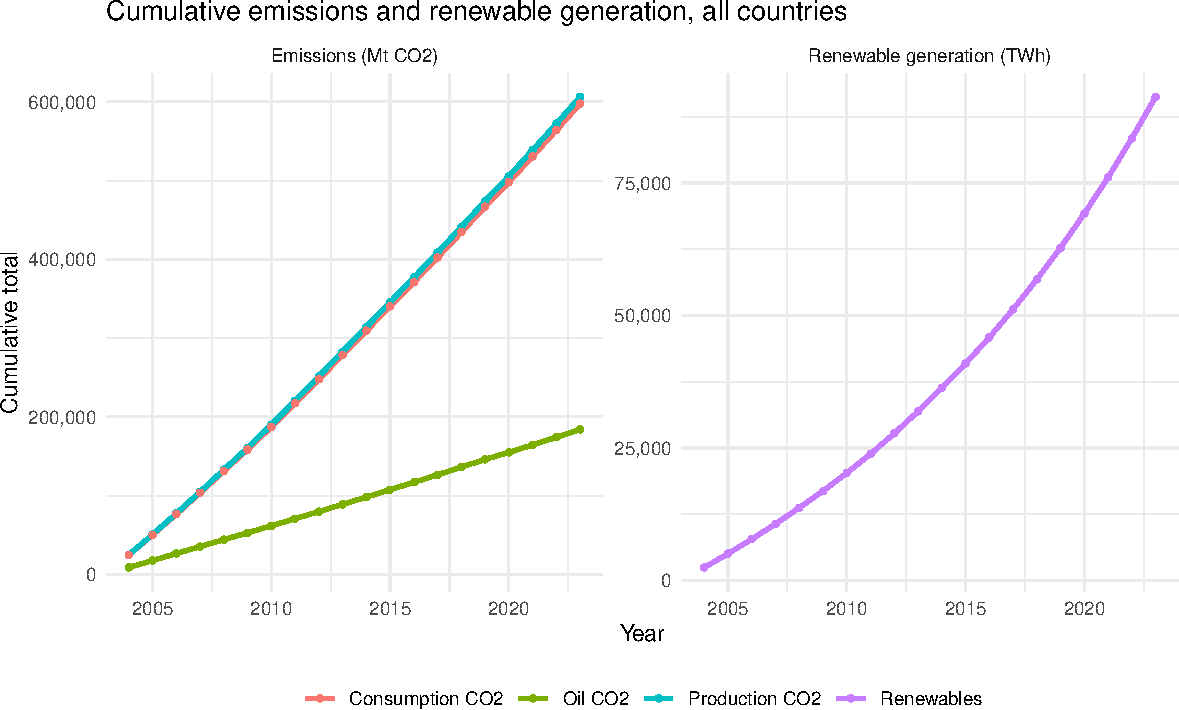
\includegraphics[keepaspectratio]{u3284342_final_assessment_files/figure-latex/t2q2-1.pdf}}

\emph{Observation:} by 2023 the 150 countries had emitted 606,423.7 Mt
of production-based CO2 since 2004, with consumption-based emissions
(597,745.8 Mt) tracking almost the same path, which is expected since
trade only moves emissions between countries. Oil accounts for 30.3\%
(184,040.5 Mt) of the total. The renewables curve bends upward, unlike
the near-straight emissions lines, showing that annual renewable
generation grew faster over the period than annual emissions.

\subsubsection{\texorpdfstring{2.3 Extract
\texttt{lastYear\_data}}{2.3 Extract lastYear\_data}}\label{extract-lastyear_data}

\emph{Compute the final year --- do not type it in.}

\begin{Shaded}
\begin{Highlighting}[]
\NormalTok{lastYear\_data }\OtherTok{\textless{}{-}}\NormalTok{ master }\SpecialCharTok{\%\textgreater{}\%} \FunctionTok{filter}\NormalTok{(Year }\SpecialCharTok{==} \FunctionTok{max}\NormalTok{(Year))}

\FunctionTok{cat}\NormalTok{(}\StringTok{"Final year:"}\NormalTok{, }\FunctionTok{unique}\NormalTok{(lastYear\_data}\SpecialCharTok{$}\NormalTok{Year), }\StringTok{"| Countries:"}\NormalTok{,}
    \FunctionTok{nrow}\NormalTok{(lastYear\_data), }\StringTok{"}\SpecialCharTok{\textbackslash{}n}\StringTok{"}\NormalTok{)}
\end{Highlighting}
\end{Shaded}

\begin{verbatim}
## Final year: 2023 | Countries: 150
\end{verbatim}

\subsubsection{2.4 Top 10 countries on four
measures}\label{top-10-countries-on-four-measures}

\emph{\texttt{top10total}, \texttt{top10percap}, \texttt{top10net},
\texttt{top10renew}.}

\begin{Shaded}
\begin{Highlighting}[]
\NormalTok{top10total }\OtherTok{\textless{}{-}}\NormalTok{ lastYear\_data }\SpecialCharTok{\%\textgreater{}\%}
  \FunctionTok{slice\_max}\NormalTok{(CumCO2, }\AttributeTok{n =} \DecValTok{10}\NormalTok{, }\AttributeTok{with\_ties =} \ConstantTok{FALSE}\NormalTok{) }\SpecialCharTok{\%\textgreater{}\%}
  \FunctionTok{select}\NormalTok{(ISO, Country, Region, CumCO2, Population, CO2\_PC)}

\NormalTok{top10percap }\OtherTok{\textless{}{-}}\NormalTok{ lastYear\_data }\SpecialCharTok{\%\textgreater{}\%}
  \FunctionTok{slice\_max}\NormalTok{(CO2\_PC, }\AttributeTok{n =} \DecValTok{10}\NormalTok{, }\AttributeTok{with\_ties =} \ConstantTok{FALSE}\NormalTok{) }\SpecialCharTok{\%\textgreater{}\%}
  \FunctionTok{select}\NormalTok{(ISO, Country, Region, CO2\_PC, CumCO2, Population)}

\NormalTok{top10net }\OtherTok{\textless{}{-}}\NormalTok{ lastYear\_data }\SpecialCharTok{\%\textgreater{}\%}
  \FunctionTok{slice\_max}\NormalTok{(NetImported, }\AttributeTok{n =} \DecValTok{10}\NormalTok{, }\AttributeTok{with\_ties =} \ConstantTok{FALSE}\NormalTok{) }\SpecialCharTok{\%\textgreater{}\%}
  \FunctionTok{select}\NormalTok{(ISO, Country, Region, NetImported, CumConsCO2, CumCO2)}

\NormalTok{top10renew }\OtherTok{\textless{}{-}}\NormalTok{ lastYear\_data }\SpecialCharTok{\%\textgreater{}\%}
  \FunctionTok{slice\_max}\NormalTok{(Renew\_PC, }\AttributeTok{n =} \DecValTok{10}\NormalTok{, }\AttributeTok{with\_ties =} \ConstantTok{FALSE}\NormalTok{) }\SpecialCharTok{\%\textgreater{}\%}
  \FunctionTok{select}\NormalTok{(ISO, Country, Region, Renew\_PC, CumRenew, Population)}

\FunctionTok{kable}\NormalTok{(top10total, }\AttributeTok{digits =} \DecValTok{1}\NormalTok{, }\AttributeTok{format.args =} \FunctionTok{list}\NormalTok{(}\AttributeTok{big.mark =} \StringTok{","}\NormalTok{),}
      \AttributeTok{caption =} \StringTok{"Top 10 by cumulative CO2 (Mt)"}\NormalTok{)}
\end{Highlighting}
\end{Shaded}

\begin{longtable}[]{@{}lllrrr@{}}
\caption{Top 10 by cumulative CO2 (Mt)}\tabularnewline
\toprule\noalign{}
ISO & Country & Region & CumCO2 & Population & CO2\_PC \\
\midrule\noalign{}
\endfirsthead
\toprule\noalign{}
ISO & Country & Region & CumCO2 & Population & CO2\_PC \\
\midrule\noalign{}
\endhead
\bottomrule\noalign{}
\endlastfoot
CHN & China & Asia & 184,474.9 & 1,425,179,562 & 129.4 \\
USA & United States & North America & 109,445.5 & 341,534,041 & 320.5 \\
IND & India & Asia & 40,844.0 & 1,425,423,209 & 28.7 \\
RUS & Russia & Europe & 32,903.1 & 145,579,889 & 226.0 \\
JPN & Japan & Asia & 23,820.7 & 124,997,585 & 190.6 \\
DEU & Germany & Europe & 15,630.9 & 84,086,227 & 185.9 \\
IRN & Iran & Asia & 12,437.8 & 89,524,247 & 138.9 \\
KOR & South Korea & Asia & 11,848.1 & 51,782,515 & 228.8 \\
SAU & Saudi Arabia & Asia & 11,495.6 & 32,175,351 & 357.3 \\
IDN & Indonesia & Asia & 10,360.2 & 278,830,527 & 37.2 \\
\end{longtable}

\begin{Shaded}
\begin{Highlighting}[]
\FunctionTok{kable}\NormalTok{(top10percap, }\AttributeTok{digits =} \DecValTok{1}\NormalTok{, }\AttributeTok{format.args =} \FunctionTok{list}\NormalTok{(}\AttributeTok{big.mark =} \StringTok{","}\NormalTok{),}
      \AttributeTok{caption =} \StringTok{"Top 10 by cumulative CO2 per capita (t)"}\NormalTok{)}
\end{Highlighting}
\end{Shaded}

\begin{longtable}[]{@{}
  >{\raggedright\arraybackslash}p{(\linewidth - 10\tabcolsep) * \real{0.0588}}
  >{\raggedright\arraybackslash}p{(\linewidth - 10\tabcolsep) * \real{0.3088}}
  >{\raggedright\arraybackslash}p{(\linewidth - 10\tabcolsep) * \real{0.2059}}
  >{\raggedleft\arraybackslash}p{(\linewidth - 10\tabcolsep) * \real{0.1029}}
  >{\raggedleft\arraybackslash}p{(\linewidth - 10\tabcolsep) * \real{0.1471}}
  >{\raggedleft\arraybackslash}p{(\linewidth - 10\tabcolsep) * \real{0.1765}}@{}}
\caption{Top 10 by cumulative CO2 per capita (t)}\tabularnewline
\toprule\noalign{}
\begin{minipage}[b]{\linewidth}\raggedright
ISO
\end{minipage} & \begin{minipage}[b]{\linewidth}\raggedright
Country
\end{minipage} & \begin{minipage}[b]{\linewidth}\raggedright
Region
\end{minipage} & \begin{minipage}[b]{\linewidth}\raggedleft
CO2\_PC
\end{minipage} & \begin{minipage}[b]{\linewidth}\raggedleft
CumCO2
\end{minipage} & \begin{minipage}[b]{\linewidth}\raggedleft
Population
\end{minipage} \\
\midrule\noalign{}
\endfirsthead
\toprule\noalign{}
\begin{minipage}[b]{\linewidth}\raggedright
ISO
\end{minipage} & \begin{minipage}[b]{\linewidth}\raggedright
Country
\end{minipage} & \begin{minipage}[b]{\linewidth}\raggedright
Region
\end{minipage} & \begin{minipage}[b]{\linewidth}\raggedleft
CO2\_PC
\end{minipage} & \begin{minipage}[b]{\linewidth}\raggedleft
CumCO2
\end{minipage} & \begin{minipage}[b]{\linewidth}\raggedleft
Population
\end{minipage} \\
\midrule\noalign{}
\endhead
\bottomrule\noalign{}
\endlastfoot
QAT & Qatar & Asia & 588.8 & 1,703.1 & 2,892,466 \\
TTO & Trinidad and Tobago & North America & 556.3 & 832.2 & 1,495,923 \\
BHR & Bahrain & Asia & 403.5 & 618.8 & 1,533,460 \\
BRN & Brunei & Asia & 389.7 & 177.4 & 455,374 \\
ARE & United Arab Emirates & Asia & 364.4 & 3,732.7 & 10,242,085 \\
SAU & Saudi Arabia & Asia & 357.3 & 11,495.6 & 32,175,351 \\
USA & United States & North America & 320.5 & 109,445.5 & 341,534,041 \\
LUX & Luxembourg & Europe & 305.7 & 199.7 & 653,315 \\
ABW & Aruba & North America & 297.4 & 32.1 & 107,792 \\
NCL & New Caledonia & Oceania & 293.4 & 84.2 & 287,130 \\
\end{longtable}

\begin{Shaded}
\begin{Highlighting}[]
\FunctionTok{kable}\NormalTok{(top10net, }\AttributeTok{digits =} \DecValTok{1}\NormalTok{, }\AttributeTok{format.args =} \FunctionTok{list}\NormalTok{(}\AttributeTok{big.mark =} \StringTok{","}\NormalTok{),}
      \AttributeTok{caption =} \StringTok{"Top 10 net importers of embodied CO2 (Mt)"}\NormalTok{)}
\end{Highlighting}
\end{Shaded}

\begin{longtable}[]{@{}
  >{\raggedright\arraybackslash}p{(\linewidth - 10\tabcolsep) * \real{0.0556}}
  >{\raggedright\arraybackslash}p{(\linewidth - 10\tabcolsep) * \real{0.2917}}
  >{\raggedright\arraybackslash}p{(\linewidth - 10\tabcolsep) * \real{0.1944}}
  >{\raggedleft\arraybackslash}p{(\linewidth - 10\tabcolsep) * \real{0.1667}}
  >{\raggedleft\arraybackslash}p{(\linewidth - 10\tabcolsep) * \real{0.1528}}
  >{\raggedleft\arraybackslash}p{(\linewidth - 10\tabcolsep) * \real{0.1389}}@{}}
\caption{Top 10 net importers of embodied CO2 (Mt)}\tabularnewline
\toprule\noalign{}
\begin{minipage}[b]{\linewidth}\raggedright
ISO
\end{minipage} & \begin{minipage}[b]{\linewidth}\raggedright
Country
\end{minipage} & \begin{minipage}[b]{\linewidth}\raggedright
Region
\end{minipage} & \begin{minipage}[b]{\linewidth}\raggedleft
NetImported
\end{minipage} & \begin{minipage}[b]{\linewidth}\raggedleft
CumConsCO2
\end{minipage} & \begin{minipage}[b]{\linewidth}\raggedleft
CumCO2
\end{minipage} \\
\midrule\noalign{}
\endfirsthead
\toprule\noalign{}
\begin{minipage}[b]{\linewidth}\raggedright
ISO
\end{minipage} & \begin{minipage}[b]{\linewidth}\raggedright
Country
\end{minipage} & \begin{minipage}[b]{\linewidth}\raggedright
Region
\end{minipage} & \begin{minipage}[b]{\linewidth}\raggedleft
NetImported
\end{minipage} & \begin{minipage}[b]{\linewidth}\raggedleft
CumConsCO2
\end{minipage} & \begin{minipage}[b]{\linewidth}\raggedleft
CumCO2
\end{minipage} \\
\midrule\noalign{}
\endhead
\bottomrule\noalign{}
\endlastfoot
USA & United States & North America & 7,062.2 & 116,507.7 & 109,445.5 \\
JPN & Japan & Asia & 3,566.0 & 27,386.6 & 23,820.7 \\
GBR & United Kingdom & Europe & 3,477.8 & 12,414.9 & 8,937.0 \\
DEU & Germany & Europe & 3,005.7 & 18,636.6 & 15,630.9 \\
FRA & France & Europe & 2,609.6 & 9,582.3 & 6,972.6 \\
ITA & Italy & Europe & 2,442.6 & 10,366.2 & 7,923.6 \\
SGP & Singapore & Asia & 2,366.7 & 3,286.8 & 920.1 \\
HKG & Hong Kong & Asia & 1,542.4 & 2,356.1 & 813.7 \\
KOR & South Korea & Asia & 1,512.7 & 13,360.8 & 11,848.1 \\
ARE & United Arab Emirates & Asia & 755.5 & 4,488.1 & 3,732.7 \\
\end{longtable}

\begin{Shaded}
\begin{Highlighting}[]
\FunctionTok{kable}\NormalTok{(top10renew, }\AttributeTok{digits =} \DecValTok{2}\NormalTok{, }\AttributeTok{format.args =} \FunctionTok{list}\NormalTok{(}\AttributeTok{big.mark =} \StringTok{","}\NormalTok{),}
      \AttributeTok{caption =} \StringTok{"Top 10 by renewables per capita (TWh per million people)"}\NormalTok{)}
\end{Highlighting}
\end{Shaded}

\begin{longtable}[]{@{}lllrrr@{}}
\caption{Top 10 by renewables per capita (TWh per million
people)}\tabularnewline
\toprule\noalign{}
ISO & Country & Region & Renew\_PC & CumRenew & Population \\
\midrule\noalign{}
\endfirsthead
\toprule\noalign{}
ISO & Country & Region & Renew\_PC & CumRenew & Population \\
\midrule\noalign{}
\endhead
\bottomrule\noalign{}
\endlastfoot
ISL & Iceland & Europe & 871.29 & 331.41 & 380,368 \\
NOR & Norway & Europe & 499.84 & 2,727.54 & 5,456,796 \\
BTN & Bhutan & Asia & 189.90 & 148.30 & 780,921 \\
SWE & Sweden & Europe & 174.51 & 1,830.19 & 10,487,335 \\
NZL & New Zealand & Oceania & 128.93 & 661.63 & 5,131,731 \\
GRL & Greenland & North America & 122.11 & 6.84 & 56,014 \\
AUT & Austria & Europe & 106.69 & 967.13 & 9,064,678 \\
FIN & Finland & Europe & 105.16 & 585.67 & 5,569,300 \\
URY & Uruguay & South America & 59.83 & 202.87 & 3,390,913 \\
DNK & Denmark & Europe & 58.37 & 344.58 & 5,902,901 \\
\end{longtable}

\subsubsection{2.5 Totals by region}\label{totals-by-region}

\begin{Shaded}
\begin{Highlighting}[]
\NormalTok{region\_totals }\OtherTok{\textless{}{-}}\NormalTok{ lastYear\_data }\SpecialCharTok{\%\textgreater{}\%}
  \FunctionTok{group\_by}\NormalTok{(Region) }\SpecialCharTok{\%\textgreater{}\%}
  \FunctionTok{summarise}\NormalTok{(}\AttributeTok{Countries =} \FunctionTok{n}\NormalTok{(),}
            \AttributeTok{CumCO2 =} \FunctionTok{sum}\NormalTok{(CumCO2),}
            \AttributeTok{CumOilCO2 =} \FunctionTok{sum}\NormalTok{(CumOilCO2),}
            \AttributeTok{CumRenew =} \FunctionTok{sum}\NormalTok{(CumRenew),}
            \AttributeTok{CumConsCO2 =} \FunctionTok{sum}\NormalTok{(CumConsCO2),}
            \AttributeTok{.groups =} \StringTok{"drop"}\NormalTok{) }\SpecialCharTok{\%\textgreater{}\%}
  \FunctionTok{arrange}\NormalTok{(}\FunctionTok{desc}\NormalTok{(CumCO2))}

\FunctionTok{kable}\NormalTok{(region\_totals, }\AttributeTok{digits =} \DecValTok{1}\NormalTok{, }\AttributeTok{format.args =} \FunctionTok{list}\NormalTok{(}\AttributeTok{big.mark =} \StringTok{","}\NormalTok{),}
      \AttributeTok{caption =} \StringTok{"Cumulative totals by region (CO2 in Mt, renewables in TWh)"}\NormalTok{)}
\end{Highlighting}
\end{Shaded}

\begin{longtable}[]{@{}lrrrrr@{}}
\caption{Cumulative totals by region (CO2 in Mt, renewables in
TWh)}\tabularnewline
\toprule\noalign{}
Region & Countries & CumCO2 & CumOilCO2 & CumRenew & CumConsCO2 \\
\midrule\noalign{}
\endfirsthead
\toprule\noalign{}
Region & Countries & CumCO2 & CumOilCO2 & CumRenew & CumConsCO2 \\
\midrule\noalign{}
\endhead
\bottomrule\noalign{}
\endlastfoot
Asia & 39 & 345,927.5 & 81,256.4 & 40,331.9 & 323,929.9 \\
North America & 22 & 112,422.3 & 47,685.9 & 12,364.8 & 119,559.3 \\
Europe & 33 & 102,564.4 & 33,841.5 & 21,543.5 & 109,687.0 \\
Africa & 41 & 23,825.1 & 8,339.5 & 2,363.4 & 22,574.0 \\
South America & 10 & 20,729.6 & 12,344.6 & 13,963.1 & 20,920.3 \\
Oceania & 5 & 954.8 & 572.6 & 710.5 & 1,075.3 \\
\end{longtable}

\emph{Observation:} Asia accounts for 345,927.5 Mt, 57\% of all
cumulative emissions, and is the only region where consumption-based
emissions (323,929.9 Mt) fall well below production, making it a net
exporter of embodied carbon. Europe and North America are net importers:
Europe consumed 109,687.0 Mt against 102,564.4 Mt produced. South
America stands out for renewables, with 13,963.1 TWh against only
20,729.6 Mt of CO2.

\subsubsection{2.6 Cumulative emissions over time, top 10 countries (log
Y)}\label{cumulative-emissions-over-time-top-10-countries-log-y}

\begin{Shaded}
\begin{Highlighting}[]
\NormalTok{top10\_series }\OtherTok{\textless{}{-}}\NormalTok{ master }\SpecialCharTok{\%\textgreater{}\%} \FunctionTok{filter}\NormalTok{(ISO }\SpecialCharTok{\%in\%}\NormalTok{ top10total}\SpecialCharTok{$}\NormalTok{ISO)}
\NormalTok{top10\_labels }\OtherTok{\textless{}{-}}\NormalTok{ top10\_series }\SpecialCharTok{\%\textgreater{}\%} \FunctionTok{filter}\NormalTok{(Year }\SpecialCharTok{==} \FunctionTok{max}\NormalTok{(Year))}

\FunctionTok{ggplot}\NormalTok{(top10\_series, }\FunctionTok{aes}\NormalTok{(Year, CumCO2, }\AttributeTok{colour =}\NormalTok{ Country)) }\SpecialCharTok{+}
  \FunctionTok{geom\_line}\NormalTok{(}\AttributeTok{linewidth =} \FloatTok{0.9}\NormalTok{) }\SpecialCharTok{+}
  \CommentTok{\# Labels at the line ends replace a 10{-}colour legend lookup.}
  \FunctionTok{geom\_text}\NormalTok{(}\AttributeTok{data =}\NormalTok{ top10\_labels, }\FunctionTok{aes}\NormalTok{(}\AttributeTok{label =}\NormalTok{ Country), }\AttributeTok{hjust =} \SpecialCharTok{{-}}\FloatTok{0.1}\NormalTok{,}
            \AttributeTok{size =} \DecValTok{3}\NormalTok{, }\AttributeTok{show.legend =} \ConstantTok{FALSE}\NormalTok{) }\SpecialCharTok{+}
  \FunctionTok{scale\_y\_log10}\NormalTok{(}\AttributeTok{labels =} \FunctionTok{label\_comma}\NormalTok{()) }\SpecialCharTok{+}
  \FunctionTok{scale\_x\_continuous}\NormalTok{(}\AttributeTok{breaks =} \FunctionTok{seq}\NormalTok{(}\DecValTok{2005}\NormalTok{, }\DecValTok{2020}\NormalTok{, }\DecValTok{5}\NormalTok{),}
                     \AttributeTok{expand =} \FunctionTok{expansion}\NormalTok{(}\AttributeTok{mult =} \FunctionTok{c}\NormalTok{(}\FloatTok{0.02}\NormalTok{, }\FloatTok{0.2}\NormalTok{))) }\SpecialCharTok{+}
  \FunctionTok{labs}\NormalTok{(}\AttributeTok{title =} \StringTok{"Cumulative CO2 emissions, top 10 countries"}\NormalTok{,}
       \AttributeTok{subtitle =} \StringTok{"Log scale: equal vertical distances are equal ratios"}\NormalTok{,}
       \AttributeTok{x =} \StringTok{"Year"}\NormalTok{, }\AttributeTok{y =} \StringTok{"Cumulative CO2 (Mt, log scale)"}\NormalTok{) }\SpecialCharTok{+}
  \FunctionTok{theme}\NormalTok{(}\AttributeTok{legend.position =} \StringTok{"none"}\NormalTok{)}
\end{Highlighting}
\end{Shaded}

\pandocbounded{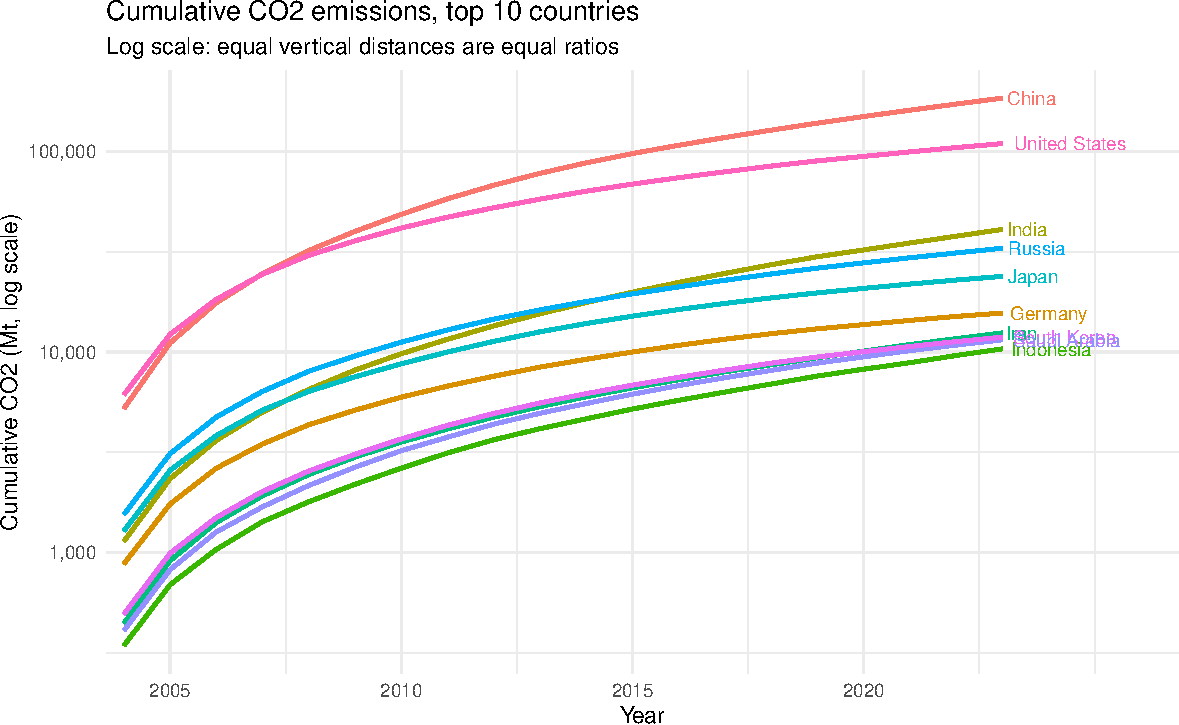
\includegraphics[keepaspectratio]{u3284342_final_assessment_files/figure-latex/t2q6-1.pdf}}

\emph{Observation:} China (184,474.9 Mt) and the United States
(109,445.5 Mt) are far ahead of the rest; China's line overtakes the
United States' around 2007. India's line keeps a steeper slope than
Japan's and Russia's, so it overtook both during the period. The steep
rise in the first years is the running total starting in 2004, not a
surge in emissions.

\subsubsection{2.7 Faceted plot, one panel per
country}\label{faceted-plot-one-panel-per-country}

\begin{Shaded}
\begin{Highlighting}[]
\NormalTok{top10\_annual }\OtherTok{\textless{}{-}}\NormalTok{ master }\SpecialCharTok{\%\textgreater{}\%}
  \FunctionTok{filter}\NormalTok{(ISO }\SpecialCharTok{\%in\%}\NormalTok{ top10total}\SpecialCharTok{$}\NormalTok{ISO) }\SpecialCharTok{\%\textgreater{}\%}
  \FunctionTok{select}\NormalTok{(Country, Year, CO2, OilCO2, Renewables) }\SpecialCharTok{\%\textgreater{}\%}
  \FunctionTok{pivot\_longer}\NormalTok{(}\FunctionTok{c}\NormalTok{(CO2, OilCO2, Renewables), }\AttributeTok{names\_to =} \StringTok{"Variable"}\NormalTok{,}
               \AttributeTok{values\_to =} \StringTok{"Value"}\NormalTok{) }\SpecialCharTok{\%\textgreater{}\%}
  \FunctionTok{mutate}\NormalTok{(}\AttributeTok{Variable =} \FunctionTok{recode}\NormalTok{(Variable, }\AttributeTok{CO2 =} \StringTok{"Annual CO2 (Mt)"}\NormalTok{,}
                           \AttributeTok{OilCO2 =} \StringTok{"Annual oil CO2 (Mt)"}\NormalTok{,}
                           \AttributeTok{Renewables =} \StringTok{"Renewable generation (TWh)"}\NormalTok{),}
         \AttributeTok{Country =} \FunctionTok{fct\_reorder}\NormalTok{(Country, Value, }\AttributeTok{.fun =}\NormalTok{ max, }\AttributeTok{.desc =} \ConstantTok{TRUE}\NormalTok{))}

\FunctionTok{ggplot}\NormalTok{(top10\_annual, }\FunctionTok{aes}\NormalTok{(Year, Value, }\AttributeTok{colour =}\NormalTok{ Variable)) }\SpecialCharTok{+}
  \FunctionTok{geom\_line}\NormalTok{(}\AttributeTok{linewidth =} \FloatTok{0.8}\NormalTok{) }\SpecialCharTok{+}
  \FunctionTok{facet\_wrap}\NormalTok{(}\SpecialCharTok{\textasciitilde{}}\NormalTok{ Country, }\AttributeTok{ncol =} \DecValTok{5}\NormalTok{, }\AttributeTok{scales =} \StringTok{"free\_y"}\NormalTok{) }\SpecialCharTok{+}
  \FunctionTok{scale\_colour\_manual}\NormalTok{(}\AttributeTok{values =} \FunctionTok{c}\NormalTok{(}\StringTok{"\#B2182B"}\NormalTok{, }\StringTok{"\#EF8A62"}\NormalTok{, }\StringTok{"\#1B7837"}\NormalTok{)) }\SpecialCharTok{+}
  \FunctionTok{scale\_y\_continuous}\NormalTok{(}\AttributeTok{labels =} \FunctionTok{label\_comma}\NormalTok{()) }\SpecialCharTok{+}
  \FunctionTok{labs}\NormalTok{(}\AttributeTok{title =} \StringTok{"Annual CO2, oil CO2 and renewable generation, top 10 emitters"}\NormalTok{,}
       \AttributeTok{subtitle =} \StringTok{"Each panel has its own y{-}axis"}\NormalTok{,}
       \AttributeTok{x =} \StringTok{"Year"}\NormalTok{, }\AttributeTok{y =} \StringTok{"Mt CO2 / TWh"}\NormalTok{, }\AttributeTok{colour =} \ConstantTok{NULL}\NormalTok{) }\SpecialCharTok{+}
  \FunctionTok{theme}\NormalTok{(}\AttributeTok{legend.position =} \StringTok{"bottom"}\NormalTok{,}
        \AttributeTok{axis.text.x =} \FunctionTok{element\_text}\NormalTok{(}\AttributeTok{angle =} \DecValTok{45}\NormalTok{, }\AttributeTok{hjust =} \DecValTok{1}\NormalTok{))}
\end{Highlighting}
\end{Shaded}

\pandocbounded{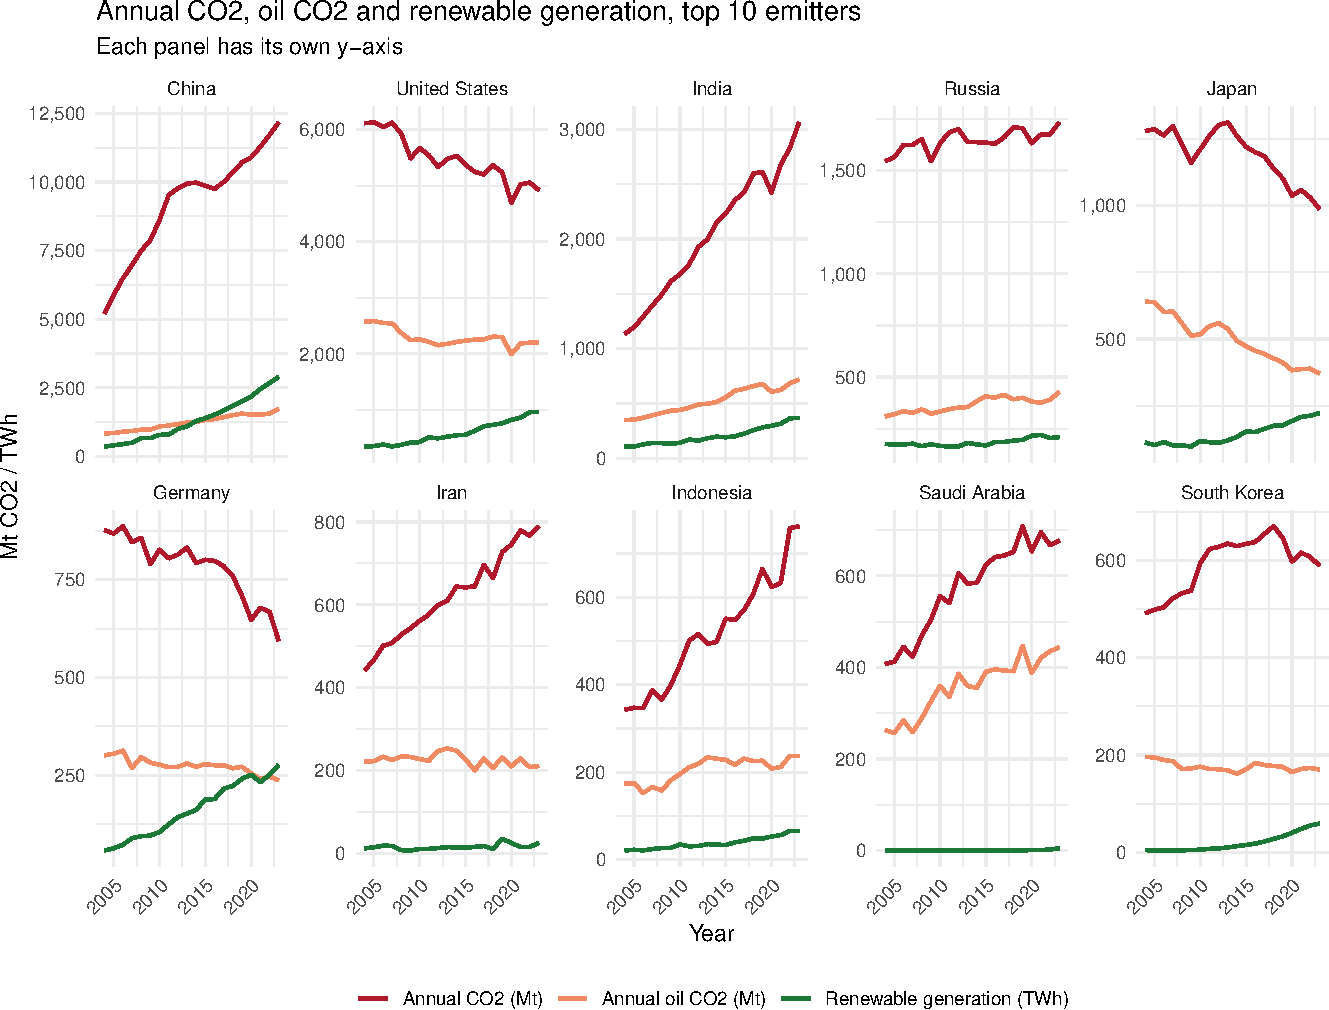
\includegraphics[keepaspectratio]{u3284342_final_assessment_files/figure-latex/t2q7-1.pdf}}

\emph{Observation:} the panels split into two groups. In the United
States, Japan and Germany annual CO2 declines while renewable generation
rises (Germany's from 57.97 TWh in 2004 to 277.1 TWh in 2023). In China,
India, Indonesia, Iran and Saudi Arabia emissions keep climbing; China's
renewables grow fastest of all (357.43 to 2,894.22 TWh) but not fast
enough to bend its emissions curve, and Saudi Arabia's renewable
generation stays close to zero.

\subsubsection{2.8 Top 10 by emissions per
capita}\label{top-10-by-emissions-per-capita}

\begin{Shaded}
\begin{Highlighting}[]
\NormalTok{percap\_long }\OtherTok{\textless{}{-}}\NormalTok{ top10percap }\SpecialCharTok{\%\textgreater{}\%}
  \FunctionTok{transmute}\NormalTok{(}\AttributeTok{Country =} \FunctionTok{fct\_reorder}\NormalTok{(Country, CO2\_PC),}
            \StringTok{\textasciigrave{}}\AttributeTok{Cumulative CO2 (Mt)}\StringTok{\textasciigrave{}} \OtherTok{=}\NormalTok{ CumCO2,}
            \StringTok{\textasciigrave{}}\AttributeTok{Population (millions)}\StringTok{\textasciigrave{}} \OtherTok{=}\NormalTok{ Population }\SpecialCharTok{/} \FloatTok{1e6}\NormalTok{,}
            \StringTok{\textasciigrave{}}\AttributeTok{Cumulative CO2 per capita (t)}\StringTok{\textasciigrave{}} \OtherTok{=}\NormalTok{ CO2\_PC) }\SpecialCharTok{\%\textgreater{}\%}
  \FunctionTok{pivot\_longer}\NormalTok{(}\SpecialCharTok{{-}}\NormalTok{Country, }\AttributeTok{names\_to =} \StringTok{"Measure"}\NormalTok{, }\AttributeTok{values\_to =} \StringTok{"Value"}\NormalTok{) }\SpecialCharTok{\%\textgreater{}\%}
  \FunctionTok{mutate}\NormalTok{(}\AttributeTok{Measure =} \FunctionTok{factor}\NormalTok{(Measure, }\AttributeTok{levels =} \FunctionTok{c}\NormalTok{(}
    \StringTok{"Cumulative CO2 per capita (t)"}\NormalTok{, }\StringTok{"Cumulative CO2 (Mt)"}\NormalTok{,}
    \StringTok{"Population (millions)"}\NormalTok{)))}

\FunctionTok{ggplot}\NormalTok{(percap\_long, }\FunctionTok{aes}\NormalTok{(Value, Country, }\AttributeTok{fill =}\NormalTok{ Measure)) }\SpecialCharTok{+}
  \FunctionTok{geom\_col}\NormalTok{(}\AttributeTok{show.legend =} \ConstantTok{FALSE}\NormalTok{) }\SpecialCharTok{+}
  \FunctionTok{facet\_wrap}\NormalTok{(}\SpecialCharTok{\textasciitilde{}}\NormalTok{ Measure, }\AttributeTok{scales =} \StringTok{"free\_x"}\NormalTok{) }\SpecialCharTok{+}
  \FunctionTok{scale\_x\_continuous}\NormalTok{(}\AttributeTok{labels =} \FunctionTok{label\_comma}\NormalTok{()) }\SpecialCharTok{+}
  \FunctionTok{labs}\NormalTok{(}\AttributeTok{title =} \StringTok{"Top 10 countries by cumulative CO2 per capita"}\NormalTok{,}
       \AttributeTok{subtitle =} \StringTok{"Countries ordered by per{-}capita emissions"}\NormalTok{,}
       \AttributeTok{x =} \ConstantTok{NULL}\NormalTok{, }\AttributeTok{y =} \ConstantTok{NULL}\NormalTok{)}
\end{Highlighting}
\end{Shaded}

\pandocbounded{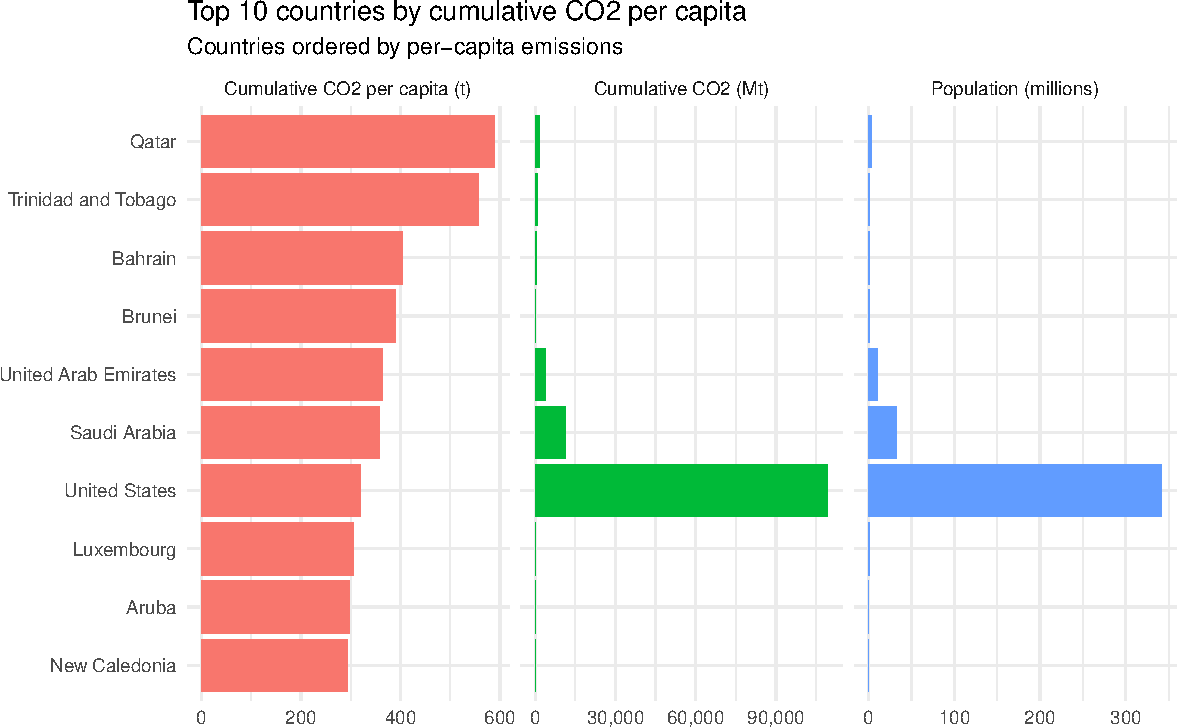
\includegraphics[keepaspectratio]{u3284342_final_assessment_files/figure-latex/t2q8-1.pdf}}

\subsubsection{2.9 Total, average and median cumulative emissions by
region}\label{total-average-and-median-cumulative-emissions-by-region}

\begin{Shaded}
\begin{Highlighting}[]
\NormalTok{region\_stats }\OtherTok{\textless{}{-}}\NormalTok{ lastYear\_data }\SpecialCharTok{\%\textgreater{}\%}
  \FunctionTok{group\_by}\NormalTok{(Region) }\SpecialCharTok{\%\textgreater{}\%}
  \FunctionTok{summarise}\NormalTok{(}\AttributeTok{Total =} \FunctionTok{sum}\NormalTok{(CumCO2), }\AttributeTok{Average =} \FunctionTok{mean}\NormalTok{(CumCO2),}
            \AttributeTok{Median =} \FunctionTok{median}\NormalTok{(CumCO2), }\AttributeTok{.groups =} \StringTok{"drop"}\NormalTok{) }\SpecialCharTok{\%\textgreater{}\%}
  \FunctionTok{pivot\_longer}\NormalTok{(}\SpecialCharTok{{-}}\NormalTok{Region, }\AttributeTok{names\_to =} \StringTok{"Statistic"}\NormalTok{, }\AttributeTok{values\_to =} \StringTok{"Value"}\NormalTok{) }\SpecialCharTok{\%\textgreater{}\%}
  \FunctionTok{mutate}\NormalTok{(}\AttributeTok{Statistic =} \FunctionTok{factor}\NormalTok{(Statistic,}
                            \AttributeTok{levels =} \FunctionTok{c}\NormalTok{(}\StringTok{"Total"}\NormalTok{, }\StringTok{"Average"}\NormalTok{, }\StringTok{"Median"}\NormalTok{)))}

\FunctionTok{ggplot}\NormalTok{(region\_stats, }\FunctionTok{aes}\NormalTok{(Region, Value, }\AttributeTok{fill =}\NormalTok{ Region)) }\SpecialCharTok{+}
  \FunctionTok{geom\_col}\NormalTok{() }\SpecialCharTok{+}
  \FunctionTok{facet\_wrap}\NormalTok{(}\SpecialCharTok{\textasciitilde{}}\NormalTok{ Statistic, }\AttributeTok{scales =} \StringTok{"free\_y"}\NormalTok{) }\SpecialCharTok{+}
  \FunctionTok{scale\_y\_continuous}\NormalTok{(}\AttributeTok{labels =} \FunctionTok{label\_comma}\NormalTok{()) }\SpecialCharTok{+}
  \FunctionTok{labs}\NormalTok{(}\AttributeTok{title =} \StringTok{"Cumulative CO2 by region: total, average and median"}\NormalTok{,}
       \AttributeTok{x =} \ConstantTok{NULL}\NormalTok{, }\AttributeTok{y =} \StringTok{"Cumulative CO2 (Mt)"}\NormalTok{, }\AttributeTok{fill =} \StringTok{"Region"}\NormalTok{) }\SpecialCharTok{+}
  \FunctionTok{theme}\NormalTok{(}\AttributeTok{axis.text.x =} \FunctionTok{element\_text}\NormalTok{(}\AttributeTok{angle =} \DecValTok{45}\NormalTok{, }\AttributeTok{hjust =} \DecValTok{1}\NormalTok{))}
\end{Highlighting}
\end{Shaded}

\pandocbounded{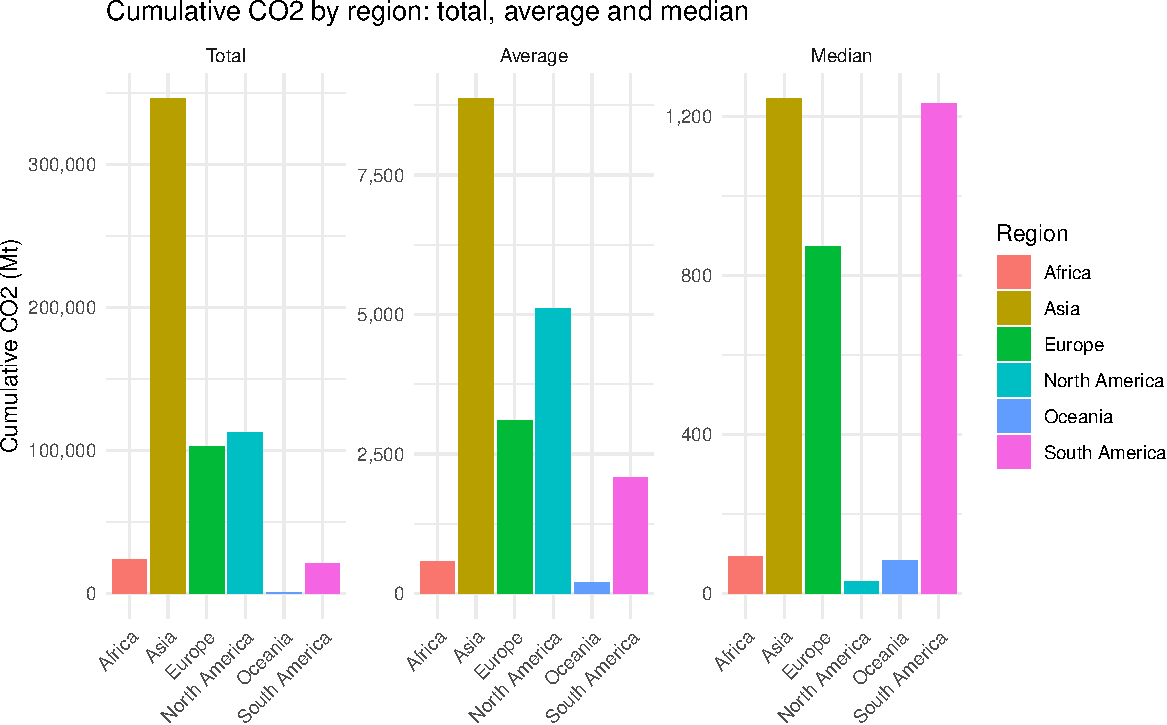
\includegraphics[keepaspectratio]{u3284342_final_assessment_files/figure-latex/t2q9-1.pdf}}

\emph{Observation:} comparing the three panels shows how skewed each
region is. North America has the second-highest average (about 5,100 Mt)
but one of the lowest medians, because the United States (109,445.5 Mt)
dominates 22 mostly small countries. South America's median (about 1,230
Mt) almost matches Asia's despite a far smaller total, because its 10
countries are mostly mid-sized emitters with no single giant.

\subsubsection{2.10 Top 2 countries per region by emissions per
capita}\label{top-2-countries-per-region-by-emissions-per-capita}

\begin{Shaded}
\begin{Highlighting}[]
\NormalTok{top2\_region }\OtherTok{\textless{}{-}}\NormalTok{ lastYear\_data }\SpecialCharTok{\%\textgreater{}\%}
  \FunctionTok{group\_by}\NormalTok{(Region) }\SpecialCharTok{\%\textgreater{}\%}
  \FunctionTok{slice\_max}\NormalTok{(CO2\_PC, }\AttributeTok{n =} \DecValTok{2}\NormalTok{, }\AttributeTok{with\_ties =} \ConstantTok{FALSE}\NormalTok{) }\SpecialCharTok{\%\textgreater{}\%}
  \FunctionTok{ungroup}\NormalTok{() }\SpecialCharTok{\%\textgreater{}\%}
  \FunctionTok{select}\NormalTok{(Region, Country, CO2\_PC, CumCO2, Population) }\SpecialCharTok{\%\textgreater{}\%}
  \FunctionTok{arrange}\NormalTok{(Region, }\FunctionTok{desc}\NormalTok{(CO2\_PC))}

\FunctionTok{kable}\NormalTok{(top2\_region, }\AttributeTok{digits =} \DecValTok{1}\NormalTok{, }\AttributeTok{format.args =} \FunctionTok{list}\NormalTok{(}\AttributeTok{big.mark =} \StringTok{","}\NormalTok{),}
      \AttributeTok{caption =} \StringTok{"Top 2 countries per region by cumulative CO2 per capita (t)"}\NormalTok{)}
\end{Highlighting}
\end{Shaded}

\begin{longtable}[]{@{}llrrr@{}}
\caption{Top 2 countries per region by cumulative CO2 per capita
(t)}\tabularnewline
\toprule\noalign{}
Region & Country & CO2\_PC & CumCO2 & Population \\
\midrule\noalign{}
\endfirsthead
\toprule\noalign{}
Region & Country & CO2\_PC & CumCO2 & Population \\
\midrule\noalign{}
\endhead
\bottomrule\noalign{}
\endlastfoot
Africa & Libya & 158.0 & 1,141.4 & 7,223,804 \\
Africa & South Africa & 146.0 & 9,106.6 & 62,378,417 \\
Asia & Qatar & 588.8 & 1,703.1 & 2,892,466 \\
Asia & Bahrain & 403.5 & 618.8 & 1,533,460 \\
Europe & Luxembourg & 305.7 & 199.7 & 653,315 \\
Europe & Estonia & 236.5 & 319.3 & 1,350,093 \\
North America & Trinidad and Tobago & 556.3 & 832.2 & 1,495,923 \\
North America & United States & 320.5 & 109,445.5 & 341,534,041 \\
Oceania & New Caledonia & 293.4 & 84.2 & 287,130 \\
Oceania & New Zealand & 137.3 & 704.8 & 5,131,731 \\
South America & Venezuela & 102.7 & 2,896.4 & 28,213,015 \\
South America & Argentina & 79.9 & 3,627.6 & 45,407,904 \\
\end{longtable}

\begin{center}\rule{0.5\linewidth}{0.5pt}\end{center}

\subsection{2A. Counterintuitive
finding}\label{a.-counterintuitive-finding}

\emph{What did you expect, and why was that reasonable?}

I expected the countries with the largest cumulative emissions to also
lead the per-capita ranking, and expected any per-capita leaders outside
that group to be oil-dominated economies. This was reasonable because a
handful of large industrial economies dominate the totals (China alone
emitted 184,474.9 Mt, 30\% of the sample), and oil is the fuel most
associated with high-consumption lifestyles and petro-states.

\emph{What does the data actually show? Quote a specific value, country
or trend from your own plots.}

Only two countries, the United States (320.5 t per person) and Saudi
Arabia (357.3 t), appear in both \texttt{top10total} and
\texttt{top10percap}. The per-capita leader is Qatar at 588.8 t per
person, 4.5 times China's 129.4 t and 20 times India's 28.7 t, despite
having just 2.9 million people and a cumulative total (1,703.1 Mt) under
1\% of China's. Only 3 of the top 10 per-capita countries have more than
10 million people. The supporting chart also contradicts the second half
of my expectation: Qatar, Bahrain, Brunei and the United Arab Emirates
sit at the top-left in dark colours, meaning oil makes up under a
quarter of their cumulative emissions, while the oil-dominated (yellow)
points are mostly small island economies such as Aruba.

\emph{What real-world mechanism could explain the discrepancy?}

Two mechanisms combine. The first is population size: per-capita
emissions divide a country's total by its population, so a country with
fewer than 3 million people needs only a modest industrial base to post
a very high figure. The second is energy resource endowment combined
with production-based accounting. Qatar, Bahrain, Brunei and the UAE are
natural-gas exporters: liquefying and processing gas, refining,
petrochemicals and energy-intensive industries such as aluminium
smelting, all powered by cheap domestic gas, emit CO2 inside their
borders, even though much of the output is exported and consumed
elsewhere. Production-based accounting assigns all of those emissions to
a small resident population, which is why gas, not oil, drives the
highest per-capita figures.

\subsubsection{Supporting visualisation}\label{supporting-visualisation}

\begin{Shaded}
\begin{Highlighting}[]
\CommentTok{\# Population vs per{-}capita emissions, coloured by oil share: tests whether}
\CommentTok{\# the per{-}capita leaders are small, oil{-} or gas{-}intensive economies rather}
\CommentTok{\# than the large total emitters.}
\NormalTok{label\_iso }\OtherTok{\textless{}{-}} \FunctionTok{union}\NormalTok{(top10total}\SpecialCharTok{$}\NormalTok{ISO, top10percap}\SpecialCharTok{$}\NormalTok{ISO)}

\FunctionTok{ggplot}\NormalTok{(lastYear\_data, }\FunctionTok{aes}\NormalTok{(Population }\SpecialCharTok{/} \FloatTok{1e6}\NormalTok{, CO2\_PC)) }\SpecialCharTok{+}
  \FunctionTok{geom\_point}\NormalTok{(}\FunctionTok{aes}\NormalTok{(}\AttributeTok{size =}\NormalTok{ CumCO2, }\AttributeTok{colour =}\NormalTok{ OilShare), }\AttributeTok{alpha =} \FloatTok{0.75}\NormalTok{) }\SpecialCharTok{+}
  \FunctionTok{geom\_text}\NormalTok{(}\AttributeTok{data =} \FunctionTok{filter}\NormalTok{(lastYear\_data, ISO }\SpecialCharTok{\%in\%}\NormalTok{ label\_iso),}
            \FunctionTok{aes}\NormalTok{(}\AttributeTok{label =}\NormalTok{ Country), }\AttributeTok{size =} \FloatTok{2.8}\NormalTok{, }\AttributeTok{vjust =} \SpecialCharTok{{-}}\FloatTok{0.9}\NormalTok{,}
            \AttributeTok{check\_overlap =} \ConstantTok{TRUE}\NormalTok{) }\SpecialCharTok{+}
  \FunctionTok{scale\_x\_log10}\NormalTok{(}\AttributeTok{labels =} \FunctionTok{label\_comma}\NormalTok{()) }\SpecialCharTok{+}
  \FunctionTok{scale\_y\_log10}\NormalTok{(}\AttributeTok{labels =} \FunctionTok{label\_comma}\NormalTok{()) }\SpecialCharTok{+}
  \FunctionTok{scale\_colour\_viridis\_c}\NormalTok{(}\AttributeTok{labels =} \FunctionTok{label\_percent}\NormalTok{()) }\SpecialCharTok{+}
  \FunctionTok{scale\_size\_continuous}\NormalTok{(}\AttributeTok{labels =} \FunctionTok{label\_comma}\NormalTok{(), }\AttributeTok{range =} \FunctionTok{c}\NormalTok{(}\DecValTok{1}\NormalTok{, }\DecValTok{10}\NormalTok{)) }\SpecialCharTok{+}
  \FunctionTok{labs}\NormalTok{(}\AttributeTok{title =} \StringTok{"Small populations, high per{-}capita emissions"}\NormalTok{,}
       \AttributeTok{x =} \StringTok{"Population (millions, log scale)"}\NormalTok{,}
       \AttributeTok{y =} \StringTok{"Cumulative CO2 per capita (t, log scale)"}\NormalTok{,}
       \AttributeTok{colour =} \StringTok{"Oil share"}\NormalTok{, }\AttributeTok{size =} \StringTok{"Cumulative CO2 (Mt)"}\NormalTok{)}
\end{Highlighting}
\end{Shaded}

\pandocbounded{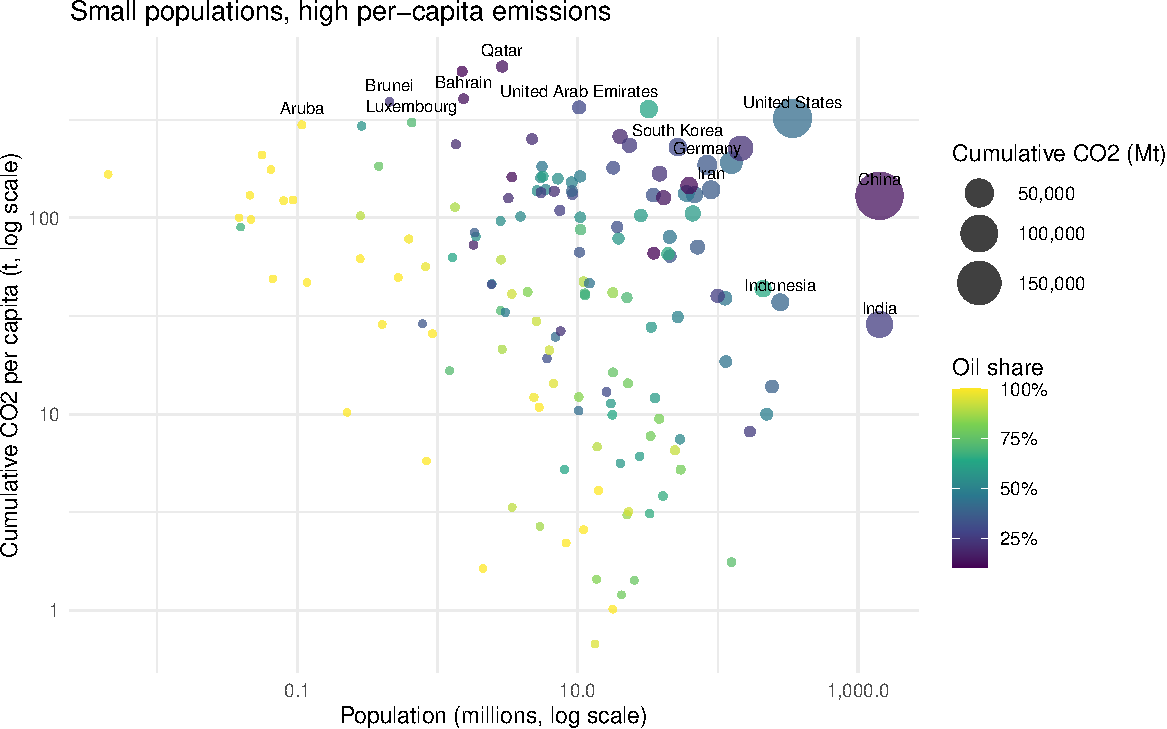
\includegraphics[keepaspectratio]{u3284342_final_assessment_files/figure-latex/t2a-plot-1.pdf}}

\emph{Caption (2--3 sentences): what does this chart show, and why did
you choose this chart type?}

Each point is one country in 2023, placed by population and cumulative
CO2 per person, with bubble size showing its cumulative total and colour
its oil share. The per-capita leaders cluster at the top-left (small
populations), while the largest total emitters (the biggest bubbles,
China and India) sit at the right with moderate per-capita values. I
chose a scatter plot with log axes because population ranges from
thousands to 1.4 billion and per-capita emissions from under 1 to 589 t,
and size and colour let one chart test both parts of the explanation.

\begin{center}\rule{0.5\linewidth}{0.5pt}\end{center}

\subsection{2B. Visualisation design
critique}\label{b.-visualisation-design-critique}

\textbf{Visualisation chosen:} Question 2.6, cumulative CO2 over time
for the top 10 countries (log y-axis).

The first design decision was the log scale. Cumulative totals range
from 10,360.2 Mt (Indonesia) to 184,474.9 Mt (China); on a log axis,
equal vertical distances are equal ratios, so all ten growth paths are
readable and comparable. The second was labelling each line at its end
instead of using a legend, so a reader does not have to match ten
colours. I rejected a linear y-axis: China and the United States would
fill the plot while the other eight countries collapsed into an
indistinguishable band near zero, hiding the fact that India overtook
Japan and Russia, which matters to a climate-policy audience tracking
emerging emitters. The limitation is that the log scale shrinks gaps:
China's lead over Indonesia is about 18 times, but the lines look close.
A reader could also mistake the steep early rise for an emissions surge
when it is the running total starting in 2004. I would mitigate both
with an annotation stating the ratio and a subtitle explaining that the
totals start in 2004.

\newpage

\section{Task 3: Data-driven
modelling}\label{task-3-data-driven-modelling}

\subsubsection{\texorpdfstring{3.1 Build
\texttt{cor\_data}}{3.1 Build cor\_data}}\label{build-cor_data}

\begin{Shaded}
\begin{Highlighting}[]
\CommentTok{\# Final{-}year record for each country (each country\textquotesingle{}s own last year, in}
\CommentTok{\# case a country\textquotesingle{}s record ends early). Country names are kept as row}
\CommentTok{\# names so the diagnostic plots in 3A label points by country.}
\NormalTok{cor\_data }\OtherTok{\textless{}{-}}\NormalTok{ master }\SpecialCharTok{\%\textgreater{}\%}
  \FunctionTok{group\_by}\NormalTok{(ISO) }\SpecialCharTok{\%\textgreater{}\%}
  \FunctionTok{filter}\NormalTok{(Year }\SpecialCharTok{==} \FunctionTok{max}\NormalTok{(Year)) }\SpecialCharTok{\%\textgreater{}\%}
  \FunctionTok{ungroup}\NormalTok{() }\SpecialCharTok{\%\textgreater{}\%}
  \FunctionTok{select}\NormalTok{(Country, CumCO2, CumConsCO2, Population, GDP, GDPCapita) }\SpecialCharTok{\%\textgreater{}\%}
  \FunctionTok{column\_to\_rownames}\NormalTok{(}\StringTok{"Country"}\NormalTok{) }\SpecialCharTok{\%\textgreater{}\%}
  \FunctionTok{as.data.frame}\NormalTok{()}

\FunctionTok{dim}\NormalTok{(cor\_data)}
\end{Highlighting}
\end{Shaded}

\begin{verbatim}
## [1] 150   5
\end{verbatim}

\begin{Shaded}
\begin{Highlighting}[]
\FunctionTok{head}\NormalTok{(cor\_data)}
\end{Highlighting}
\end{Shaded}

\begin{verbatim}
##                        CumCO2 CumConsCO2 Population        GDP GDPCapita
## Aruba                  32.053     32.053     107792   1194.874     11085
## Afghanistan           155.390    155.390   40578847  53303.000      1314
## Angola                431.269    431.269   35635028 158346.000      4444
## Albania                95.175    123.165    2827614  36171.000     12792
## Andorra                 9.749      9.749      79722   2263.068     28387
## United Arab Emirates 3732.660   4488.128   10242085 779702.000     76127
\end{verbatim}

\subsubsection{3.2 Correlation matrix}\label{correlation-matrix}

\begin{Shaded}
\begin{Highlighting}[]
\NormalTok{cor\_matrix }\OtherTok{\textless{}{-}} \FunctionTok{cor}\NormalTok{(cor\_data)}
\FunctionTok{round}\NormalTok{(cor\_matrix, }\DecValTok{2}\NormalTok{)}
\end{Highlighting}
\end{Shaded}

\begin{verbatim}
##            CumCO2 CumConsCO2 Population  GDP GDPCapita
## CumCO2       1.00       0.99       0.78 0.98      0.12
## CumConsCO2   0.99       1.00       0.75 0.99      0.15
## Population   0.78       0.75       1.00 0.82     -0.04
## GDP          0.98       0.99       0.82 1.00      0.15
## GDPCapita    0.12       0.15      -0.04 0.15      1.00
\end{verbatim}

\begin{Shaded}
\begin{Highlighting}[]
\FunctionTok{as.data.frame}\NormalTok{(}\FunctionTok{as.table}\NormalTok{(cor\_matrix)) }\SpecialCharTok{\%\textgreater{}\%}
  \FunctionTok{ggplot}\NormalTok{(}\FunctionTok{aes}\NormalTok{(Var1, Var2, }\AttributeTok{fill =}\NormalTok{ Freq)) }\SpecialCharTok{+}
  \FunctionTok{geom\_tile}\NormalTok{(}\AttributeTok{colour =} \StringTok{"white"}\NormalTok{) }\SpecialCharTok{+}
  \FunctionTok{geom\_text}\NormalTok{(}\FunctionTok{aes}\NormalTok{(}\AttributeTok{label =} \FunctionTok{sprintf}\NormalTok{(}\StringTok{"\%.2f"}\NormalTok{, Freq)), }\AttributeTok{size =} \FloatTok{3.5}\NormalTok{) }\SpecialCharTok{+}
  \FunctionTok{scale\_fill\_gradient2}\NormalTok{(}\AttributeTok{low =} \StringTok{"\#2166AC"}\NormalTok{, }\AttributeTok{mid =} \StringTok{"white"}\NormalTok{, }\AttributeTok{high =} \StringTok{"\#B2182B"}\NormalTok{,}
                       \AttributeTok{limits =} \FunctionTok{c}\NormalTok{(}\SpecialCharTok{{-}}\DecValTok{1}\NormalTok{, }\DecValTok{1}\NormalTok{)) }\SpecialCharTok{+}
  \FunctionTok{labs}\NormalTok{(}\AttributeTok{title =} \StringTok{"Correlation matrix of cor\_data"}\NormalTok{, }\AttributeTok{x =} \ConstantTok{NULL}\NormalTok{, }\AttributeTok{y =} \ConstantTok{NULL}\NormalTok{,}
       \AttributeTok{fill =} \StringTok{"r"}\NormalTok{) }\SpecialCharTok{+}
  \FunctionTok{theme}\NormalTok{(}\AttributeTok{axis.text.x =} \FunctionTok{element\_text}\NormalTok{(}\AttributeTok{angle =} \DecValTok{45}\NormalTok{, }\AttributeTok{hjust =} \DecValTok{1}\NormalTok{))}
\end{Highlighting}
\end{Shaded}

\pandocbounded{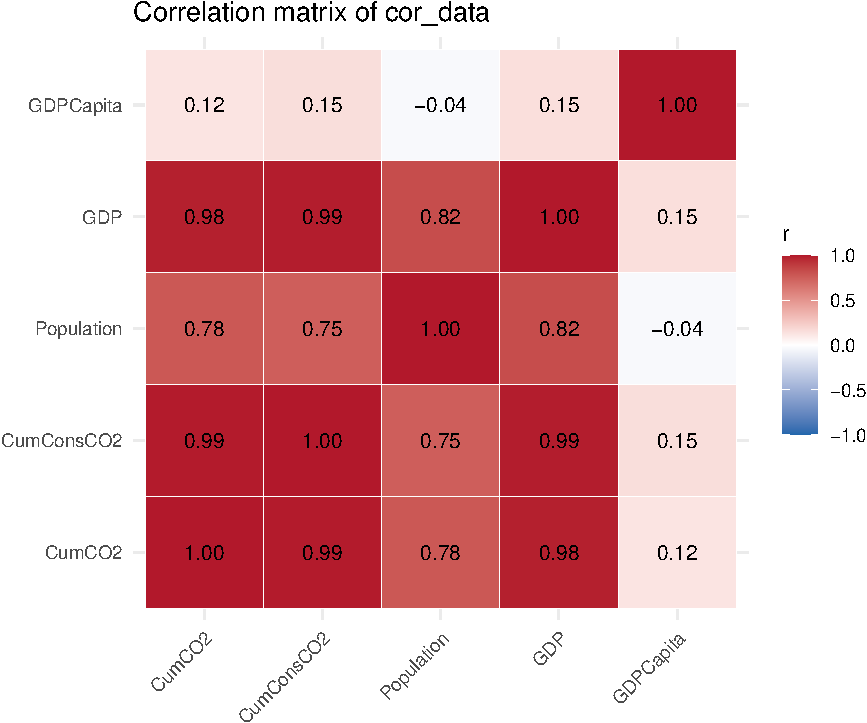
\includegraphics[keepaspectratio]{u3284342_final_assessment_files/figure-latex/t3q2-1.pdf}}

\begin{Shaded}
\begin{Highlighting}[]
\NormalTok{cor\_gdp }\OtherTok{\textless{}{-}} \FunctionTok{cor}\NormalTok{(cor\_data}\SpecialCharTok{$}\NormalTok{CumCO2, cor\_data}\SpecialCharTok{$}\NormalTok{GDP)}
\NormalTok{cor\_gdp\_pc }\OtherTok{\textless{}{-}} \FunctionTok{cor}\NormalTok{(cor\_data}\SpecialCharTok{$}\NormalTok{CumCO2, cor\_data}\SpecialCharTok{$}\NormalTok{GDPCapita)}
\FunctionTok{cat}\NormalTok{(}\StringTok{"cor(CumCO2, GDP)       ="}\NormalTok{, }\FunctionTok{round}\NormalTok{(cor\_gdp, }\DecValTok{2}\NormalTok{), }\StringTok{"}\SpecialCharTok{\textbackslash{}n}\StringTok{"}\NormalTok{)}
\end{Highlighting}
\end{Shaded}

\begin{verbatim}
## cor(CumCO2, GDP)       = 0.98
\end{verbatim}

\begin{Shaded}
\begin{Highlighting}[]
\FunctionTok{cat}\NormalTok{(}\StringTok{"cor(CumCO2, GDPCapita) ="}\NormalTok{, }\FunctionTok{round}\NormalTok{(cor\_gdp\_pc, }\DecValTok{2}\NormalTok{), }\StringTok{"}\SpecialCharTok{\textbackslash{}n}\StringTok{"}\NormalTok{)}
\end{Highlighting}
\end{Shaded}

\begin{verbatim}
## cor(CumCO2, GDPCapita) = 0.12
\end{verbatim}

\emph{Report \texttt{cor(CumCO2,\ GDP)} and
\texttt{cor(CumCO2,\ GDPCapita)}. Why are those two numbers so
different?}

\texttt{cor(CumCO2,\ GDP)} is 0.98 and \texttt{cor(CumCO2,\ GDPCapita)}
is 0.12. They differ because GDP and cumulative emissions are both
measures of \emph{size}: they grow with a country's population and total
economic activity, so the same few giants (China, the United States,
India) top both. GDP per capita removes size and measures wealth per
person, which on its own says little about total emissions: rich but
small countries such as Luxembourg and Singapore have small totals,
while populous middle-income countries such as China (GDP per capita
18,921) and India (7,350) have the largest.

\subsubsection{\texorpdfstring{3.3 Distribution of \texttt{CumCO2}, with
and without
log}{3.3 Distribution of CumCO2, with and without log}}\label{distribution-of-cumco2-with-and-without-log}

\begin{Shaded}
\begin{Highlighting}[]
\FunctionTok{ggplot}\NormalTok{(cor\_data, }\FunctionTok{aes}\NormalTok{(CumCO2)) }\SpecialCharTok{+}
  \FunctionTok{geom\_histogram}\NormalTok{(}\AttributeTok{bins =} \DecValTok{20}\NormalTok{, }\AttributeTok{fill =} \StringTok{"grey60"}\NormalTok{, }\AttributeTok{colour =} \StringTok{"white"}\NormalTok{) }\SpecialCharTok{+}
  \FunctionTok{scale\_x\_continuous}\NormalTok{(}\AttributeTok{labels =} \FunctionTok{label\_comma}\NormalTok{()) }\SpecialCharTok{+}
  \FunctionTok{labs}\NormalTok{(}\AttributeTok{title =} \StringTok{"CumCO2: raw scale"}\NormalTok{, }\AttributeTok{x =} \StringTok{"Cumulative CO2 (Mt)"}\NormalTok{,}
       \AttributeTok{y =} \StringTok{"Number of countries"}\NormalTok{)}
\end{Highlighting}
\end{Shaded}

\pandocbounded{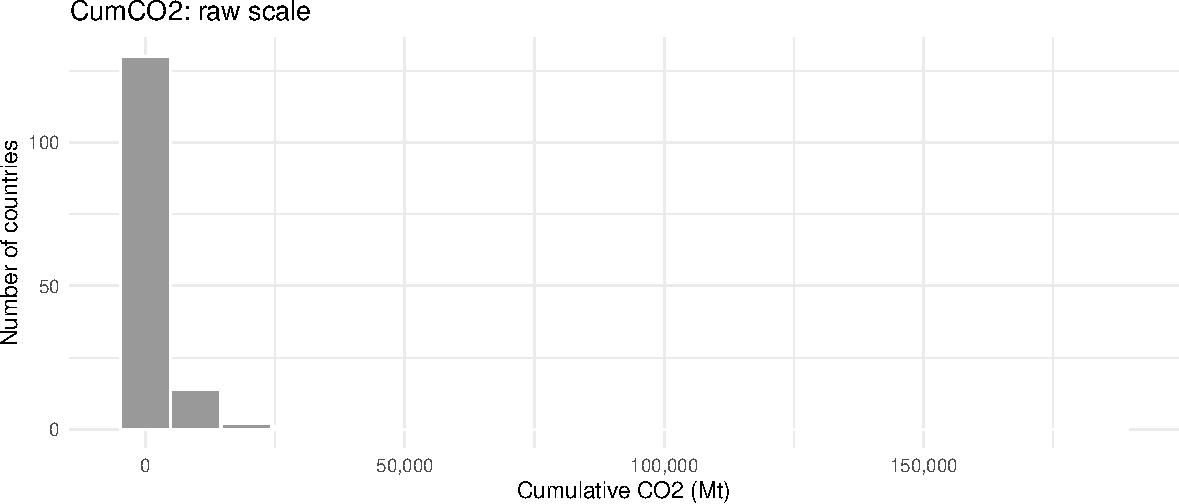
\includegraphics[keepaspectratio]{u3284342_final_assessment_files/figure-latex/t3q3-1.pdf}}

\begin{Shaded}
\begin{Highlighting}[]
\FunctionTok{ggplot}\NormalTok{(}\FunctionTok{filter}\NormalTok{(cor\_data, CumCO2 }\SpecialCharTok{\textgreater{}} \DecValTok{0}\NormalTok{), }\FunctionTok{aes}\NormalTok{(CumCO2)) }\SpecialCharTok{+}
  \FunctionTok{geom\_histogram}\NormalTok{(}\AttributeTok{bins =} \DecValTok{20}\NormalTok{, }\AttributeTok{fill =} \StringTok{"steelblue"}\NormalTok{, }\AttributeTok{colour =} \StringTok{"white"}\NormalTok{) }\SpecialCharTok{+}
  \FunctionTok{scale\_x\_log10}\NormalTok{(}\AttributeTok{labels =} \FunctionTok{label\_comma}\NormalTok{()) }\SpecialCharTok{+}
  \FunctionTok{labs}\NormalTok{(}\AttributeTok{title =} \StringTok{"CumCO2: log10 scale"}\NormalTok{, }\AttributeTok{x =} \StringTok{"Cumulative CO2 (Mt, log scale)"}\NormalTok{,}
       \AttributeTok{y =} \StringTok{"Number of countries"}\NormalTok{)}
\end{Highlighting}
\end{Shaded}

\pandocbounded{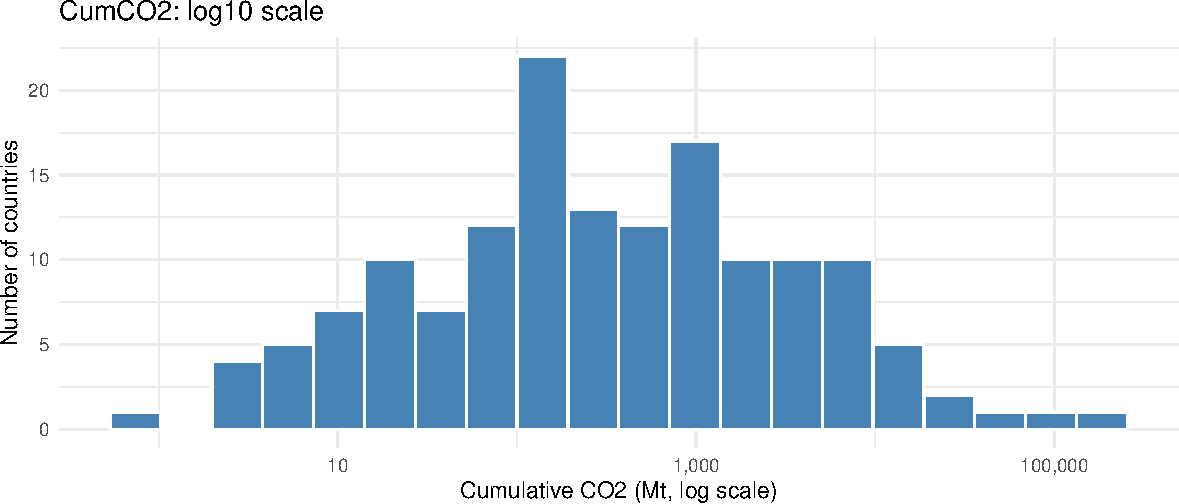
\includegraphics[keepaspectratio]{u3284342_final_assessment_files/figure-latex/t3q3-2.pdf}}

\subsubsection{3.4 Train/test split}\label{traintest-split}

\begin{Shaded}
\begin{Highlighting}[]
\DocumentationTok{\#\# Required — do not remove or change this line:}
\FunctionTok{set.seed}\NormalTok{(}\FunctionTok{seed\_from\_id}\NormalTok{(params}\SpecialCharTok{$}\NormalTok{studentID))}

\CommentTok{\# Your 65/35 split goes below.}
\NormalTok{train\_idx }\OtherTok{\textless{}{-}} \FunctionTok{sample}\NormalTok{(}\FunctionTok{seq\_len}\NormalTok{(}\FunctionTok{nrow}\NormalTok{(cor\_data)),}
                    \AttributeTok{size =} \FunctionTok{round}\NormalTok{(}\FloatTok{0.65} \SpecialCharTok{*} \FunctionTok{nrow}\NormalTok{(cor\_data)))}
\NormalTok{train\_data }\OtherTok{\textless{}{-}}\NormalTok{ cor\_data[train\_idx, ]}
\NormalTok{test\_data }\OtherTok{\textless{}{-}}\NormalTok{ cor\_data[}\SpecialCharTok{{-}}\NormalTok{train\_idx, ]}

\FunctionTok{cat}\NormalTok{(}\StringTok{"Training rows:"}\NormalTok{, }\FunctionTok{nrow}\NormalTok{(train\_data), }\StringTok{"| Testing rows:"}\NormalTok{, }\FunctionTok{nrow}\NormalTok{(test\_data),}
    \StringTok{"}\SpecialCharTok{\textbackslash{}n}\StringTok{"}\NormalTok{)}
\end{Highlighting}
\end{Shaded}

\begin{verbatim}
## Training rows: 98 | Testing rows: 52
\end{verbatim}

\subsubsection{\texorpdfstring{3.5 Linear model:
\texttt{CumCO2\ \textasciitilde{}\ GDP}}{3.5 Linear model: CumCO2 \textasciitilde{} GDP}}\label{linear-model-cumco2-gdp}

\begin{Shaded}
\begin{Highlighting}[]
\NormalTok{model\_gdp }\OtherTok{\textless{}{-}} \FunctionTok{lm}\NormalTok{(CumCO2 }\SpecialCharTok{\textasciitilde{}}\NormalTok{ GDP, }\AttributeTok{data =}\NormalTok{ train\_data)}
\FunctionTok{summary}\NormalTok{(model\_gdp)}
\end{Highlighting}
\end{Shaded}

\begin{verbatim}
## 
## Call:
## lm(formula = CumCO2 ~ GDP, data = train_data)
## 
## Residuals:
##      Min       1Q   Median       3Q      Max 
## -22815.8   -190.2    740.0    884.3  19212.1 
## 
## Coefficients:
##               Estimate Std. Error t value Pr(>|t|)    
## (Intercept) -8.905e+02  4.274e+02  -2.083   0.0399 *  
## GDP          6.162e-03  1.175e-04  52.450   <2e-16 ***
## ---
## Signif. codes:  0 '***' 0.001 '**' 0.01 '*' 0.05 '.' 0.1 ' ' 1
## 
## Residual standard error: 4066 on 96 degrees of freedom
## Multiple R-squared:  0.9663, Adjusted R-squared:  0.9659 
## F-statistic:  2751 on 1 and 96 DF,  p-value: < 2.2e-16
\end{verbatim}

\begin{Shaded}
\begin{Highlighting}[]
\NormalTok{pred\_gdp }\OtherTok{\textless{}{-}} \FunctionTok{predict}\NormalTok{(model\_gdp, }\AttributeTok{newdata =}\NormalTok{ test\_data)}
\NormalTok{rmse\_gdp }\OtherTok{\textless{}{-}} \FunctionTok{Rmse}\NormalTok{(test\_data}\SpecialCharTok{$}\NormalTok{CumCO2, pred\_gdp)}
\NormalTok{r2\_gdp }\OtherTok{\textless{}{-}} \FunctionTok{RSquared}\NormalTok{(test\_data}\SpecialCharTok{$}\NormalTok{CumCO2, pred\_gdp)}
\FunctionTok{cat}\NormalTok{(}\StringTok{"Test RMSE (GDP only):"}\NormalTok{, }\FunctionTok{round}\NormalTok{(rmse\_gdp, }\DecValTok{2}\NormalTok{), }\StringTok{"Mt | Test R2:"}\NormalTok{,}
    \FunctionTok{round}\NormalTok{(r2\_gdp, }\DecValTok{3}\NormalTok{), }\StringTok{"}\SpecialCharTok{\textbackslash{}n}\StringTok{"}\NormalTok{)}
\end{Highlighting}
\end{Shaded}

\begin{verbatim}
## Test RMSE (GDP only): 1719.84 Mt | Test R2: 0.812
\end{verbatim}

\subsubsection{3.6 Linear model: all
predictors}\label{linear-model-all-predictors}

\begin{Shaded}
\begin{Highlighting}[]
\NormalTok{model\_full }\OtherTok{\textless{}{-}} \FunctionTok{lm}\NormalTok{(CumCO2 }\SpecialCharTok{\textasciitilde{}}\NormalTok{ CumConsCO2 }\SpecialCharTok{+}\NormalTok{ Population }\SpecialCharTok{+}\NormalTok{ GDP }\SpecialCharTok{+}\NormalTok{ GDPCapita,}
                 \AttributeTok{data =}\NormalTok{ train\_data)}
\FunctionTok{summary}\NormalTok{(model\_full)}
\end{Highlighting}
\end{Shaded}

\begin{verbatim}
## 
## Call:
## lm(formula = CumCO2 ~ CumConsCO2 + Population + GDP + GDPCapita, 
##     data = train_data)
## 
## Residuals:
##     Min      1Q  Median      3Q     Max 
## -5759.4  -240.8    53.0   215.3  4223.3 
## 
## Coefficients:
##               Estimate Std. Error t value Pr(>|t|)    
## (Intercept) -2.542e+02  1.829e+02  -1.390    0.168    
## CumConsCO2   1.786e+00  6.470e-02  27.605   <2e-16 ***
## Population   2.479e-05  1.772e-06  13.991   <2e-16 ***
## GDP         -5.204e-03  4.401e-04 -11.826   <2e-16 ***
## GDPCapita    5.963e-03  6.247e-03   0.955    0.342    
## ---
## Signif. codes:  0 '***' 0.001 '**' 0.01 '*' 0.05 '.' 0.1 ' ' 1
## 
## Residual standard error: 1270 on 93 degrees of freedom
## Multiple R-squared:  0.9968, Adjusted R-squared:  0.9967 
## F-statistic:  7277 on 4 and 93 DF,  p-value: < 2.2e-16
\end{verbatim}

\begin{Shaded}
\begin{Highlighting}[]
\NormalTok{pred\_full }\OtherTok{\textless{}{-}} \FunctionTok{predict}\NormalTok{(model\_full, }\AttributeTok{newdata =}\NormalTok{ test\_data)}
\NormalTok{rmse\_full }\OtherTok{\textless{}{-}} \FunctionTok{Rmse}\NormalTok{(test\_data}\SpecialCharTok{$}\NormalTok{CumCO2, pred\_full)}
\NormalTok{r2\_full }\OtherTok{\textless{}{-}} \FunctionTok{RSquared}\NormalTok{(test\_data}\SpecialCharTok{$}\NormalTok{CumCO2, pred\_full)}
\FunctionTok{cat}\NormalTok{(}\StringTok{"Test RMSE (all predictors):"}\NormalTok{, }\FunctionTok{round}\NormalTok{(rmse\_full, }\DecValTok{2}\NormalTok{), }\StringTok{"Mt | Test R2:"}\NormalTok{,}
    \FunctionTok{round}\NormalTok{(r2\_full, }\DecValTok{3}\NormalTok{), }\StringTok{"}\SpecialCharTok{\textbackslash{}n}\StringTok{"}\NormalTok{)}
\end{Highlighting}
\end{Shaded}

\begin{verbatim}
## Test RMSE (all predictors): 647.46 Mt | Test R2: 0.973
\end{verbatim}

\subsubsection{3.7 Interpret and compare the two
models}\label{interpret-and-compare-the-two-models}

\emph{When should the first be preferred, and when the second? If the
full model has the higher test RMSE, explain why --- that is not an
error.}

On the 52 test countries, the full model clearly outperforms the
GDP-only model: its test RMSE is 647.46 Mt against 1,719.84 Mt, and its
test R² is 0.973 against 0.812. In my split, the model with more
predictors therefore does \emph{not} have the higher test RMSE. Its
advantage comes almost entirely from \texttt{CumConsCO2}, which
correlates 0.99 with \texttt{CumCO2}. This is close to target leakage:
consumption-based emissions are production-based emissions adjusted for
trade, and for the 55 countries without consumption data
\texttt{CumConsCO2} was set equal to \texttt{CumCO2} in Task 1.6, so the
model partly learns an identity.

The GDP-only model should be preferred when the aim is explanation or
when consumption data are unavailable. It is easy to interpret: each
additional million dollars of GDP is associated with 0.00616 Mt (about
6,200 t) more cumulative CO2 since 2004. Its single coefficient is also
stable, whereas the full model's coefficients are distorted by
multicollinearity: GDP receives a \emph{negative} coefficient (-0.0052
Mt per million dollars) and GDPCapita is not significant (p = 0.342),
because GDP and \texttt{CumConsCO2} carry almost the same information (r
= 0.99).

The full model is better for pure prediction when every predictor,
including genuine consumption-based data, is available for the country
being predicted.

Had the full model's test RMSE been higher, that would not have been an
error: extra correlated predictors can overfit the 98 training countries
and generalise worse, and with only 52 test countries a single large
emitter can swing the RMSE.

\subsubsection{3.8 Alternative models}\label{alternative-models}

\begin{Shaded}
\begin{Highlighting}[]
\NormalTok{predictors }\OtherTok{\textless{}{-}} \FunctionTok{c}\NormalTok{(}\StringTok{"CumConsCO2"}\NormalTok{, }\StringTok{"Population"}\NormalTok{, }\StringTok{"GDP"}\NormalTok{, }\StringTok{"GDPCapita"}\NormalTok{)}
\NormalTok{x\_train }\OtherTok{\textless{}{-}} \FunctionTok{as.matrix}\NormalTok{(train\_data[, predictors])}
\NormalTok{x\_test }\OtherTok{\textless{}{-}} \FunctionTok{as.matrix}\NormalTok{(test\_data[, predictors])}
\NormalTok{y\_train }\OtherTok{\textless{}{-}}\NormalTok{ train\_data}\SpecialCharTok{$}\NormalTok{CumCO2}
\NormalTok{y\_test }\OtherTok{\textless{}{-}}\NormalTok{ test\_data}\SpecialCharTok{$}\NormalTok{CumCO2}

\CommentTok{\# Cross{-}validation folds are random; seeding again makes the lambda}
\CommentTok{\# choice reproducible. The train/test split above is unaffected.}
\FunctionTok{set.seed}\NormalTok{(}\FunctionTok{seed\_from\_id}\NormalTok{(params}\SpecialCharTok{$}\NormalTok{studentID))}

\CommentTok{\# Ridge (alpha = 0) and lasso (alpha = 1); lambda chosen by 5{-}fold CV}
\CommentTok{\# (5 rather than 10 folds because the training set is small).}
\NormalTok{ridge\_cv }\OtherTok{\textless{}{-}} \FunctionTok{cv.glmnet}\NormalTok{(x\_train, y\_train, }\AttributeTok{alpha =} \DecValTok{0}\NormalTok{, }\AttributeTok{nfolds =} \DecValTok{5}\NormalTok{)}
\NormalTok{lasso\_cv }\OtherTok{\textless{}{-}} \FunctionTok{cv.glmnet}\NormalTok{(x\_train, y\_train, }\AttributeTok{alpha =} \DecValTok{1}\NormalTok{, }\AttributeTok{nfolds =} \DecValTok{5}\NormalTok{)}
\NormalTok{pred\_ridge }\OtherTok{\textless{}{-}} \FunctionTok{as.numeric}\NormalTok{(}\FunctionTok{predict}\NormalTok{(ridge\_cv, }\AttributeTok{newx =}\NormalTok{ x\_test,}
                                 \AttributeTok{s =} \StringTok{"lambda.min"}\NormalTok{))}
\NormalTok{pred\_lasso }\OtherTok{\textless{}{-}} \FunctionTok{as.numeric}\NormalTok{(}\FunctionTok{predict}\NormalTok{(lasso\_cv, }\AttributeTok{newx =}\NormalTok{ x\_test,}
                                 \AttributeTok{s =} \StringTok{"lambda.min"}\NormalTok{))}
\FunctionTok{coef}\NormalTok{(lasso\_cv, }\AttributeTok{s =} \StringTok{"lambda.min"}\NormalTok{)  }\CommentTok{\# which predictors lasso keeps}
\end{Highlighting}
\end{Shaded}

\begin{verbatim}
## 5 x 1 sparse Matrix of class "dgCMatrix"
##                lambda.min
## (Intercept) -1.926611e+02
## CumConsCO2   1.025043e+00
## Population   7.130379e-06
## GDP          .           
## GDPCapita   -9.325435e-03
\end{verbatim}

\begin{Shaded}
\begin{Highlighting}[]
\CommentTok{\# Regression tree, pruned at the complexity with lowest CV error.}
\NormalTok{tree\_fit }\OtherTok{\textless{}{-}} \FunctionTok{rpart}\NormalTok{(CumCO2 }\SpecialCharTok{\textasciitilde{}}\NormalTok{ ., }\AttributeTok{data =}\NormalTok{ train\_data, }\AttributeTok{method =} \StringTok{"anova"}\NormalTok{,}
                  \AttributeTok{control =} \FunctionTok{rpart.control}\NormalTok{(}\AttributeTok{minsplit =} \DecValTok{6}\NormalTok{, }\AttributeTok{cp =} \FloatTok{0.001}\NormalTok{))}
\NormalTok{best\_cp }\OtherTok{\textless{}{-}}\NormalTok{ tree\_fit}\SpecialCharTok{$}\NormalTok{cptable[}\FunctionTok{which.min}\NormalTok{(tree\_fit}\SpecialCharTok{$}\NormalTok{cptable[, }\StringTok{"xerror"}\NormalTok{]), }\StringTok{"CP"}\NormalTok{]}
\NormalTok{tree\_pruned }\OtherTok{\textless{}{-}} \FunctionTok{prune}\NormalTok{(tree\_fit, }\AttributeTok{cp =}\NormalTok{ best\_cp)}
\NormalTok{pred\_tree }\OtherTok{\textless{}{-}} \FunctionTok{predict}\NormalTok{(tree\_pruned, }\AttributeTok{newdata =}\NormalTok{ test\_data)}

\CommentTok{\# Log{-}log linear model: addresses the skew seen in 3.3 and 3A.}
\CommentTok{\# log1p() keeps zero values defined; predictions are back{-}transformed.}
\NormalTok{model\_log }\OtherTok{\textless{}{-}} \FunctionTok{lm}\NormalTok{(}\FunctionTok{log1p}\NormalTok{(CumCO2) }\SpecialCharTok{\textasciitilde{}} \FunctionTok{log1p}\NormalTok{(CumConsCO2) }\SpecialCharTok{+} \FunctionTok{log1p}\NormalTok{(Population) }\SpecialCharTok{+}
                  \FunctionTok{log1p}\NormalTok{(GDP) }\SpecialCharTok{+} \FunctionTok{log1p}\NormalTok{(GDPCapita), }\AttributeTok{data =}\NormalTok{ train\_data)}
\NormalTok{pred\_log }\OtherTok{\textless{}{-}} \FunctionTok{expm1}\NormalTok{(}\FunctionTok{predict}\NormalTok{(model\_log, }\AttributeTok{newdata =}\NormalTok{ test\_data))}

\NormalTok{model\_comparison }\OtherTok{\textless{}{-}} \FunctionTok{tibble}\NormalTok{(}
  \AttributeTok{Model =} \FunctionTok{c}\NormalTok{(}\StringTok{"Linear (GDP only)"}\NormalTok{, }\StringTok{"Linear (all variables)"}\NormalTok{,}
            \StringTok{"Ridge (all variables)"}\NormalTok{, }\StringTok{"Lasso (all variables)"}\NormalTok{,}
            \StringTok{"Regression tree"}\NormalTok{, }\StringTok{"Log{-}log linear (all variables)"}\NormalTok{),}
  \AttributeTok{RMSE =} \FunctionTok{c}\NormalTok{(rmse\_gdp, rmse\_full, }\FunctionTok{Rmse}\NormalTok{(y\_test, pred\_ridge),}
           \FunctionTok{Rmse}\NormalTok{(y\_test, pred\_lasso), }\FunctionTok{Rmse}\NormalTok{(y\_test, pred\_tree),}
           \FunctionTok{Rmse}\NormalTok{(y\_test, pred\_log)),}
  \AttributeTok{R\_squared =} \FunctionTok{c}\NormalTok{(r2\_gdp, r2\_full, }\FunctionTok{RSquared}\NormalTok{(y\_test, pred\_ridge),}
                \FunctionTok{RSquared}\NormalTok{(y\_test, pred\_lasso), }\FunctionTok{RSquared}\NormalTok{(y\_test, pred\_tree),}
                \FunctionTok{RSquared}\NormalTok{(y\_test, pred\_log))}
\NormalTok{) }\SpecialCharTok{\%\textgreater{}\%}
  \FunctionTok{arrange}\NormalTok{(RMSE)}

\FunctionTok{kable}\NormalTok{(model\_comparison, }\AttributeTok{digits =} \DecValTok{3}\NormalTok{, }\AttributeTok{format.args =} \FunctionTok{list}\NormalTok{(}\AttributeTok{big.mark =} \StringTok{","}\NormalTok{),}
      \AttributeTok{caption =} \StringTok{"Test{-}set performance (RMSE in Mt CO2)"}\NormalTok{)}
\end{Highlighting}
\end{Shaded}

\begin{longtable}[]{@{}lrr@{}}
\caption{Test-set performance (RMSE in Mt CO2)}\tabularnewline
\toprule\noalign{}
Model & RMSE & R\_squared \\
\midrule\noalign{}
\endfirsthead
\toprule\noalign{}
Model & RMSE & R\_squared \\
\midrule\noalign{}
\endhead
\bottomrule\noalign{}
\endlastfoot
Log-log linear (all variables) & 577.657 & 0.979 \\
Linear (all variables) & 647.459 & 0.973 \\
Lasso (all variables) & 985.146 & 0.938 \\
Ridge (all variables) & 1,089.573 & 0.924 \\
Linear (GDP only) & 1,719.835 & 0.812 \\
Regression tree & 2,075.521 & 0.726 \\
\end{longtable}

The log-log linear model performs best (test RMSE 577.66 Mt, R² 0.979),
because modelling every variable on a log scale removes the extreme
right skew of \texttt{CumCO2} (3.3) so that a few giants no longer
dominate the fit. The plain full linear model is second (647.46 Mt).
Regularisation did not help: lasso (985.15 Mt) and ridge (1,089.57 Mt)
shrink coefficients towards zero, which costs accuracy when there are
only four predictors and a strong signal. Lasso's coefficients are
informative, though: it dropped GDP entirely and kept
\texttt{CumConsCO2} (coefficient 1.03), confirming that GDP adds nothing
once consumption emissions are known. The regression tree is worst
(2,075.52 Mt, R² 0.726): its predictions are piecewise constant, and
with only a handful of very large countries in 98 training rows it
cannot represent the extreme values that dominate RMSE.

\begin{center}\rule{0.5\linewidth}{0.5pt}\end{center}

\subsection{3A. Assumption checking}\label{a.-assumption-checking}

\subsubsection{i. Linearity}\label{i.-linearity}

\begin{Shaded}
\begin{Highlighting}[]
\NormalTok{train\_long }\OtherTok{\textless{}{-}}\NormalTok{ train\_data }\SpecialCharTok{\%\textgreater{}\%}
  \FunctionTok{rownames\_to\_column}\NormalTok{(}\StringTok{"Country"}\NormalTok{) }\SpecialCharTok{\%\textgreater{}\%}
  \FunctionTok{pivot\_longer}\NormalTok{(}\FunctionTok{all\_of}\NormalTok{(predictors), }\AttributeTok{names\_to =} \StringTok{"Predictor"}\NormalTok{,}
               \AttributeTok{values\_to =} \StringTok{"Value"}\NormalTok{)}

\CommentTok{\# Solid line: linear fit. Dashed line: flexible (loess) fit. Where the two}
\CommentTok{\# diverge, a straight line is a poor description of the relationship.}
\FunctionTok{ggplot}\NormalTok{(train\_long, }\FunctionTok{aes}\NormalTok{(Value, CumCO2)) }\SpecialCharTok{+}
  \FunctionTok{geom\_point}\NormalTok{(}\AttributeTok{alpha =} \FloatTok{0.7}\NormalTok{) }\SpecialCharTok{+}
  \FunctionTok{geom\_smooth}\NormalTok{(}\AttributeTok{method =} \StringTok{"lm"}\NormalTok{, }\AttributeTok{se =} \ConstantTok{FALSE}\NormalTok{, }\AttributeTok{colour =} \StringTok{"steelblue"}\NormalTok{) }\SpecialCharTok{+}
  \FunctionTok{geom\_smooth}\NormalTok{(}\AttributeTok{method =} \StringTok{"loess"}\NormalTok{, }\AttributeTok{se =} \ConstantTok{FALSE}\NormalTok{, }\AttributeTok{span =} \FloatTok{0.9}\NormalTok{,}
              \AttributeTok{colour =} \StringTok{"firebrick"}\NormalTok{, }\AttributeTok{linetype =} \StringTok{"dashed"}\NormalTok{) }\SpecialCharTok{+}
  \FunctionTok{facet\_wrap}\NormalTok{(}\SpecialCharTok{\textasciitilde{}}\NormalTok{ Predictor, }\AttributeTok{scales =} \StringTok{"free\_x"}\NormalTok{) }\SpecialCharTok{+}
  \FunctionTok{scale\_x\_continuous}\NormalTok{(}\AttributeTok{labels =} \FunctionTok{label\_comma}\NormalTok{()) }\SpecialCharTok{+}
  \FunctionTok{scale\_y\_continuous}\NormalTok{(}\AttributeTok{labels =} \FunctionTok{label\_comma}\NormalTok{()) }\SpecialCharTok{+}
  \FunctionTok{labs}\NormalTok{(}\AttributeTok{title =} \StringTok{"CumCO2 against each predictor (training data)"}\NormalTok{,}
       \AttributeTok{x =} \StringTok{"Predictor value"}\NormalTok{, }\AttributeTok{y =} \StringTok{"Cumulative CO2 (Mt)"}\NormalTok{)}
\end{Highlighting}
\end{Shaded}

\pandocbounded{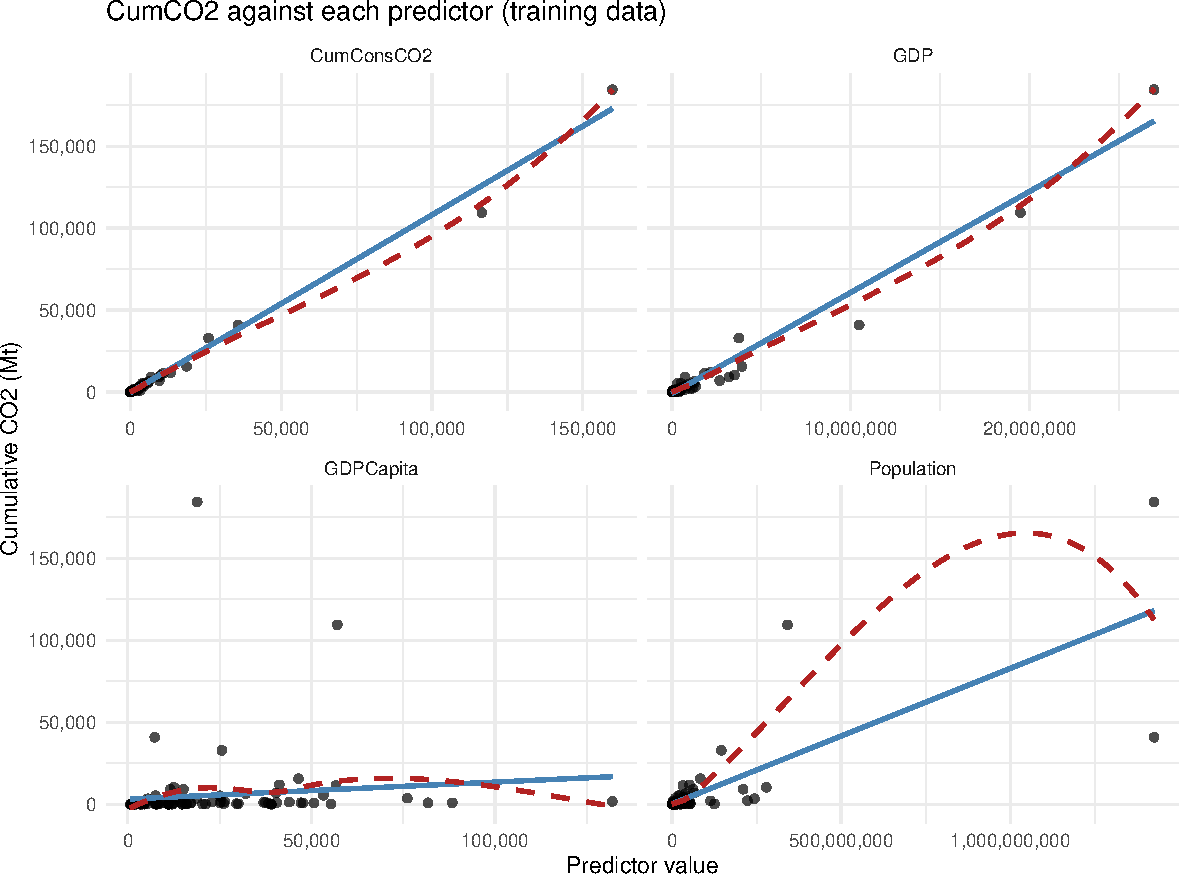
\includegraphics[keepaspectratio]{u3284342_final_assessment_files/figure-latex/t3a-linearity-1.pdf}}

\begin{Shaded}
\begin{Highlighting}[]
\CommentTok{\# Pearson measures linear association, Spearman monotonic association; a}
\CommentTok{\# large gap between them signals a non{-}linear relationship.}
\NormalTok{train\_long }\SpecialCharTok{\%\textgreater{}\%}
  \FunctionTok{group\_by}\NormalTok{(Predictor) }\SpecialCharTok{\%\textgreater{}\%}
  \FunctionTok{summarise}\NormalTok{(}\AttributeTok{Pearson =} \FunctionTok{cor}\NormalTok{(Value, CumCO2),}
            \AttributeTok{Spearman =} \FunctionTok{cor}\NormalTok{(Value, CumCO2, }\AttributeTok{method =} \StringTok{"spearman"}\NormalTok{),}
            \AttributeTok{Gap =}\NormalTok{ Spearman }\SpecialCharTok{{-}}\NormalTok{ Pearson, }\AttributeTok{.groups =} \StringTok{"drop"}\NormalTok{) }\SpecialCharTok{\%\textgreater{}\%}
  \FunctionTok{kable}\NormalTok{(}\AttributeTok{digits =} \DecValTok{3}\NormalTok{)}
\end{Highlighting}
\end{Shaded}

{\def\LTcaptype{none} % do not increment counter
\begin{longtable}[]{@{}lrrr@{}}
\toprule\noalign{}
Predictor & Pearson & Spearman & Gap \\
\midrule\noalign{}
\endhead
\bottomrule\noalign{}
\endlastfoot
CumConsCO2 & 0.995 & 0.988 & -0.007 \\
GDP & 0.983 & 0.947 & -0.036 \\
GDPCapita & 0.105 & 0.533 & 0.429 \\
Population & 0.776 & 0.687 & -0.089 \\
\end{longtable}
}

\emph{Does a linear relationship look reasonable? Which predictor
departs from it most clearly?}

A linear relationship looks reasonable for \texttt{CumConsCO2} and
\texttt{GDP}: the linear and loess fits nearly coincide, and the Pearson
correlations (0.995 and 0.983) match the Spearman rank correlations
(0.988 and 0.947). This fit is largely driven by a few very large
countries, though, with most countries bunched near the origin.
\texttt{GDPCapita} departs from linearity most clearly: its linear
correlation is only 0.105, but its rank correlation is 0.533, a gap of
0.429, so richer countries do tend to emit more but not in a straight
line. \texttt{Population} also curves visibly, because China and India
have similar populations but very different emissions.

\subsubsection{ii. Distribution of the
response}\label{ii.-distribution-of-the-response}

\begin{Shaded}
\begin{Highlighting}[]
\CommentTok{\# Numerical support for the 3.3 histograms: a strongly right{-}skewed}
\CommentTok{\# variable has a mean far above its median.}
\FunctionTok{c}\NormalTok{(}\AttributeTok{Mean =} \FunctionTok{mean}\NormalTok{(train\_data}\SpecialCharTok{$}\NormalTok{CumCO2), }\AttributeTok{Median =} \FunctionTok{median}\NormalTok{(train\_data}\SpecialCharTok{$}\NormalTok{CumCO2))}
\end{Highlighting}
\end{Shaded}

\begin{verbatim}
##      Mean    Median 
## 5312.5320  362.1947
\end{verbatim}

\begin{Shaded}
\begin{Highlighting}[]
\FunctionTok{shapiro.test}\NormalTok{(train\_data}\SpecialCharTok{$}\NormalTok{CumCO2)}
\end{Highlighting}
\end{Shaded}

\begin{verbatim}
## 
##  Shapiro-Wilk normality test
## 
## data:  train_data$CumCO2
## W = 0.23617, p-value < 2.2e-16
\end{verbatim}

\begin{Shaded}
\begin{Highlighting}[]
\FunctionTok{shapiro.test}\NormalTok{(}\FunctionTok{log1p}\NormalTok{(train\_data}\SpecialCharTok{$}\NormalTok{CumCO2))}
\end{Highlighting}
\end{Shaded}

\begin{verbatim}
## 
##  Shapiro-Wilk normality test
## 
## data:  log1p(train_data$CumCO2)
## W = 0.99406, p-value = 0.9471
\end{verbatim}

\emph{Using your plots from 3.3 --- does raw \texttt{CumCO2} satisfy the
normality assumption? Is a transformation warranted?}

No.~The raw histogram in 3.3 puts almost every country in the first bin,
with a long right tail out to China (184,474.9 Mt). In the training data
the mean (5,312.5 Mt) is almost 15 times the median (362.2 Mt), and the
Shapiro--Wilk test rejects normality decisively (W = 0.236, p
\textless{} 2.2e-16). On the log scale the histogram is roughly
symmetric and the test no longer rejects normality (W = 0.994, p =
0.947), so a log transformation is warranted. Strictly, the assumption
applies to the residuals rather than the response, but a response this
skewed produces skewed residuals, as the Q--Q plot in iii confirms.

\subsubsection{iii. Residual
diagnostics}\label{iii.-residual-diagnostics}

\begin{Shaded}
\begin{Highlighting}[]
\FunctionTok{par}\NormalTok{(}\AttributeTok{mfrow =} \FunctionTok{c}\NormalTok{(}\DecValTok{2}\NormalTok{, }\DecValTok{2}\NormalTok{))}
\FunctionTok{plot}\NormalTok{(model\_full, }\AttributeTok{which =} \FunctionTok{c}\NormalTok{(}\DecValTok{1}\NormalTok{, }\DecValTok{2}\NormalTok{, }\DecValTok{3}\NormalTok{, }\DecValTok{5}\NormalTok{))}
\end{Highlighting}
\end{Shaded}

\pandocbounded{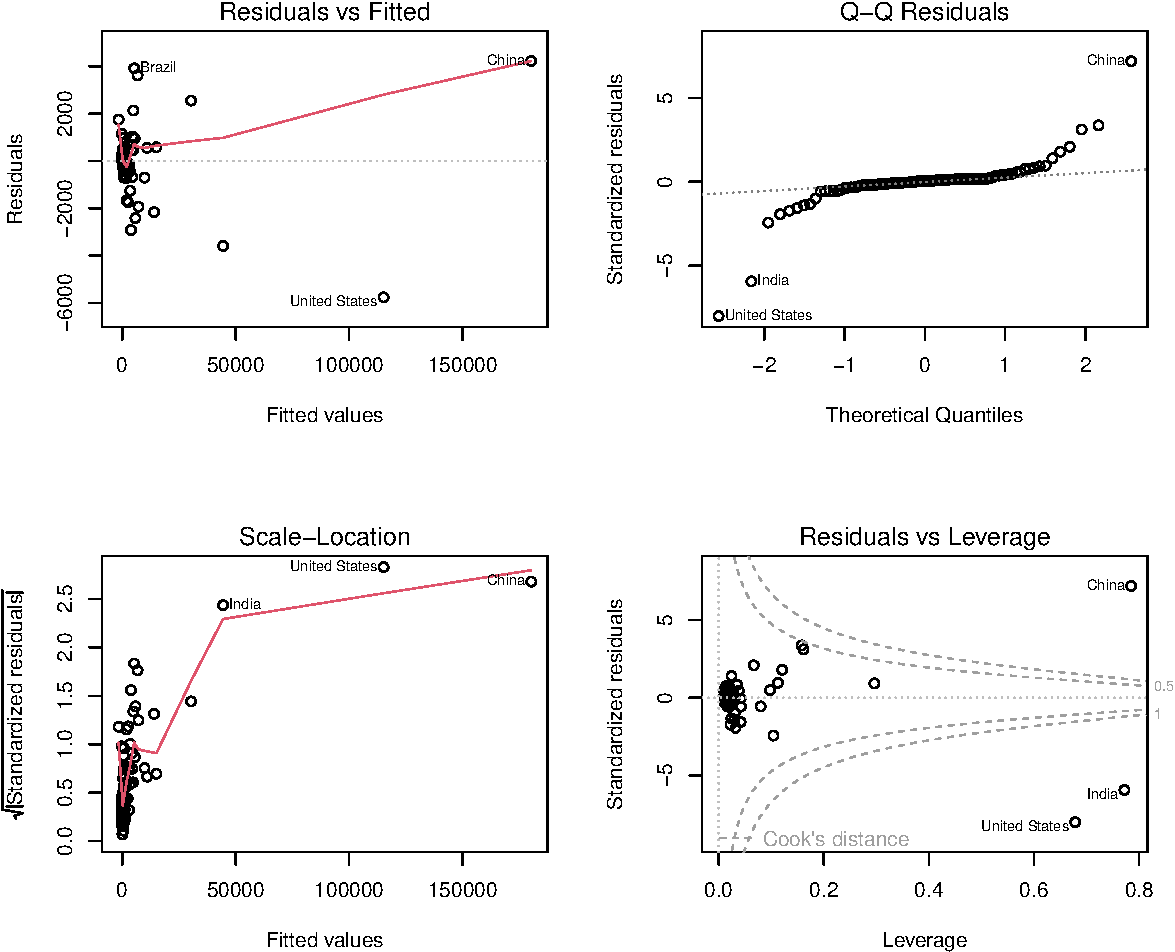
\includegraphics[keepaspectratio]{u3284342_final_assessment_files/figure-latex/t3a-diagnostics-1.pdf}}

\begin{Shaded}
\begin{Highlighting}[]
\FunctionTok{par}\NormalTok{(}\AttributeTok{mfrow =} \FunctionTok{c}\NormalTok{(}\DecValTok{1}\NormalTok{, }\DecValTok{1}\NormalTok{))}
\end{Highlighting}
\end{Shaded}

{\def\LTcaptype{none} % do not increment counter
\begin{longtable}[]{@{}
  >{\raggedright\arraybackslash}p{(\linewidth - 4\tabcolsep) * \real{0.3014}}
  >{\raggedright\arraybackslash}p{(\linewidth - 4\tabcolsep) * \real{0.3288}}
  >{\raggedright\arraybackslash}p{(\linewidth - 4\tabcolsep) * \real{0.3699}}@{}}
\toprule\noalign{}
\begin{minipage}[b]{\linewidth}\raggedright
Plot
\end{minipage} & \begin{minipage}[b]{\linewidth}\raggedright
What assumption it tests
\end{minipage} & \begin{minipage}[b]{\linewidth}\raggedright
Does your model satisfy it?
\end{minipage} \\
\midrule\noalign{}
\endhead
\bottomrule\noalign{}
\endlastfoot
Residuals vs Fitted & Linearity: residuals should scatter randomly
around 0 at every fitted value & No: the red line curves upward, with
China's residual far above 0 and the United States' at about -5,800 \\
Normal Q-Q & Normality of the residuals: points should follow the
diagonal & No: both tails leave the line, with China above +5 and India
and the United States below -5 standardised residuals \\
Scale-Location & Constant variance (homoscedasticity): the line should
be flat & No: the line rises steeply from about 0.5 to 2.5, so the error
spread grows with the size of the country \\
Residuals vs Leverage & Influential observations: no point should lie
beyond the Cook's distance contours & No: China (leverage 0.785), India
(0.772) and the United States (0.678) lie beyond the Cook's distance 1
contour, against a threshold of 0.102 \\
\end{longtable}
}

\subsubsection{iv. Influential
observations}\label{iv.-influential-observations}

\begin{Shaded}
\begin{Highlighting}[]
\CommentTok{\# Leverage (hat value) and Cook\textquotesingle{}s distance for each training country.}
\CommentTok{\# Rule of thumb: leverage above 2p/n is high.}
\NormalTok{p }\OtherTok{\textless{}{-}} \FunctionTok{length}\NormalTok{(}\FunctionTok{coef}\NormalTok{(model\_full))}
\NormalTok{n }\OtherTok{\textless{}{-}} \FunctionTok{nrow}\NormalTok{(train\_data)}
\NormalTok{influence\_tbl }\OtherTok{\textless{}{-}} \FunctionTok{tibble}\NormalTok{(}\AttributeTok{Country =} \FunctionTok{names}\NormalTok{(}\FunctionTok{hatvalues}\NormalTok{(model\_full)),}
                        \AttributeTok{Leverage =} \FunctionTok{hatvalues}\NormalTok{(model\_full),}
                        \AttributeTok{CooksD =} \FunctionTok{cooks.distance}\NormalTok{(model\_full)) }\SpecialCharTok{\%\textgreater{}\%}
  \FunctionTok{arrange}\NormalTok{(}\FunctionTok{desc}\NormalTok{(Leverage))}

\FunctionTok{cat}\NormalTok{(}\StringTok{"High{-}leverage threshold (2p/n):"}\NormalTok{, }\FunctionTok{round}\NormalTok{(}\DecValTok{2} \SpecialCharTok{*}\NormalTok{ p }\SpecialCharTok{/}\NormalTok{ n, }\DecValTok{3}\NormalTok{), }\StringTok{"}\SpecialCharTok{\textbackslash{}n}\StringTok{"}\NormalTok{)}
\end{Highlighting}
\end{Shaded}

\begin{verbatim}
## High-leverage threshold (2p/n): 0.102
\end{verbatim}

\begin{Shaded}
\begin{Highlighting}[]
\FunctionTok{kable}\NormalTok{(}\FunctionTok{head}\NormalTok{(influence\_tbl, }\DecValTok{5}\NormalTok{), }\AttributeTok{digits =} \DecValTok{3}\NormalTok{)}
\end{Highlighting}
\end{Shaded}

{\def\LTcaptype{none} % do not increment counter
\begin{longtable}[]{@{}lrr@{}}
\toprule\noalign{}
Country & Leverage & CooksD \\
\midrule\noalign{}
\endhead
\bottomrule\noalign{}
\endlastfoot
China & 0.785 & 37.646 \\
India & 0.772 & 23.846 \\
United States & 0.678 & 27.010 \\
Qatar & 0.296 & 0.071 \\
Indonesia & 0.162 & 0.373 \\
\end{longtable}
}

\begin{Shaded}
\begin{Highlighting}[]
\NormalTok{high\_lev\_country }\OtherTok{\textless{}{-}}\NormalTok{ influence\_tbl}\SpecialCharTok{$}\NormalTok{Country[}\DecValTok{1}\NormalTok{]}
\FunctionTok{cat}\NormalTok{(}\StringTok{"High{-}leverage country:"}\NormalTok{, high\_lev\_country, }\StringTok{"}\SpecialCharTok{\textbackslash{}n}\StringTok{"}\NormalTok{)}
\end{Highlighting}
\end{Shaded}

\begin{verbatim}
## High-leverage country: China
\end{verbatim}

\begin{Shaded}
\begin{Highlighting}[]
\NormalTok{model\_full\_drop }\OtherTok{\textless{}{-}} \FunctionTok{lm}\NormalTok{(CumCO2 }\SpecialCharTok{\textasciitilde{}}\NormalTok{ CumConsCO2 }\SpecialCharTok{+}\NormalTok{ Population }\SpecialCharTok{+}\NormalTok{ GDP }\SpecialCharTok{+}\NormalTok{ GDPCapita,}
                      \AttributeTok{data =}\NormalTok{ train\_data[}\FunctionTok{rownames}\NormalTok{(train\_data) }\SpecialCharTok{!=}
\NormalTok{                                          high\_lev\_country, ])}
\NormalTok{rmse\_full\_drop }\OtherTok{\textless{}{-}} \FunctionTok{Rmse}\NormalTok{(test\_data}\SpecialCharTok{$}\NormalTok{CumCO2,}
                       \FunctionTok{predict}\NormalTok{(model\_full\_drop, }\AttributeTok{newdata =}\NormalTok{ test\_data))}
\FunctionTok{cat}\NormalTok{(}\StringTok{"Test RMSE with"}\NormalTok{, high\_lev\_country, }\StringTok{"removed:"}\NormalTok{,}
    \FunctionTok{round}\NormalTok{(rmse\_full\_drop, }\DecValTok{2}\NormalTok{), }\StringTok{"Mt (was"}\NormalTok{, }\FunctionTok{round}\NormalTok{(rmse\_full, }\DecValTok{2}\NormalTok{), }\StringTok{"Mt)}\SpecialCharTok{\textbackslash{}n}\StringTok{"}\NormalTok{)}
\end{Highlighting}
\end{Shaded}

\begin{verbatim}
## Test RMSE with China removed: 546.71 Mt (was 647.46 Mt)
\end{verbatim}

\textbf{High-leverage country:} China (leverage 0.785, Cook's distance
37.65)

\textbf{New test RMSE without it:} 546.71 Mt (down from 647.46 Mt)

\emph{Is removing it defensible? Two sentences.}

Removing China is not defensible as data cleaning, because its values
are genuine: it is the world's largest emitter (184,474.9 Mt), and a
model that excludes it cannot describe the country that matters most for
emissions policy. The lower test RMSE only shows that China was bending
the fit for typical countries, a problem better addressed by the log
transformation (577.66 Mt with China kept) than by deletion, unless
China is explicitly modelled and reported separately.

\subsubsection{v. Verdict}\label{v.-verdict}

\emph{Is linear regression a valid choice here? If assumptions are
violated, what does that mean in practice for your coefficients and
predictions?}

Linear regression on the raw scale is not a valid choice for inference
here: all four diagnostics fail, and the fit is dominated by three
countries. In practice, the standard errors and p-values in 3.6 cannot
be trusted. The reported p \textless{} 2e-16 for GDP overstates
certainty, and GDP's negative coefficient reflects multicollinearity
with \texttt{CumConsCO2} (r = 0.99), not a real effect, so individual
coefficients should not be interpreted. Predictions are also unreliable
for typical countries: the test RMSE of 647.46 Mt is larger than the
median training country's entire cumulative total (362.2 Mt), so
relative errors for small countries are huge, and prediction intervals
assuming constant variance would be far too narrow for large countries.
The model is usable only as a rough predictor for large emitters. A
log-log specification, which improved the test RMSE to 577.66 Mt and
makes the response approximately normal (W = 0.994), is the better
choice.

\begin{center}\rule{0.5\linewidth}{0.5pt}\end{center}

\subsection{3B. Feature engineering
critique}\label{b.-feature-engineering-critique}

\emph{Approximately 300 words across the three parts.}

\subsubsection{i. Theoretical critique}\label{i.-theoretical-critique}

\emph{State the physical pathway from GDP to emissions. Then explain why
high correlation still does not license a causal claim: name at least
two confounding or mediating variables GDP is proxying for. Reference
your own correlation from 3.2, and contrast it with the
\texttt{GDPCapita} correlation.}

Producing goods and services requires energy; where that energy comes
from coal, oil and gas, more output means more combustion and more CO2.
Yet the 0.98 correlation does not make GDP a cause. Population is a
confounder: bigger countries have bigger economies and bigger emissions
(\texttt{Population} correlates 0.82 with GDP and 0.78 with
\texttt{CumCO2}). Energy use and the carbon intensity of the energy mix
are mediators: Norway's GDP per capita of 88,390 comes with 499.84 TWh
of renewables per million people. The contrast with \texttt{GDPCapita}
(r = 0.12) shows that once size is removed, wealth explains almost
nothing, so most of GDP's 0.98 measures how big a country is.

\subsubsection{ii. Proposed feature}\label{ii.-proposed-feature}

\emph{Propose one engineered feature not in the dataset. Say exactly how
you would construct it --- what raw data, what calculation --- and why
it is more causally connected to emissions than GDP.}

\texttt{CumFossilEnergy}: cumulative, carbon-weighted fossil-fuel
consumption. From Our World in Data's energy dataset, take each
country's annual coal, oil and gas primary-energy consumption (TWh),
multiply each fuel by its CO2 emission factor (coal emits roughly twice
as much per unit of energy as gas), sum the three, and take a cumulative
sum by country as in 1.8. It measures the combustion that physically
releases CO2, capturing both mediators GDP only approximates, and
separates a coal-powered economy from a hydro-powered one with the same
GDP.

\subsubsection{iii. Ethical risk}\label{iii.-ethical-risk}

\emph{If this model allocated climate finance or set national reduction
obligations, name one specific way it would be systematically unfair,
and show that the unfairness comes from the structure of the model, not
just ``bias in the data''.}

\emph{Use your own data: name a country with large positive
\texttt{NetImported} and one with large negative \texttt{NetImported},
and build your argument around them.}

\begin{Shaded}
\begin{Highlighting}[]
\CommentTok{\# Only countries with real consumption data: for the others NetImported is}
\CommentTok{\# 0 by construction (Task 1.6), so they cannot illustrate the point.}
\NormalTok{covered\_last }\OtherTok{\textless{}{-}}\NormalTok{ lastYear\_data }\SpecialCharTok{\%\textgreater{}\%} \FunctionTok{filter}\NormalTok{(}\SpecialCharTok{!}\NormalTok{ConsImputed)}

\FunctionTok{bind\_rows}\NormalTok{(}
  \FunctionTok{slice\_max}\NormalTok{(covered\_last, NetImported, }\AttributeTok{n =} \DecValTok{1}\NormalTok{) }\SpecialCharTok{\%\textgreater{}\%}
    \FunctionTok{mutate}\NormalTok{(}\AttributeTok{Role =} \StringTok{"Largest net importer"}\NormalTok{),}
  \FunctionTok{slice\_min}\NormalTok{(covered\_last, NetImported, }\AttributeTok{n =} \DecValTok{1}\NormalTok{) }\SpecialCharTok{\%\textgreater{}\%}
    \FunctionTok{mutate}\NormalTok{(}\AttributeTok{Role =} \StringTok{"Largest net exporter"}\NormalTok{)}
\NormalTok{) }\SpecialCharTok{\%\textgreater{}\%}
  \FunctionTok{select}\NormalTok{(Role, Country, NetImported, CumCO2, CumConsCO2, CO2\_PC,}
\NormalTok{         ConsCO2\_PC, GDP) }\SpecialCharTok{\%\textgreater{}\%}
  \FunctionTok{kable}\NormalTok{(}\AttributeTok{digits =} \DecValTok{1}\NormalTok{, }\AttributeTok{format.args =} \FunctionTok{list}\NormalTok{(}\AttributeTok{big.mark =} \StringTok{","}\NormalTok{))}
\end{Highlighting}
\end{Shaded}

{\def\LTcaptype{none} % do not increment counter
\begin{longtable}[]{@{}
  >{\raggedright\arraybackslash}p{(\linewidth - 14\tabcolsep) * \real{0.2165}}
  >{\raggedright\arraybackslash}p{(\linewidth - 14\tabcolsep) * \real{0.1443}}
  >{\raggedleft\arraybackslash}p{(\linewidth - 14\tabcolsep) * \real{0.1237}}
  >{\raggedleft\arraybackslash}p{(\linewidth - 14\tabcolsep) * \real{0.1031}}
  >{\raggedleft\arraybackslash}p{(\linewidth - 14\tabcolsep) * \real{0.1134}}
  >{\raggedleft\arraybackslash}p{(\linewidth - 14\tabcolsep) * \real{0.0722}}
  >{\raggedleft\arraybackslash}p{(\linewidth - 14\tabcolsep) * \real{0.1134}}
  >{\raggedleft\arraybackslash}p{(\linewidth - 14\tabcolsep) * \real{0.1134}}@{}}
\toprule\noalign{}
\begin{minipage}[b]{\linewidth}\raggedright
Role
\end{minipage} & \begin{minipage}[b]{\linewidth}\raggedright
Country
\end{minipage} & \begin{minipage}[b]{\linewidth}\raggedleft
NetImported
\end{minipage} & \begin{minipage}[b]{\linewidth}\raggedleft
CumCO2
\end{minipage} & \begin{minipage}[b]{\linewidth}\raggedleft
CumConsCO2
\end{minipage} & \begin{minipage}[b]{\linewidth}\raggedleft
CO2\_PC
\end{minipage} & \begin{minipage}[b]{\linewidth}\raggedleft
ConsCO2\_PC
\end{minipage} & \begin{minipage}[b]{\linewidth}\raggedleft
GDP
\end{minipage} \\
\midrule\noalign{}
\endhead
\bottomrule\noalign{}
\endlastfoot
Largest net importer & United States & 7,062.2 & 109,445.5 & 116,507.7 &
320.5 & 341.1 & 19,493,170 \\
Largest net exporter & China & -24,691.0 & 184,474.9 & 159,783.8 & 129.4
& 112.1 & 26,966,017 \\
\end{longtable}
}

\begin{Shaded}
\begin{Highlighting}[]
\CommentTok{\# What the GDP{-}only model (3.5) predicts for the same two countries, and}
\CommentTok{\# how far each country\textquotesingle{}s actual production sits from that prediction.}
\NormalTok{covered\_last }\SpecialCharTok{\%\textgreater{}\%}
  \FunctionTok{filter}\NormalTok{(Country }\SpecialCharTok{\%in\%} \FunctionTok{c}\NormalTok{(}\StringTok{"United States"}\NormalTok{, }\StringTok{"China"}\NormalTok{)) }\SpecialCharTok{\%\textgreater{}\%}
  \FunctionTok{mutate}\NormalTok{(}\AttributeTok{PredictedCumCO2 =} \FunctionTok{predict}\NormalTok{(model\_gdp, }\AttributeTok{newdata =}\NormalTok{ .),}
         \AttributeTok{ProductionGap =}\NormalTok{ CumCO2 }\SpecialCharTok{{-}}\NormalTok{ PredictedCumCO2,}
         \AttributeTok{ConsumptionGap =}\NormalTok{ CumConsCO2 }\SpecialCharTok{{-}}\NormalTok{ PredictedCumCO2) }\SpecialCharTok{\%\textgreater{}\%}
  \FunctionTok{select}\NormalTok{(Country, GDP, CumCO2, CumConsCO2, PredictedCumCO2,}
\NormalTok{         ProductionGap, ConsumptionGap) }\SpecialCharTok{\%\textgreater{}\%}
  \FunctionTok{kable}\NormalTok{(}\AttributeTok{digits =} \DecValTok{1}\NormalTok{, }\AttributeTok{format.args =} \FunctionTok{list}\NormalTok{(}\AttributeTok{big.mark =} \StringTok{","}\NormalTok{))}
\end{Highlighting}
\end{Shaded}

{\def\LTcaptype{none} % do not increment counter
\begin{longtable}[]{@{}
  >{\raggedright\arraybackslash}p{(\linewidth - 12\tabcolsep) * \real{0.1538}}
  >{\raggedleft\arraybackslash}p{(\linewidth - 12\tabcolsep) * \real{0.1209}}
  >{\raggedleft\arraybackslash}p{(\linewidth - 12\tabcolsep) * \real{0.1099}}
  >{\raggedleft\arraybackslash}p{(\linewidth - 12\tabcolsep) * \real{0.1209}}
  >{\raggedleft\arraybackslash}p{(\linewidth - 12\tabcolsep) * \real{0.1758}}
  >{\raggedleft\arraybackslash}p{(\linewidth - 12\tabcolsep) * \real{0.1538}}
  >{\raggedleft\arraybackslash}p{(\linewidth - 12\tabcolsep) * \real{0.1648}}@{}}
\toprule\noalign{}
\begin{minipage}[b]{\linewidth}\raggedright
Country
\end{minipage} & \begin{minipage}[b]{\linewidth}\raggedleft
GDP
\end{minipage} & \begin{minipage}[b]{\linewidth}\raggedleft
CumCO2
\end{minipage} & \begin{minipage}[b]{\linewidth}\raggedleft
CumConsCO2
\end{minipage} & \begin{minipage}[b]{\linewidth}\raggedleft
PredictedCumCO2
\end{minipage} & \begin{minipage}[b]{\linewidth}\raggedleft
ProductionGap
\end{minipage} & \begin{minipage}[b]{\linewidth}\raggedleft
ConsumptionGap
\end{minipage} \\
\midrule\noalign{}
\endhead
\bottomrule\noalign{}
\endlastfoot
China & 26,966,017 & 184,474.9 & 159,783.8 & 165,262.8 & 19,212.1 &
-5,479.0 \\
United States & 19,493,170 & 109,445.5 & 116,507.7 & 119,218.3 &
-9,772.8 & -2,710.6 \\
\end{longtable}
}

The unfairness is built into the model: its target is production-based
emissions and its single GDP slope treats every dollar as equally
carbon-intensive, so emissions embodied in trade are charged to the
producer. The United States, the largest net importer
(\texttt{NetImported} = +7,062.2 Mt), consumed 116,507.7 Mt but produced
109,445.5 Mt; China, the largest net exporter (-24,691.0 Mt), produced
184,474.9 Mt but consumed 159,783.8 Mt. Against the GDP-only predictions
(about 119,200 Mt and 165,300 Mt), China's production sits about 19,200
Mt above its prediction and the United States' about 9,800 Mt below.
Obligations set from this gap would brand China an over-emitter and the
United States an under-emitter, yet on a consumption basis both sit
below their predictions. Any model of this structure rewards importing
manufactured goods and penalises making them, however clean the data.

\newpage

\section{Task 4: Insights}\label{task-4-insights}

\subsection{Narrative thesis}\label{narrative-thesis}

\emph{One sentence: the single story a reader should take away from your
dashboard.}

Renewable electricity generation is growing faster than ever, yet annual
emissions across my 150 countries reached a record 34,067.6 Mt in 2023:
the energy transition is under way, but it is not yet fast enough to
bend the emissions curve.

\subsection{Dashboard sketch}\label{dashboard-sketch}

\emph{Embed your photographed hand-drawn sketch below. This is mandatory
--- without it you lose all design marks.}

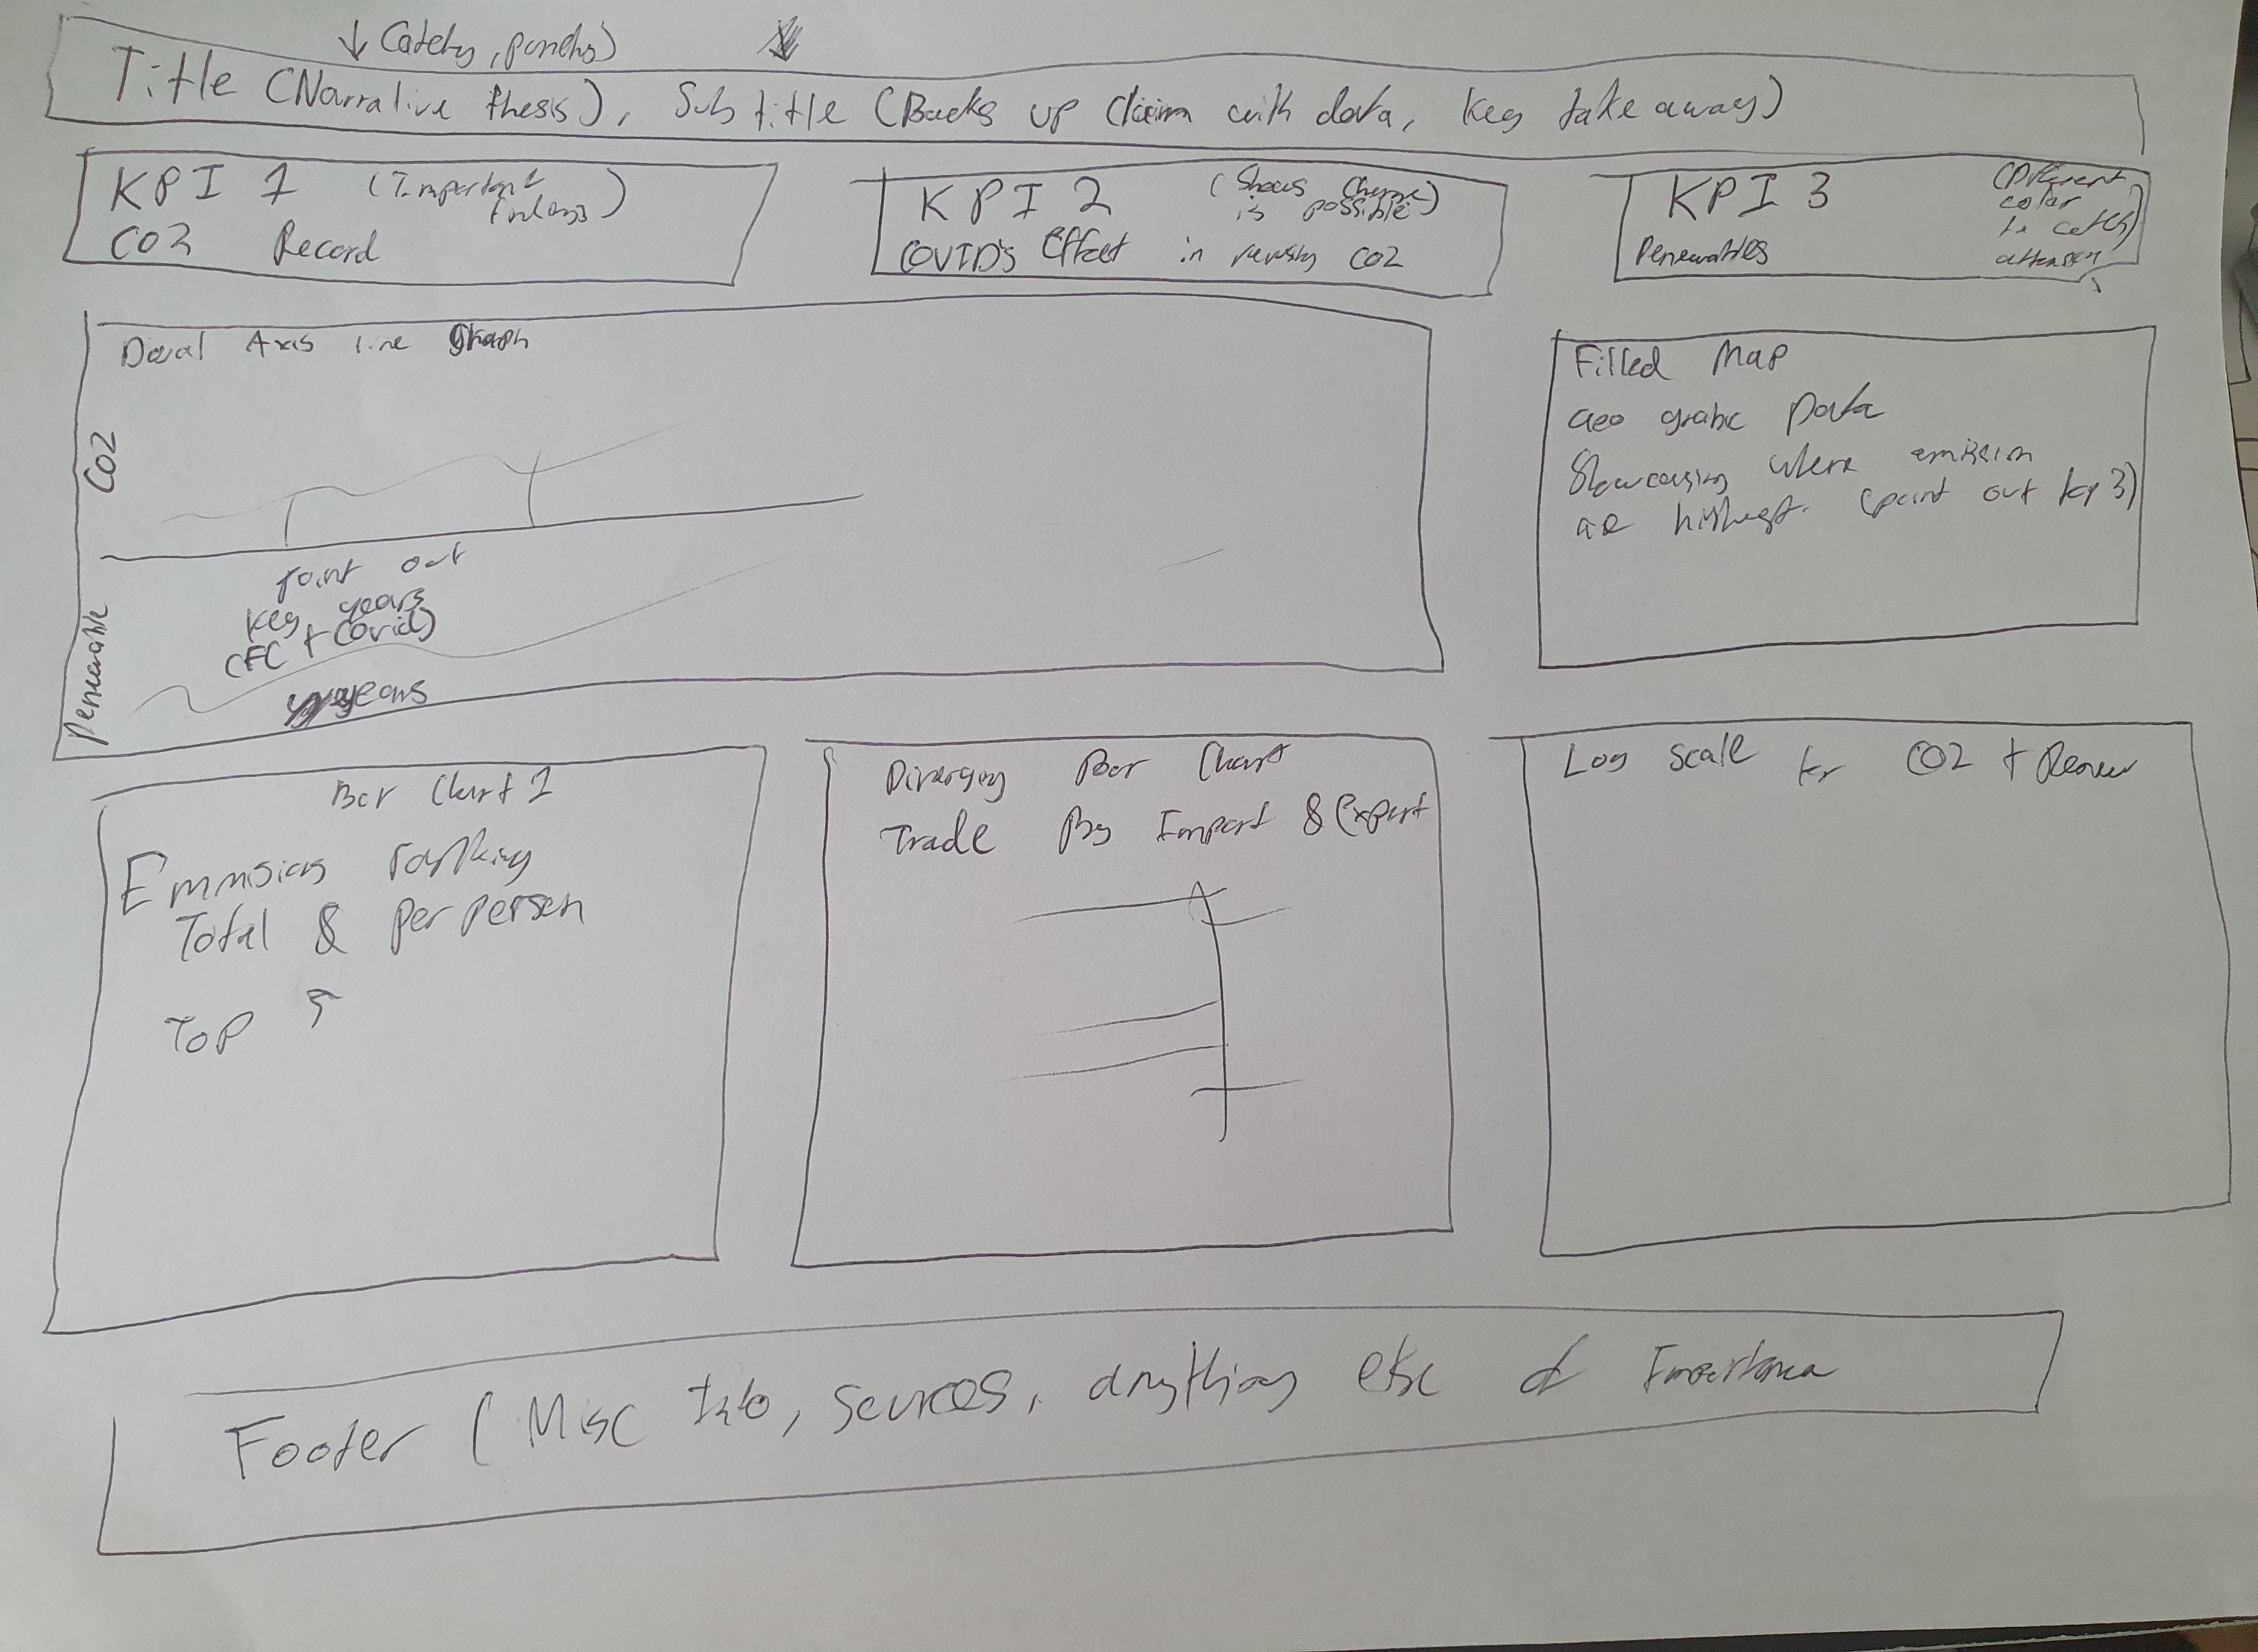
\includegraphics[width=1\linewidth]{dashboard_sketch}

\subsection{Dashboard Implementation (Self added
extension)}\label{dashboard-implementation-self-added-extension}

I wanted to extend my learning from this unit and build upon my Data
Science skills, so I challenged myself to create a proper Dashboard
using the data from this assessment built in Python, the code used is
included within the files.

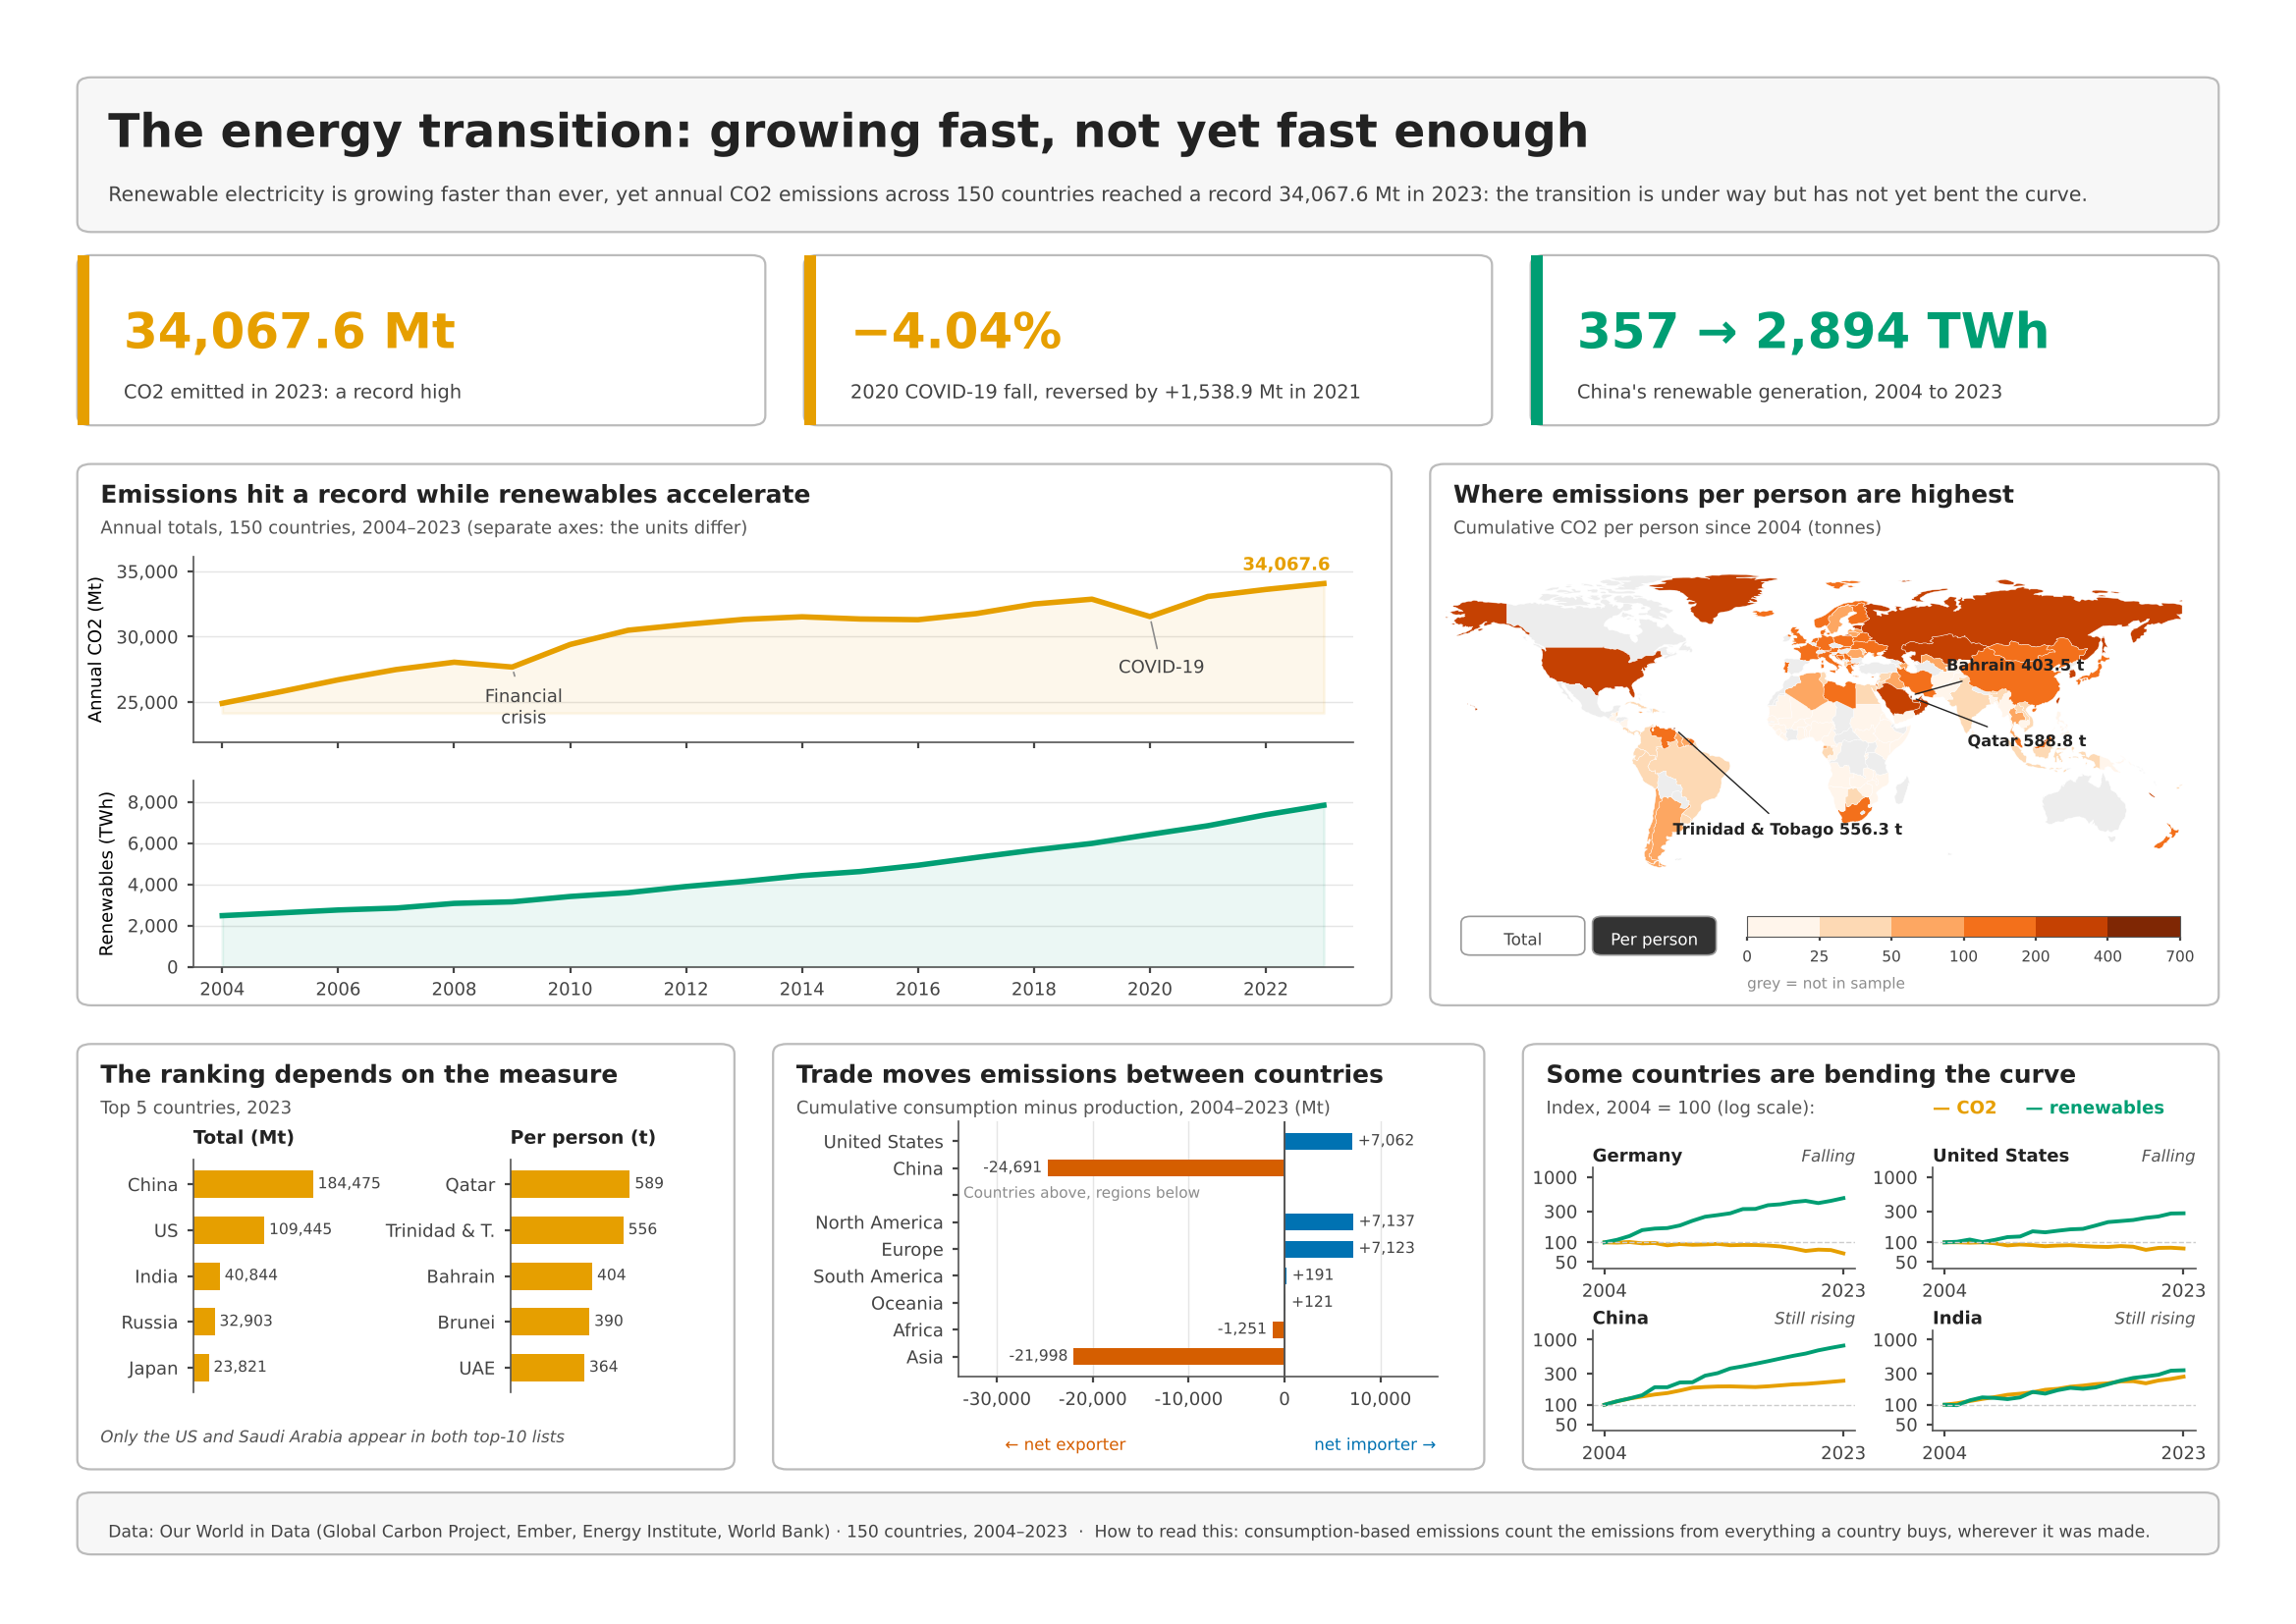
\includegraphics[width=1\linewidth]{dashboard_challenge}

\subsection{4.1 Data augmentation}\label{data-augmentation}

\emph{How would you augment this dataset for a comprehensive view of the
transition? What sources, and what would each add?}

The current dataset shows how much renewable electricity each country
generates, but not what share of its electricity this represents, and it
holds only one year of population and GDP. I would bring in five
additional sources to address these gaps. First, electricity generation
by source from Ember and the Our World in Data energy dataset would
convert renewable output in TWh into a renewable \emph{share} of total
generation, which is the measure that shows whether clean power is
displacing fossil power or simply meeting new demand. Second, primary
energy consumption by fuel from the Energy Institute Statistical Review
would separate coal, oil and gas, explaining why some countries'
emissions fall faster than others' (and providing the
\texttt{CumFossilEnergy} feature proposed in 3B). Third, annual
population estimates from the UN World Population Prospects and annual
GDP from the World Bank's World Development Indicators would replace the
static 2022 values, allowing per-capita emissions and the carbon
intensity of GDP to be tracked year by year. Fourth, the full Global
Carbon Project series, including land-use change and all countries,
would complete the global picture; Australia, for example, is absent
from my 150-country sample. Finally, national targets from the UNFCCC
and Climate Action Tracker would let the dashboard compare each
country's actual trajectory with its pledges, turning a description of
the past into an assessment of progress.

\subsection{4.2 Key insights}\label{key-insights}

The dashboard highlights five insights, each mapped to one panel. The
headline (KPI tiles and Panel 1) is that annual emissions reached a
record 34,067.6 Mt in 2023. The only notable falls were in 2009 (-371.8
Mt) and 2020 (-1,329.5 Mt, -4.04\%), and the 2020 fall reversed within a
year (+1,538.9 Mt in 2021), showing that temporary shocks do not change
the trend. Panel 1 pairs this with renewable generation on an aligned
time axis, because the contrast between an accelerating renewables curve
and a still-rising emissions line \emph{is} the thesis.

Panel 2, a choropleth map of cumulative emissions per person, gives
readers a geographic entry point and lets them locate their own region.
Panel 3 shows that responsibility depends on the measure: China leads
cumulative emissions (184,474.9 Mt), but Qatar leads per person (588.8
t, 4.5 times China's 129.4 t), and only the United States and Saudi
Arabia appear in both top 10 lists. Side-by-side bar charts are chosen
because ranked bars make this reversal immediate. Panel 4, a diverging
bar chart, shows that trade moves emissions between countries: the
United States consumed 7,062.2 Mt more than it produced, while China
produced 24,691.0 Mt more than it consumed. Panel 5 uses small multiples
to show diverging pathways: in Germany and the United States emissions
fall as renewables rise (Germany's renewables grew from 57.97 to 277.1
TWh), while in China and India emissions keep climbing despite rapid
renewable growth. Small multiples with shared scales let readers compare
shapes without reading exact values.

\textbf{YOUR ANSWER}

\subsection{4.3 Design elements}\label{design-elements}

\emph{Layout, colour, typography, placement.}

The layout follows the order in which a reader scans a page, top-left to
bottom-right. Three KPI tiles sit beneath the title so the core story is
visible in seconds, the largest panel (Panel 1) carries the thesis in
the upper left, and supporting panels follow in a row beneath. A
12-column grid with generous white space keeps the five panels distinct.
Colour is used consistently and sparingly: orange always means emissions
and bluish-green always means renewables, drawn from the
colourblind-safe Okabe--Ito palette so that the two never rely on a
red--green contrast. The map uses a single-hue sequential scale, and
neutral grey is reserved for context such as gridlines. Typography uses
one clean sans-serif typeface in a clear hierarchy: a large title, large
bold numbers for the KPIs, medium panel titles and small axis labels.
Every panel title states its takeaway in plain language (``Emissions hit
a record in 2023'') rather than naming its variables, and annotations
such as ``COVID-19'' are placed directly on the lines instead of in a
separate legend.

\subsection{4.4 Audience consideration}\label{audience-consideration}

\emph{How does the design serve a public audience --- accessible,
understandable, actionable?}

The design serves a public audience in three ways. It is
\emph{accessible}: the colourblind-safe palette, high-contrast text,
large fonts, direct labels and alternative text for each chart allow
readers with visual impairments or on small screens to follow it. It is
\emph{understandable}: each panel carries a single message, technical
terms are explained in a ``How to read this'' box (for example,
``consumption-based emissions count the emissions from everything a
country buys, wherever it was made''), and quantities are expressed in
relatable units such as tonnes per person. It is \emph{actionable}: the
per-capita map and the total-versus-per-person toggle let readers place
their own country in context, Panel 5 shows that falling emissions are
achievable alongside rising renewables, and the footer notes the data's
limits (the record begins in 2004 and covers 150 countries) so readers
do not over-interpret it.

\subsection{4.5 Additional questions}\label{additional-questions}

\emph{One relevant metric or visualisation you deliberately omitted, and
why omitting it serves clarity.}

I deliberately omitted the regression results from Task 3, including the
correlation of 0.98 between cumulative emissions and GDP and the model
RMSE values. They are relevant because they show how closely emissions
track economic size, but they require statistical literacy to read, and
my assumption checks showed that the linear model violates linearity,
normality and constant variance, so a public reader could take a
headline such as ``GDP explains 81\% of emissions'' as causal fact.
Leaving the models out keeps every panel focused on the thesis and
avoids presenting a fragile statistical result as a firm conclusion.

\emph{One way your dashboard could be misread, and how design mitigates
it.}

The choropleth map (Panel 2) could be misread because map area is
unrelated to emissions: physically large countries dominate the eye,
while the per-capita leaders (Qatar, Bahrain, and Trinidad and Tobago)
are tiny and almost invisible. A reader could wrongly conclude that the
largest countries have the highest per-person emissions. To mitigate
this, the map shows a per-capita rate rather than totals, so area is not
compounded by size; callout labels point to the small high-emitting
states; and Panel 3 places a ranked bar chart beside the map, where
every country gets a bar of equal visual weight.

\emph{Does your headline figure use total or per-capita emissions?
Defend that choice against the obvious objection.}

The headline uses total emissions: 34,067.6 Mt in 2023. The obvious
objection is that totals unfairly emphasise populous countries and hide
the fact that someone in Qatar is associated with 588.8 t of cumulative
CO2 against 28.7 t in India. I chose totals because the atmosphere
responds to total tonnes emitted, not to emissions per person, and the
thesis asks whether the global curve is bending. The headline is also a
sum across all countries, so it singles out no nation. The fairness
concern is addressed directly rather than hidden: Panel 3 sets
per-person rankings beside totals, Panel 4 adjusts for trade, and the
map shows per-capita emissions, so a reader can see both the scale of
the problem and how unevenly it is shared.

\newpage

\section{Conclusions}\label{conclusions}

\emph{What are the main things your analysis shows? Keep it grounded in
your own numbers.}

The central finding of this analysis is that the energy transition is
real but has not yet bent the emissions curve. Across my 150 countries,
annual production-based emissions reached a record 34,067.6 Mt in 2023.
The only meaningful falls in twenty years came from external shocks
rather than policy: the financial crisis in 2009 (-371.8 Mt) and the
COVID-19 pandemic in 2020 (-1,329.5 Mt, -4.04\%), the latter fully
reversed by a 1,538.9 Mt rebound in 2021. Renewable generation, by
contrast, accelerated throughout the period; China's alone rose
eightfold, from 357.43 to 2,894.22 TWh. Yet even the fastest renewable
growth in the dataset has so far added to fossil supply rather than
replaced it, while Germany, Japan and the United States show that
emissions can fall as renewables rise.

A second finding is that who appears responsible depends on how
emissions are measured. Emissions are highly concentrated: Asia accounts
for 57\% of the cumulative total and China alone for 30\% (184,474.9
Mt). Per person, however, the leader is Qatar at 588.8 t, 4.5 times
China's 129.4 t, and only the United States and Saudi Arabia appear in
both top 10 rankings. Trade shifts the picture again: the United States
consumed 7,062.2 Mt more than it produced, while China produced 24,691.0
Mt more than it consumed. No single measure is neutral, which matters
for any policy that allocates responsibility.

The modelling showed how easily a strong statistic can mislead. GDP
correlates 0.98 with cumulative emissions, but GDP per capita correlates
only 0.12, revealing that the relationship mostly reflects country size
rather than wealth. The full linear model's apparent accuracy (test RMSE
647.46 Mt against 1,719.84 Mt for GDP alone) came largely from
\texttt{CumConsCO2}, which is near-identical to the target, and every
regression diagnostic failed under the influence of China, India and the
United States. A log-log model (577.66 Mt) handled the skewed data
better, which was a lesson in matching the method to the data's
distribution.

The main challenge throughout was distinguishing errors from genuine
extremes. Some defects were obvious once tested against physical limits,
such as Sweden's negative 2022 emissions. Others were silent and would
have passed unnoticed without cross-checks: Chile's population was
recorded as 19,553, detectable only because GDP divided by GDP per
capita implied 19.55 million, and five oil values were the code -999.
Equally, genuine extremes had to be protected: the rapid renewable
growth of countries like the UAE would have been deleted by an automatic
spike rule, and China could not be removed simply because it distorted
the model. Each imputation choice also carried consequences; assigning
zero consumption to the 55 uncovered countries would have turned every
one of them into an extreme carbon exporter. The most important lesson I
take from this work is that data cleaning is not a mechanical step
before the analysis but a series of judgements that shape the results,
and that each of those judgements needs evidence, not intuition.

\newpage

\section{Section 5: Verification}\label{section-5-verification}

\subsection{5.1 Results Summary Table}\label{results-summary-table}

\begin{Shaded}
\begin{Highlighting}[]
\CommentTok{\# Prints every value needed for the table below, straight from the}
\CommentTok{\# objects computed above, so the table can be filled in without retyping}
\CommentTok{\# numbers by hand from different sections.}
\NormalTok{neg\_label }\OtherTok{\textless{}{-}} \ControlFlowTok{if}\NormalTok{ (}\FunctionTok{nrow}\NormalTok{(negative\_rows) }\SpecialCharTok{==} \DecValTok{0}\NormalTok{) }\StringTok{"none"} \ControlFlowTok{else}
  \FunctionTok{paste}\NormalTok{(}\FunctionTok{paste}\NormalTok{(negative\_rows}\SpecialCharTok{$}\NormalTok{Country, negative\_rows}\SpecialCharTok{$}\NormalTok{Year), }\AttributeTok{collapse =} \StringTok{"; "}\NormalTok{)}

\FunctionTok{cat}\NormalTok{(}\StringTok{" 1. Fingerprint:"}\NormalTok{, my}\SpecialCharTok{$}\NormalTok{fingerprint, }\StringTok{"}\SpecialCharTok{\textbackslash{}n}\StringTok{"}\NormalTok{,}
    \StringTok{"2. First and last year:"}\NormalTok{, }\FunctionTok{min}\NormalTok{(master}\SpecialCharTok{$}\NormalTok{Year), }\StringTok{"{-}"}\NormalTok{, }\FunctionTok{max}\NormalTok{(master}\SpecialCharTok{$}\NormalTok{Year),}
    \StringTok{"}\SpecialCharTok{\textbackslash{}n}\StringTok{"}\NormalTok{,}
    \StringTok{"3. Countries in Emissions.csv:"}\NormalTok{, n\_countries, }\StringTok{"}\SpecialCharTok{\textbackslash{}n}\StringTok{"}\NormalTok{,}
    \StringTok{"4. dim(master):"}\NormalTok{, }\FunctionTok{paste}\NormalTok{(}\FunctionTok{dim}\NormalTok{(master), }\AttributeTok{collapse =} \StringTok{" x "}\NormalTok{), }\StringTok{"}\SpecialCharTok{\textbackslash{}n}\StringTok{"}\NormalTok{,}
    \StringTok{"5. Duplicate rows removed:"}\NormalTok{, n\_dup\_removed, }\StringTok{"}\SpecialCharTok{\textbackslash{}n}\StringTok{"}\NormalTok{,}
    \StringTok{"6. Negative{-}emissions rows:"}\NormalTok{, neg\_label, }\StringTok{"}\SpecialCharTok{\textbackslash{}n}\StringTok{"}\NormalTok{,}
    \StringTok{"7. Countries with no consumption data:"}\NormalTok{, n\_no\_cons, }\StringTok{"}\SpecialCharTok{\textbackslash{}n}\StringTok{"}\NormalTok{,}
    \StringTok{"8. Highest{-}CO2 year and total:"}\NormalTok{, peak\_year}\SpecialCharTok{$}\NormalTok{Year, }\StringTok{"/"}\NormalTok{,}
    \FunctionTok{round}\NormalTok{(peak\_year}\SpecialCharTok{$}\NormalTok{TotalCO2, }\DecValTok{1}\NormalTok{), }\StringTok{"Mt}\SpecialCharTok{\textbackslash{}n}\StringTok{"}\NormalTok{,}
    \StringTok{"9. Top cumulative / per capita:"}\NormalTok{, top10total}\SpecialCharTok{$}\NormalTok{Country[}\DecValTok{1}\NormalTok{], }\StringTok{"/"}\NormalTok{,}
\NormalTok{    top10percap}\SpecialCharTok{$}\NormalTok{Country[}\DecValTok{1}\NormalTok{], }\StringTok{"}\SpecialCharTok{\textbackslash{}n}\StringTok{"}\NormalTok{,}
    \StringTok{"10. cor(CumCO2, GDP) / cor(CumCO2, GDPCapita):"}\NormalTok{, }\FunctionTok{round}\NormalTok{(cor\_gdp, }\DecValTok{2}\NormalTok{),}
    \StringTok{"/"}\NormalTok{, }\FunctionTok{round}\NormalTok{(cor\_gdp\_pc, }\DecValTok{2}\NormalTok{), }\StringTok{"}\SpecialCharTok{\textbackslash{}n}\StringTok{"}\NormalTok{,}
    \StringTok{"11. Test RMSE, GDP{-}only model:"}\NormalTok{, }\FunctionTok{round}\NormalTok{(rmse\_gdp, }\DecValTok{2}\NormalTok{), }\StringTok{"}\SpecialCharTok{\textbackslash{}n}\StringTok{"}\NormalTok{,}
    \StringTok{"12. Test RMSE, full model:"}\NormalTok{, }\FunctionTok{round}\NormalTok{(rmse\_full, }\DecValTok{2}\NormalTok{), }\StringTok{"}\SpecialCharTok{\textbackslash{}n}\StringTok{"}\NormalTok{,}
    \StringTok{"13. High{-}leverage country:"}\NormalTok{, high\_lev\_country, }\StringTok{"}\SpecialCharTok{\textbackslash{}n}\StringTok{"}\NormalTok{)}
\end{Highlighting}
\end{Shaded}

\begin{verbatim}
##  1. Fingerprint: EM-606669-0798-6584 
##  2. First and last year: 2004 - 2023 
##  3. Countries in Emissions.csv: 150 
##  4. dim(master): 3000 x 26 
##  5. Duplicate rows removed: 5 
##  6. Negative-emissions rows: Equatorial Guinea 2010; Sri Lanka 2012; Sudan 2018; Sweden 2022 
##  7. Countries with no consumption data: 55 
##  8. Highest-CO2 year and total: 2023 / 34067.6 Mt
##  9. Top cumulative / per capita: China / Qatar 
##  10. cor(CumCO2, GDP) / cor(CumCO2, GDPCapita): 0.98 / 0.12 
##  11. Test RMSE, GDP-only model: 1719.84 
##  12. Test RMSE, full model: 647.46 
##  13. High-leverage country: China
\end{verbatim}

\emph{Fill every cell by hand from your own output. If you could not
compute one, write \texttt{NA} and say why in a footnote below the
table.}

{\def\LTcaptype{none} % do not increment counter
\begin{longtable}[]{@{}
  >{\raggedright\arraybackslash}p{(\linewidth - 4\tabcolsep) * \real{0.3333}}
  >{\raggedright\arraybackslash}p{(\linewidth - 4\tabcolsep) * \real{0.3333}}
  >{\raggedright\arraybackslash}p{(\linewidth - 4\tabcolsep) * \real{0.3333}}@{}}
\toprule\noalign{}
\begin{minipage}[b]{\linewidth}\raggedright
\#
\end{minipage} & \begin{minipage}[b]{\linewidth}\raggedright
Quantity
\end{minipage} & \begin{minipage}[b]{\linewidth}\raggedright
Your value
\end{minipage} \\
\midrule\noalign{}
\endhead
\bottomrule\noalign{}
\endlastfoot
1 & Dataset fingerprint (printed by the setup chunk) &
EM-606669-0798-6584 \\
2 & First and last year in your dataset & 2004 and 2023 \\
3 & Number of countries in your \texttt{Emissions.csv} & 150 \\
4 & \texttt{dim()} of your final merged master data frame & 3000 x 26 \\
5 & Number of duplicate rows you removed in Task 1 & 5 \\
6 & Countries and years of the negative-emissions rows (1A ii) &
Equatorial Guinea 2010; Sri Lanka 2012; Sudan 2018; Sweden 2022 \\
7 & Number of countries with no consumption-based data (1A iii) & 55 \\
8 & Year with the highest total CO2, and that total (Task 2.1) & 2023,
34,067.6 Mt \\
9 & Top country by cumulative emissions, and by emissions per capita &
China (cumulative); Qatar (per capita) \\
10 & \texttt{cor(CumCO2,\ GDP)} and \texttt{cor(CumCO2,\ GDPCapita)} (2
dp) & 0.98 and 0.12 \\
11 & Test RMSE of the GDP-only model (Task 3.5) & 1,719.84 Mt \\
12 & Test RMSE of the full model (Task 3.6) & 647.46 Mt \\
13 & The high-leverage country you identified (3A iv) & China \\
\end{longtable}
}

\subsection{5.2 Reproducibility
appendix}\label{reproducibility-appendix}

\emph{Run this chunk unchanged. Do not edit it.}

\begin{Shaded}
\begin{Highlighting}[]
\FunctionTok{cat}\NormalTok{(}\StringTok{"Student ID  :"}\NormalTok{, params}\SpecialCharTok{$}\NormalTok{studentID, }\StringTok{"}\SpecialCharTok{\textbackslash{}n}\StringTok{"}\NormalTok{)}
\end{Highlighting}
\end{Shaded}

\begin{verbatim}
## Student ID  : u3284342
\end{verbatim}

\begin{Shaded}
\begin{Highlighting}[]
\FunctionTok{cat}\NormalTok{(}\StringTok{"Fingerprint :"}\NormalTok{, my}\SpecialCharTok{$}\NormalTok{fingerprint, }\StringTok{"}\SpecialCharTok{\textbackslash{}n}\StringTok{"}\NormalTok{)}
\end{Highlighting}
\end{Shaded}

\begin{verbatim}
## Fingerprint : EM-606669-0798-6584
\end{verbatim}

\begin{Shaded}
\begin{Highlighting}[]
\FunctionTok{cat}\NormalTok{(}\StringTok{"Window      :"}\NormalTok{, }\FunctionTok{paste}\NormalTok{(my}\SpecialCharTok{$}\NormalTok{window, }\AttributeTok{collapse =} \StringTok{" {-} "}\NormalTok{), }\StringTok{"}\SpecialCharTok{\textbackslash{}n}\StringTok{"}\NormalTok{)}
\end{Highlighting}
\end{Shaded}

\begin{verbatim}
## Window      : 2004 - 2023
\end{verbatim}

\begin{Shaded}
\begin{Highlighting}[]
\FunctionTok{cat}\NormalTok{(}\StringTok{"Knitted at  :"}\NormalTok{, }\FunctionTok{format}\NormalTok{(}\FunctionTok{Sys.time}\NormalTok{(), }\StringTok{"\%Y{-}\%m{-}\%d \%H:\%M:\%S \%Z"}\NormalTok{), }\StringTok{"}\SpecialCharTok{\textbackslash{}n}\StringTok{"}\NormalTok{)}
\end{Highlighting}
\end{Shaded}

\begin{verbatim}
## Knitted at  : 2026-11-10 21:49:05 AEDT
\end{verbatim}

\begin{Shaded}
\begin{Highlighting}[]
\FunctionTok{cat}\NormalTok{(}\StringTok{"Chunks run  :"}\NormalTok{, }\FunctionTok{length}\NormalTok{(knitr}\SpecialCharTok{::}\FunctionTok{all\_labels}\NormalTok{()), }\StringTok{"}\SpecialCharTok{\textbackslash{}n\textbackslash{}n}\StringTok{"}\NormalTok{)}
\end{Highlighting}
\end{Shaded}

\begin{verbatim}
## Chunks run  : 45
\end{verbatim}

\begin{Shaded}
\begin{Highlighting}[]
\FunctionTok{print}\NormalTok{(}\FunctionTok{sessionInfo}\NormalTok{()}\SpecialCharTok{$}\NormalTok{R.version}\SpecialCharTok{$}\NormalTok{version.string)}
\end{Highlighting}
\end{Shaded}

\begin{verbatim}
## [1] "R version 4.6.1 (2026-06-24)"
\end{verbatim}

\newpage

\section{Appendix: Decision Log}\label{appendix-decision-log}

\emph{Minimum five entries. Write each one \textbf{at the time you make
the decision}, not at the end. Every entry must reference something
specific from your own analysis --- a variable name, a country, a line
of code, an output value. Generic entries receive zero marks. Add rows
freely; more than five is viewed favourably.}

{\def\LTcaptype{none} % do not increment counter
\begin{longtable}[]{@{}
  >{\raggedright\arraybackslash}p{(\linewidth - 10\tabcolsep) * \real{0.1667}}
  >{\raggedright\arraybackslash}p{(\linewidth - 10\tabcolsep) * \real{0.1667}}
  >{\raggedright\arraybackslash}p{(\linewidth - 10\tabcolsep) * \real{0.1667}}
  >{\raggedright\arraybackslash}p{(\linewidth - 10\tabcolsep) * \real{0.1667}}
  >{\raggedright\arraybackslash}p{(\linewidth - 10\tabcolsep) * \real{0.1667}}
  >{\raggedright\arraybackslash}p{(\linewidth - 10\tabcolsep) * \real{0.1667}}@{}}
\toprule\noalign{}
\begin{minipage}[b]{\linewidth}\raggedright
\#
\end{minipage} & \begin{minipage}[b]{\linewidth}\raggedright
Task \& step
\end{minipage} & \begin{minipage}[b]{\linewidth}\raggedright
Decision made
\end{minipage} & \begin{minipage}[b]{\linewidth}\raggedright
Alternative considered
\end{minipage} & \begin{minipage}[b]{\linewidth}\raggedright
Why I chose this
\end{minipage} & \begin{minipage}[b]{\linewidth}\raggedright
Impact on results
\end{minipage} \\
\midrule\noalign{}
\endhead
\bottomrule\noalign{}
\endlastfoot
1 & 1.1 Import (\texttt{ReadRaw()}) & Read every column as text
(\texttt{col\_types\ =\ cols(.default\ =\ col\_character())},
\texttt{trim\_ws\ =\ FALSE}) & Let \texttt{read\_csv()} guess column
types & Type guessing would silently coerce comma-formatted numbers and
strip padded ISO codes, hiding the defects before they could be counted
& 5 comma-formatted \texttt{Consumption\ CO2} values (e.g.~China 2018,
``9,443.433'') and 76 padded ISO codes were detected and logged instead
of lost \\
2 & 1.2 Renewables join key (\texttt{NormaliseName()},
\texttt{name\_fixes}) & Mapped \texttt{Country.Region} names to ISO
codes via normalised names and a spelling-variant list & Join on the raw
country name & Renewables.csv has no ISO column, and names such as
``Egypt, Arab Rep.'' and ``Burma'' do not match Emissions.csv exactly &
All 6 variant names matched; the 1.5 join report shows 0 unused
renewables rows \\
3 & 1.2 Non-country rows (\texttt{renew\_non\_country}) & Removed
``World'' and ``European Union (27)'' & Keep them in a separate data
frame as a check on totals & Both are sums of countries already present
(e.g.~France, Germany), so they would double-count renewables in Task 2
& 40 country-year rows removed; Renewables matched to 146 countries \\
4 & 1.4 Year type (\texttt{ParseYear()}) & Stored \texttt{Year} as a
four-digit integer in every data frame & Convert to \texttt{Date} (1
January of each year) & All data are annual; an integer joins exactly
and supports \texttt{Year\ \%/\%\ 10} and
\texttt{Year\ \textless{}\ 2016} without inventing a day and month & 114
Consumption values in three formats (``FY2004'', ``01/01/2009'',
``2010.0'') converted with 0 failures; 0 Consumption rows unused in the
join \\
5 & 1.4b Negative CO2 (\texttt{negative\_rows}) & Set the 4 negative
\texttt{CO2} values to NA and interpolated from neighbouring years &
Take the absolute value & The neighbours show the magnitude is also
wrong: Sweden emitted 38.568 Mt in 2021 and 36.709 Mt in 2023, so
flipping -2.594 would still be about 93\% too low & Sweden 2022 became
37.64 Mt; Equatorial Guinea 2010 5.47, Sri Lanka 2012 14.31, Sudan 2018
21.16 \\
6 & 1.4b Missing-value codes in OilCO2 (\texttt{sentinel\_values}) &
Treated -999 as missing and interpolated & Treat it as a negative value,
or set it to 0 & -999 is a placeholder, not a measurement; left in, it
would subtract 999 Mt from \texttt{CumOilCO2} & 5 rows repaired
(e.g.~Qatar 2016, Zimbabwe 2010); OilCO2 had 0 NAs after 1.6 \\
7 & 1.4b GDP consistency (\texttt{ctry\_inconsistent}) & Replaced
Chile's \texttt{Population} (19,553) with the population implied by GDP
and GDPCapita & Recompute Chile's \texttt{GDPCapita} from GDP and
Population & GDP (448,338) and GDPCapita (22,929) agree with each other,
so Population is the inconsistent value (ratio 0.001) & Chile's
population became 19,553,317; otherwise its per-capita values would have
been about 1,000 times too large \\
8 & 1.6 Consumption coverage (\texttt{ConsImputed}) & Set
\texttt{ConsCO2\ =\ CO2} for the 55 countries with no consumption data &
Replace with 0 & Zero gives \texttt{NetImported\ =\ -CumCO2}, a share of
-1, far outside the observed range among covered countries (-0.49 to
2.572) & Algeria's NetImported is 0 instead of -2,898.4 Mt; the 55
countries are flagged and excluded from the 3B evidence \\
9 & 3.8 Extension model (\texttt{model\_log}) & Added a log-log linear
model to the comparison & Use only the suggested ridge, lasso and tree &
3.3 and the Shapiro test (W = 0.236 raw vs 0.994 logged) showed
\texttt{CumCO2} is heavily right-skewed & Best test RMSE of all models:
577.66 Mt (R² 0.979) vs 647.46 Mt for the full linear model \\
10 & 3A iv Influential observation (\texttt{high\_lev\_country}) &
Identified China as the high-leverage point but kept it in the reported
models & Drop China permanently because it improves RMSE & China's
values are genuine and it is the largest emitter; dropping it hides the
most policy-relevant country & Test RMSE would fall from 647.46 to
546.71 Mt without China, but the log model (577.66 Mt) improves fit
while keeping it \\
\end{longtable}
}

\begin{center}\rule{0.5\linewidth}{0.5pt}\end{center}

\section{Declaration}\label{declaration}

\begin{quote}
I confirm that the dataset analysed in this submission was generated
from my own student ID, that the values reported in Section 5.1 are the
values produced by the code in this document, and that all explanations
and interpretations are my own work.

\textbf{Student ID:} u3284342 \textbf{Date:} 10/11/26
\end{quote}

\end{document}
